%%%%%%%%%%%%%%%%%%%%%%%%%%%%%%%%%%%%%%%%%%%%%%%%%%%%%%%%%%%%%%%%%%%%%%%%%%%%%%
% ASU Dissertation Template
%%%%%%%%%%%%%%%%%%%%%%%%%%%%%%%%%%%%%%%%%%%%%%%%%%%%%%%%%%%%%%%%%%%%%%%%%%%%%%
% Copyright 2020 Robert W. Kutter (robert@kutterconsulting.com)
%
%   See also: http://kutterconsulting.com
%
% For guidance on using this file, see the README.
%
%%%%%%%%%%%%%%%%%%%%%%%%%%%%%%%%%%%%%%%%%%%%%%%%%%%%%%%%%%%%%%%%%%%%%%%%%%%%%%
% Preamble
%%%%%%%%%%%%%%%%%%%%%%%%%%%%%%%%%%%%%%%%%%%%%%%%%%%%%%%%%%%%%%%%%%%%%%%%%%%%%%
\newcommand*{\pointsize}{12pt}          %<Set the font size; make sure the size is correct
                                        %   for the font you will use
\documentclass[letterpaper,             % Use US letter-size paper
               oneside,                 % No verso and recto differences
               \pointsize]              % Uses the font size defined above
               {memoir}
\renewcommand{\cleardoublepage}%        % \cleardoublepage will create entirely blank
  {\clearpage}%                         %   pages depending on settings (e.g., usually
                                        %   before start of \mainmatter); redefine it here
                                        %   so that no entirely blank pages are created
                                        %   automatically
%%%%%%%%%%%%%%%%%%%%%%%%%%%%%%%%%%%%%%%
% (Some) Packages
%%%%%%%%%%%%%%%%%%%%%%%%%%%%%%%%%%%%%%%
\usepackage{csvsimple} 
\usepackage{booktabs}
\usepackage[section]{placeins}
\usepackage{graphicx}                   % For importing image files
% \usepackage{pgfplotstable} 
% \usepackage{longtable}
\usepackage{etoolbox}                   % For advanced commands throughout preamble
\usepackage{microtype}                  %~Improves kerning and protrusion (optional);
                                        %   See here for an introduction:
                                        %   http://www.khirevich.com/latex/microtype/
\usepackage{listings}                                        
\lstset{
basicstyle=\small\ttfamily,
columns=flexible,
breaklines=true
}
\providetoggle{usemicrotype}            % TRUE = microtype is being used
\makeatletter                           %   (Used to turn of microtype protrusion in the
\@ifpackageloaded{microtype}%           %   table of contents.)
  {\settoggle{usemicrotype}{true}}%
  {\settoggle{usemicrotype}{false}}
\makeatother
\usepackage{changepage}                 % For changing page layout (e.g., margins) in the
                                        %   middle of the document
\usepackage{calc}					              % Calculate text widths; used in page layout
                                        %   changes

%%%%%%%%%%%%%%%%%%%%%%%%%%%%%%%%%%%%%%%
% Title page, input
%%%%%%%%%%%%%%%%%%%%%%%%%%%%%%%%%%%%%%%
\listadd{\titlelines}%
  {Augmenting Academic Research Search And Reading With}             %<Enter the title of the dissertation
\listadd{\titlelines}%
  {Richer Context}            % If you want to
                                        %   split the title across lines,
                                        %   use another \listadd command for the
                                        %   second line
\newcommand*\Author{Valay Gaurang Dave}          %<Enter your name; must match official transcript
\newcommand*{\documentname}%
  {Dissertation}                        %<Enter the type of document (capitalized)
\newcommand*{\degreename}
  {Master Of Science}                %<Enter the type of degree (capitalized)
\newcommand*\defdate{April 2021}        %<Give month (written out fully) and year of
                                        %   the oral defense
\listadd{\committeechair}{Jia Zou}   %<Enter committee chair name; use \listadd for
\listadd{\committeechair}{Heni Ben Amor}%   for additional names
\newcommand*{\chairlabel}{Co-Chair}        %<If you have co-chairs, replace this text with
                                        %   'Co-Chair'
\listadd{\committeemember}{Kasim Selcuk Candan} %<Enter committee member names; use \listadd for
% \newcommand*{\committeelabel}{Member}
\newcommand*{\gradmonth}{May}           %<Enter the graduation date; month can only be:
                                        %  May, August, or December
\newcommand*{\gradyear}{2021}           %<Enter the graduation year, e.g. 2014

\listadd{\keywords}{academic research}          %<Enter keywords; use \listadd for
\listadd{\keywords}{search engine}          %   additional names (up to 6)
\listadd{\keywords}{table classification}
\newcommand*{\graddate}{\gradmonth%     % Compose full graduation date
  \space\gradyear}

%%%%%%%%%%%%%%%%%%%%%%%%%%%%%%%%%%%%%%%
% Page layout
%%%%%%%%%%%%%%%%%%%%%%%%%%%%%%%%%%%%%%%
\settrimmedsize{\stockheight}%          % Specifies \paperheight and \paperwidth
  {\stockwidth}{*}
\settrims{0pt}{0pt}                     % Set location of page in relation to the stock.
                                        % Paper and stock size are equivalent,
                                        % so both \trimtop and \trimedge are set to 0pt
\newlength{\forfootskip}
\setlength{\forfootskip}%
  {3\baselineskip}
\newlength{\textblockheight}            % Calculate height of text block to leave room
\setlength{\textblockheight}{9.0in}     %   for footers, keeping page numbers outside
\addtolength{\textblockheight}%         %   the 1in vertical margins
  {-\forfootskip}
\settypeblocksize{\textblockheight}%    % Calculated by 1.0in vertical margins and
  {*}{*}                                %   letting margins set the width of the typeblock
\setulmargins{1.0in}{*}{*}              % Set upper margin (\uppermargin, not \topmargin);
                                        %   calculate the bottom margin
\setlrmarginsandblock{1.25in}{1.25in}{*}%~Set margins and calculate width of typeblock
\setheaderspaces{*}{0.5\baselineskip}{*}% Arguments: '\headdrop', '\headsep', and/or ratio
                                        %   Note: This is only used in the list of
                                        %   contents sections
\setheadfoot{\baselineskip}%            % Set '\headheight' and '\footskip'
  {\forfootskip}
\checkandfixthelayout                   % Required by memoir package after setting layout
\settypeoutlayoutunit{in}               % Write layout dimensions to log file in inches

%%%%%%%%%%%%%%%%%%%%%%%%%%%%%%%%%%%%%%%
% Fonts
%%%%%%%%%%%%%%%%%%%%%%%%%%%%%%%%%%%%%%%
\usepackage[T1]{fontenc}                % Standard option to handle, e.g., accented
                                        %   characters like 'ö' better
\usepackage{amssymb,mathtools}          % For AMS-LaTeX, see here for more:
                                        %     http://www.ams.org/publications/authors/tex/amslatex
                                        % ('mathtools' loads and extends 'amsmath')
\usepackage{ifxetex,ifluatex}           % Can check if XeTeX or LuaTeX was used to typeset
\usepackage{fixltx2e}                   % Provides \textsubscript
\IfFileExists{upquote.sty}%             % Use upquote if available, for
  {\usepackage{upquote}}{}              %   straight quotes in verbatim environments

% Load fonts depending on the
%   typesetting engine
\ifnum 0\ifxetex 1\fi\ifluatex 1\fi=0   % If pdftex
  \usepackage[utf8]{inputenc}           %   'utf8' should match the encoding of this file
                                        %
                                        %~Set up your font in pdftex here
                                        %
\else 									                % If xetex or luatex
  \ifxetex                              % If xetex
    \usepackage{mathspec}               % Matches non-math open-type font to math
                                        %   open-type font (use 'mathspec' if you want to
                                        %   write math in unicode)
    \usepackage{xunicode}               % Convert LaTeX character macros to unicode
  \else                                 % If luatex\usepackage{fontspec}
    \usepackage{fontspec}               % Use fontspec for (open type) font selection
  \fi
  \defaultfontfeatures{Mapping=tex-text,% Font spec setting
    Scale=MatchLowercase}
  \newcommand*{\euro}{€}

  % Using fonts in XeLaTeX can be complicated; the following settings
  % work when this file is compiled inside the Docker container produced
  % by the `build.sh` script.
  %
  % Sometimes something simple like the following will work:
  %
  %   \setmainfont{Garamond}
  %
  % But often the easiest solution is to move font files (*.otf or *.ttf) into
  % a sub-directory and provide the direct path to them here.
  %
  % See `fontspec` documentation for more on using local font files.
  %
  \setmainfont{EBGaramond12}[           %<Set the main font; make sure the font is correct
                                        %   for the font size (See ASU Style Guide)
    Path          = /usr/share/fonts/opentype/ebgaramond/,
    Extension     = .otf ,
    UprightFont   = *-Regular ,
    ItalicFont    = *-Italic ,
    % Notice that bold is missing here because the Docker image does not have
    % a bold typeface for Garamond; it would probably be possible to find
    % one on your local system or online.
  ]

%  \setmathfont(Digits,Latin,Greek)%     %~Uncomment two lines to set a font for math%
%    {MATHFONT}
\fi

%%%%%%%%%%%%%%%%%%%%%%%%%%%%%%%%%%%%%%%
% Line spacing
%%%%%%%%%%%%%%%%%%%%%%%%%%%%%%%%%%%%%%%
\DoubleSpacing                          % True double spacing
\BeforeBeginEnvironment{quote}          % Memoir leaves most special material
  {\par\SingleSpacing}                  %   single spaced, but makes block quotes
\AfterEndEnvironment{quote}%            %   double-spaced; fix to follow ASU style guide
  {\vspace{-\baselineskip} %
  \DoubleSpacing}
\BeforeBeginEnvironment{quotation}%
  {\par\SingleSpacing}
\AfterEndEnvironment{quotation}%
  {\vspace{-\baselineskip} %
  \DoubleSpacing}

\setlength{\footnotesep}{\baselineskip} % Double space *between* footnotes
\renewcommand*{\footnoterule}{%         % Redefine footnoterule so that initial footnote
  \kern-3pt%                            %   still appears right under the rule (changing
  \hrule width 0.4\columnwidth          %   \footnotesep also changes the space between the
  \kern 2.6pt                           %   rule and the first footnote
  \vspace{-0.5\baselineskip}            % (Here is the vertical space adjustment)
  }

\usepackage{enumitem}                   % Control spacing in enumerate environment
\setlist{noitemsep}                     % Remove extra vertical spacing between items in lists
                                        % \setlist{nosep} to leave no space around whole list

%%%%%%%%%%%%%%%%%%%%%%%%%%%%%%%%%%%%%%%
% Page numbering
%%%%%%%%%%%%%%%%%%%%%%%%%%%%%%%%%%%%%%%
\makepagestyle{ASU}
  \makeevenfoot{ASU}{}{\thepage}{}
  \makeoddfoot{ASU}{}{\thepage}{}

%%%%%%%%%%%%%%%%%%%%%%%%%%%%%%%%%%%%%%%
% Title page, formatting
%%%%%%%%%%%%%%%%%%%%%%%%%%%%%%%%%%%%%%%
\newlength{\savedfootskip}
\setlength{\savedfootskip}{\footskip}
\newcommand{\titlepagesetup}{%          % Page layout for title page
  \changepage%                          % Adjustment to page dimensions:
    {\savedfootskip}%                   %   text height
    {}%                                 %   text width
    {}%                                 %   even-side margin
    {}%                                 %   odd-side margin
    {}%                                 %   column sep.
    {}%                                 %   topmargin
    {}%                                 %   headheight
    {}%                                 %   headsep
    {-\savedfootskip}%                  %   footskip
}

\newcommand{\closetitlepagesetup}{%     % Undo set up for title page
  \changepage{-\savedfootskip}{}{}{}{}%
    {}{}{}{\savedfootskip}%
}

\makeatletter                           % Do not modify this section; Enter info above
\newcommand*{\titlepageASU}{
  \titlepagesetup
  \clearpage
  \begin{center}
  \SingleSpacing
  \thispagestyle{empty}
    \renewcommand*{\do}[1]{##1 \\[\baselineskip]}
    \dolistloop{\titlelines}
    by \\[\baselineskip]
    \Author \\[5\baselineskip]
    A \documentname~Presented in Partial Fulfillment \\
    of the Requirements for the Degree \\
    \degreename \\
    \vfill                              % Vertically center the portion below
    Approved \defdate~by the \\
    Graduate Supervisory Committee: \\[\baselineskip]
    \renewcommand*{\do}[1]{##1, \chairlabel \\}
    \dolistloop{\committeechair}
    \renewcommand*{\do}[1]{##1 \\}
    \dolistloop{\committeemember}
    \vfill                              % Vertically center the portion above
    ARIZONA STATE UNIVERSITY \\[\baselineskip]
    \graddate
  \end{center}
  \clearpage
  \closetitlepagesetup
}
\makeatother

%%%%%%%%%%%%%%%%%%%%%%%%%%%%%%%%%%%%%%%
% Heading styles
%%%%%%%%%%%%%%%%%%%%%%%%%%%%%%%%%%%%%%%
% Note: memoir also has \book and \part commands; do not use these
\makechapterstyle{ASU}{%                % Define chapter heading style
  \renewcommand*{\chapterheadstart}{}   % Chapter title flush with top margin
  \renewcommand*{\chapnamefont}%        % Set font for 'Chapter' or 'Appendix'
    {\normalfont}
  \renewcommand*{\chapnumfont}%         % Set font for number in chapter headings
    {\normalfont}
  \renewcommand*{\afterchapternum}%     % Insert a double line break after
    {\\[\baselineskip]}                 %   chapter number
  \renewcommand*{\chaptitlefont}%       % Set font for chapter title name
    {\normalfont}
  \setlength{\afterchapskip}{0pt}       % Set vertical space between chapter title and
                                        %   first paragraph; equivalent to one line break
                                        %   (vertical space = \afterchapskip + \baselineskip)
                                        % Note: This \afterchapskip value is only used in
                                        %   front matter
  \renewcommand*{\printchapternum}{%    % Center justify chapter number
    \centering \chapnumfont %
    \thechapter}
  \renewcommand*{\printchaptertitle}[1]%% Center justify
    {\expandafter\centering %           %   \MakeUppercase has issues; see here for some
    \expandafter\chaptitlefont %        %   details: https://tex.stackexchange.com/questions/35680/uppercase-in-newcommand
    \expandafter\MakeUppercase %        %   Accented characters and some fonts may not
    \expandafter{##1}}                  %   uppercase correctly; if that happens, just
                                        %   type the chapter title in uppercase
}

\setsecnumdepth{all}                    %~Enter the levels that you want to have numbered
                                        %   (Default is to number all [5 levels deep].)

\newcommand{\divisionbeforeskip}%       % Create default formatting for headings
  {\baselineskip}
\newcommand{\divisionindent}%
  {0.5em}
\newcommand{\divisionfont}{\normalfont} % Font must be \normalfont
\newcommand{\divisionafterskip}%
  {\baselineskip}

\setbeforesecskip{\divisionbeforeskip}  % Apply default formatting to all heading levels
\setsecindent{\divisionindent}          % Note: If you change \setsecnumdepth above, you
\setsecheadstyle{\divisionfont}         %   will need to set the indent for all lower
\setaftersecskip{\divisionafterskip}    %   levels to '0pt'; otherwise, they will be
                                        %   preceded by unnecessary space
\setbeforesubsecskip{\divisionbeforeskip}
\setsubsecindent{\divisionindent}
\setsubsecheadstyle{\divisionfont}
\setaftersubsecskip{\divisionafterskip}

\setbeforesubsubsecskip{\divisionbeforeskip}
\setsubsubsecindent{\divisionindent}
\setsubsubsecheadstyle{\divisionfont}
\setaftersubsubsecskip{\divisionafterskip}

\setbeforeparaskip{\divisionbeforeskip}
\setparaindent{\divisionindent}
\setparaheadstyle{\divisionfont}
\setafterparaskip{\divisionafterskip}

\setbeforesubparaskip{\divisionbeforeskip}
\setsubparaindent{\divisionindent}
\setsubparaheadstyle{\divisionfont}
\setaftersubparaskip{\divisionafterskip}

%%%%%%%%%%%%%%%%%%%%%%%%%%%%%%%%%%%%%%%
% Paragraph formatting
%%%%%%%%%%%%%%%%%%%%%%%%%%%%%%%%%%%%%%%
%\sloppybottom                          % Reduce the chances of widows
\raggedbottom                           % Loosens vertical spacing requirements, so
                                        %   \sloppybottom doesn't make pages look bad;
                                        %   it also prevents large gaps in the middle of
                                        %   pages and pushes them to the bottom of pages
\indentafterchapter                     % Overrides the default which is not to indent
                                        %   the first paragraph in a chapter, but it
                                        %   looks odd in some places to not indent
                                        %   paragraphs

%%% List Titles %%%
\renewcommand{\contentsname}%           % Set heading for each list
  {Table of Contents}%                  %   Formatted as chapter headings by default, so
\renewcommand{\listtablename}%          %   no additional heading formatting is needed
  {List of Tables}
\renewcommand{\listfigurename}%
  {List of Figures}

%%% Depth %%%
\settocdepth{subparagraph}              % Include 5 levels deep (all levels) in TOC

%%% Fonts %%%
\makeatletter%
\patchcmd{\l@part}%                     % Patch the command that writes part-level entries
    {\cftpartfont {#1}}%                %   to the table of contents, so they are in
    {\normalfont \texorpdfstring{%      %   'normalfont' and uppercase
      \uppercase{#1}}{{#1}} }%
    {\typeout{Success: Patch %
      'l@part' to uppercase %
      part-level headings in the %
      table of contents.}}%
    {\typeout{Fail: Patch %
      'l@part' to uppercase %
      part-level headings in the %
      table of contents.}}%
\makeatother%

\makeatletter%
\patchcmd{\l@chapapp}%                  % Patch the command that writes chapter-level
    {\cftchapterfont {#1}}%             %   entries to the table of contents, so they are
    {\normalfont \texorpdfstring{%      %   in 'normalfont' and uppercase
      \uppercase{#1}}{{#1}} }%
    {\typeout{Success: Patch %
      'l@chapapp' to uppercase %
      part-level headings in the %
      table of contents.}}%
    {\typeout{Fail: Patch %
      'l@chapapp' to uppercase %
      part-level headings in the %
      table of contents.}}%
\makeatother%

% If not using 'hyperref', use the following commands to adjust 'part' and 'chapter'
%   level headings in the TOC
%\renewcommand*{\cftpartfont}%          % Uppercase 'part' and 'chapter' headings
%  {\normalfont\MakeTextUppercase}      % Note: Sending \MakeTextUppercase to the TOC
%\renewcommand*{\cftchapterfont}%       %   conflicts with hyperref and breaks it!
%  {\normalfont\MakeTextUppercase}%

\usepackage{titlecaps}                  % Set up headline style for captions in the
                                        %   lists of tables and figures
                                        % Note: ASU style guide does not provide
                                        %   comprehensive guidelines for headlines, so
                                        %   Chicago style for headline style is used
                                        % Note: Last word in title is not explicitly
                                        %   capitalized; in general, these settings are
                                        %   broadly correct, but captions should be
                                        %   reviewed to ensure they are being capitalized
                                        %   properly
\Resetlcwords
\Addlcwords{a an the}                   % Leave articles lowercase
\Addlcwords{and but for or nor}         % Leave conjunctions lowercase
\Addlcwords{aboard about above across % % Leave all prepositions lowercase
  after against along amid among anti % %   (This is a [non-exhaustive] list of common
  around as at before behind below %    %   one-word prepositions)
  beneath beside besides between %
  beyond but by concerning considering %
  despite down during except excepting %
  excluding following for from in %
  inside into like minus near of off %
  on onto opposite outside over past %
  per plus regarding round save since %
  than through to toward towards under %
  underneath unlike until up upon %
  versus vs via with within without}
\Addlcwords{ according\space{to} %      % Leave two-word conjunctions lowercase
  ahead\space{of} apart\space{from} %   %   (This is a [non-exhaustive] list of common
  as\space{for} as\space{of} %          %   two-word prepositions.)
  as\space{per} as\space{regards} %
  aside\space{from} astern\space{of} %
  back\space{to} because\space{of} %
  close\space{to} due\space{to} %
  except\space{for} far\space{from} %
  in\space{to} inside\space{of} %
  instead\space{of} left\space{of} %
  near\space{to} next\space{to} %
  on\space{to} opposite\space{of} %
  opposite\space{to} out\space{from} %
  out\space{of} outside\space{of} %
  owing\space{to} prior\space{to} %
  pursuant\space{to} rather\space{than} %
  regardless\space{of} right\space{of} %
  subsequent\space{to} such\space{as} %
  thanks\space{to} that\space{of} %
  up\space{to}}

\renewcommand{\cfttableaftersnumb}%     % Put table captions in List of Tables in title
  {\titlecap}%                          %   case
\renewcommand{\cftfigureaftersnumb}%    % Put table captions in List of Figures in title
  {\titlecap}%                          %   case

\renewcommand*{\cftpartpagefont}%       % Use normal font for all page numbers
  {\normalfont}
\renewcommand*{\cftchapterpagefont}%
  {\normalfont}
\renewcommand*{\cftsectionpagefont}%
  {\normalfont}
\renewcommand*{\cftsubsectionpagefont}%
  {\normalfont}
\renewcommand*{\cftsubsubsectionpagefont}%
  {\normalfont}
\renewcommand*{\cftsubsubsectionpagefont}%
  {\normalfont}
\renewcommand*{\cftparagraphpagefont}%
  {\normalfont}
\renewcommand*{\cftsubparagraphpagefont}%
  {\normalfont}
\renewcommand*{\cftfigurepagefont}%
  {\normalfont}
\renewcommand*{\cfttablepagefont}%
  {\normalfont}

\cftpagenumbersoff{part}                % Turn off page numbers for 'part's, which are
                                        %   actually serving as headings within the TOC

%%% Vertical Space %%%
\setlength{\cftbeforepartskip}{0pt}     % Remove all additional vertical spacing so TOC
\setlength{\cftbeforechapterskip}{0pt}  %   is double spaced uniformly
\setlength{\cftbeforesectionskip}{0pt}
\setlength{\cftbeforesubsectionskip}{0pt}
\setlength{\cftbeforesubsubsectionskip}{0pt}
\setlength{\cftbeforeparagraphskip}{0pt}
\setlength{\cftbeforesubparagraphskip}{0pt}
\setlength{\cftbeforefigureskip}{0pt}
\setlength{\cftbeforetableskip}{0pt}

\renewcommand{\insertchapterspace}{%    % By default, extra vertical space (10pt) is
  \addtocontents{lof}%                  %   inserted between tables and figures from
    {\protect\addvspace{0pt}}%          %   different chapters; remove this extra space.
  \addtocontents{lot}%
    {\protect\addvspace{0pt}}%
}

%%% Horizontal Space %%%
\newlength{\levelindentincrement}       % Set indent to increase by the same amount for
\setlength{\levelindentincrement}{2em}  %   each level in the TOC; don't adjust figure
\newlength{\levelindent}                %   or table indents
\setlength{\levelindent}%
  {\levelindentincrement}
\setlength{\cftchapterindent}%
  {\levelindent}
\addtolength{\levelindent}%
  {\levelindentincrement}
\setlength{\cftsectionindent}%
  {\levelindent}
\addtolength{\levelindent}%
  {\levelindentincrement}
\setlength{\cftsubsectionindent}%
  {\levelindent}
\addtolength{\levelindent}%
  {\levelindentincrement}
\setlength{\cftsubsubsectionindent}%
  {\levelindent}
\addtolength{\levelindent}%
  {\levelindentincrement}
\setlength{\cftparagraphindent}%
  {\levelindent}
\addtolength{\levelindent}%
  {\levelindentincrement}
\setlength{\cftsubparagraphindent}%
  {\levelindent}
\addtolength{\levelindent}%
  {\levelindentincrement}

\setlength{\cftchapternumwidth}%        % Decrease space between number and heading for
  {0.85\cftchapternumwidth}             %   all heading levels
\setlength{\cftsectionnumwidth}%
  {0.85\cftsectionnumwidth}
\setlength{\cftsubsectionnumwidth}%
  {0.85\cftsubsectionnumwidth}
\setlength{\cftsubsubsectionnumwidth}%
  {0.85\cftsubsubsectionnumwidth}
\setlength{\cftparagraphnumwidth}%
  {0.85\cftparagraphnumwidth}
\setlength{\cftsubparagraphnumwidth}%
  {0.85\cftsubparagraphnumwidth}

% Calculate the indent to the first
% character in table and figure
% captions.
% This is more complicated because the
% document automatically considers
% the total number of figures and
% tables and increases the indent to
% make room for longer numbers.
\newcounter{totfigures}                 % Collect the total number of figures
\newcounter{tottables}                  % Collect the total number of tables

\providecommand\totfig{}                % Retrieve the total number of figures
\providecommand\tottab{}                % Retrieve the total number of tables

\makeatletter
\AtEndDocument{%                        % Store the totals
  \addtocounter{totfigures}{%
    \value{figure}%
  }%
  \addtocounter{tottables}{%
    \value{table}%
  }%
  \immediate\write\@mainaux{%
    \string\gdef\string\totfig{%
      \number\value{totfigures}%
    }%
    \string\gdef\string\tottab{%
      \number\value{tottables}%
    }%
  }%
}
\makeatother

% The calculation that appears inside
% this block needs to be done as the
% the document is written, not in the
% preamble. `\pretocmd` makes this
% calculation happen right before
% `\listoffigures` is executed.
\usepackage{calculator}
\pretocmd{\listoffigures}{%
  % Calculate the number of digits in
  % the total number of figures
  %
  % Here is the algorithm:
  %   Floor(Log10(\number)) + 1
  \MAX{\totfig}{1}{\figurecount}
  \LOG[10]{\figurecount}{\tempAfig}%
  \FLOOR{\tempAfig}{\tempBfig}%
  \ADD{\tempBfig}{1}{\digitsinfig}%     % Number of digits in number of figs
  %
  % Calculate space factor for figures
  % The space factor is just one less
  % than the number of digits, but it
  % must be at least 0.
  %
  \SUBTRACT{\digitsinfig}{1}{\tempDfig}%
  \MAX{\tempDfig}{0}{\tempEfig}%
  \MULTIPLY{\tempEfig}{0.55}{%
    \figspacefactor%                    % Space factor for figures in LOF
  }%
  % Apply the space factor for figures
  \setlength{\cftfigurenumwidth}{%      % Figure has the same 'level' as
    \cftchapternumwidth%                % 'chapter' in the figure list, so
  }%                                    % make the number spacing the same as
                                        % for chapters unless there are more
  \addtolength{\cftfigurenumwidth}{%    % than 9 figures; in that case, add
    \figspacefactor em%                 % extra space (as calculated in
  }%                                    % `\figspacefactor`
}{}{}

% Same space calculation for tables
\pretocmd{\listoftables}{%
  % Calculate the number of digits in
  % the total number of tables
  \MAX{\tottab}{1}{\tablecount}
  \LOG[10]{\tablecount}{\tempAtab}%
  \FLOOR{\tempAtab}{\tempBtab}%
  \ADD{\tempBtab}{1}{\digitsintab}%     % Number of digits in number of tabs
  % Calculate space factor for tables
  \SUBTRACT{\digitsintab}{1}{\tempDtab}%
  \MAX{\tempDtab}{0}{\tempEtab}%
  \MULTIPLY{\tempEtab}{0.55}{%
    \tabspacefactor%                    % Space factor for tables in LOT
  }%
  % Apply the space factor for tables
  \setlength{\cfttablenumwidth}{%
    \cftchapternumwidth%
  }%
  \addtolength{\cfttablenumwidth}{%
    \tabspacefactor em%
  }%
}{}{}

%%% Leaders/dots %%%
\renewcommand*{\cftdotsep}{1.7}         % Set distance between dots for all heading levels
\renewcommand*{\cftchapterleader}%      % Turn on dots for 'chapter' level
  {\normalfont\cftdotfill{\cftdotsep}}
\makeatletter                           % Bring leader dots over to page number (no gap)
  \renewcommand{\@pnumwidth}{1.55em}    %~Manually adjust
  \renewcommand{\@tocrmarg}{2.55em}
\makeatother

\renewcommand{\cfttableaftersnum}{.}    % Period after number in LOT
\renewcommand{\cftfigureaftersnum}{.}   % Period after number in LOF

%%% Printing List Titles and Headers in Content Lists
% Table of Contents (TOC)
\copypagestyle{ASUtoc}{ASU}%            % Page style for regular page in TOC
  \makeevenhead{ASUtoc}%
    {\leftmark}{}{Page}
  \makeoddhead{ASUtoc}%
    {\leftmark}{}{Page}

\copypagestyle{ASUtocFirst}{ASU}%       % Custom page headers for first page of TOC
  \makeevenhead{ASUtocFirst}%           %    (print out the title)
    {}%
    {\printchaptertitle{\contentsname}}%
    {}
  \makeoddhead{ASUtocFirst}%
    {}%
    {\printchaptertitle{\contentsname}}%
    {}

\renewcommand{\tocheadstart}{}%         % Usually content list titles are printed like
                                        %   chapter headings; empty that formatting

\renewcommand{\printtoctitle}[1]{}%     % Don't print TOC title using default method;
                                        %   it will be output in the header

\renewcommand{\aftertoctitle}{%         % On the first page of the TOC, print out the
  \thispagestyle{ASUtocFirst}%          %   TOC title using a custom page style and print
  \hfill Page\par%                      %   the heading for the page below in the regular
  }%                                    %   textbox
                                        % Note: Need '\par' before lists; see here: https://tex.stackexchange.com/questions/49882/yet-another-perhaps-a-missing-item-error

% List of Tables (LOT)
\copypagestyle{ASUlot}{ASU}%            % Page style for regular page in list of tables
  \makeevenhead{ASUlot}{Table}{}{Page}
  \makeoddhead{ASUlot}{Table}{}{Page}

\copypagestyle{ASUlotFirst}{ASU}%       % Custom page headers for first page of list of
  \makeevenhead{ASUlotFirst}%           %   tables (print out the title)
    {}%
    {\printchaptertitle{\listtablename}}%
    {}
  \makeoddhead{ASUlotFirst}%
    {}%
    {\printchaptertitle{\listtablename}}%
    {}

\renewcommand{\lotheadstart}{}%         % Usually content list titles are printed like
                                        %   chapter headings; empty that formatting;

\renewcommand{\printlottitle}[1]{}%     % Don't print LOT title using default method;
                                        %   it will be output in the header

\renewcommand{\afterlottitle}{%         % On the first page of the list of tables, print
  \thispagestyle{ASUlotFirst}%          %   out the title using a custom page style and
  Table\hfill Page\par}%                %   print heading below in regular textbox

% List of Figures (LOF)
\copypagestyle{ASUlof}{ASU}
  \makeevenhead{ASUlof}{Figure}{}{Page}
  \makeoddhead{ASUlof}{Figure}{}{Page}

\copypagestyle{ASUlofFirst}{ASU}%       % Custom page headers for first page of list of
  \makeevenhead{ASUlofFirst}%           %   figures (print out the title)
    {}%
    {\printchaptertitle{\listfigurename}}%
    {}
  \makeoddhead{ASUlofFirst}%
    {}%
    {\printchaptertitle{\listfigurename}}%
    {}

\renewcommand{\lofheadstart}{}%         % Usually content list titles are printed like
                                        %   chapter headings; empty that formatting

\renewcommand{\printloftitle}[1]{}%     % Don't print LOF title using default method;
                                        %   it will be output in the header

\renewcommand{\afterloftitle}{%         % On the first page of the list of figures, print
  \thispagestyle{ASUlofFirst}%          %   out the title using a custom page style and
  Figure\hfill Page\par}                %   print heading below in regular textbox

%%% Page layout (dimensions) for Contents Lists
\newlength{\verticalpush}               % Set up to change page dimensions for the table
                                        %   of contents
                                        % Push everything down so all the content is still
                                        %   1in from the top of the page, including the
                                        %   header, so the header is available for titles
                                        %   on the first page of contents lists and then
                                        %   the headings on subsequent pages
\setlength{\verticalpush}%              % Calculate difference between \headdrop and the
  {1.0in - \headdrop}                   %   total upper margin (1in), so you can push
                                        %   the top of the header down into the textbox

\newcommand{\contentslistsetup}{%       % Set up for contents lists
  \changepage%                          % Adjustment to page dimensions:
    {-\baselineskip}%                   %   text height
    {}%                                 %   text width
    {}%                                 %   even-side margin
    {}%                                 %   odd-side margin
    {}%                                 %   column sep.
    {\verticalpush}%                    %   topmargin
    {}%                                 %   headheight
    {}%                                 %   headsep
    {-\verticalpush+\baselineskip}%     %   footskip
}

\newcommand{\closecontentslistsetup}{%  % Undo set up for contents lists
  \changepage{\baselineskip}{}{}{}{}%
    {-\verticalpush}{}{}{\verticalpush-\baselineskip}%
}

% Content lists can also be output directly. If the following command were used, all the
%   headings would have to be output manually (i.e., can't rely on any memoir macros for
%   formatting or setting in contents lists headings and lists). It would be best to
%   create a custom macro, such as '\customtoc', to output headings and content lists
%   following the style guide.
%
% \makeatletter
%   \@starttoc{toc}
% \makeatother

% These pages partly explain why it's difficult to use 'afterpage' to change page layout
%   settings (essentially, it's because everything inside \afterpage has a local scope).
%   If it were possible to use 'afterpage' in that way, the content lists would  be
%   easier to format. A new page layout could be called after the first page of each
%   content  list. Instead, use page marks to get the layout required by the style guide.
% https://tex.stackexchange.com/questions/97126/attempts-to-manually-change-linewidth-ignored-by-latex
% https://tex.stackexchange.com/questions/85729/page-styles-only-work-for-thispagestyle-under-afterpage

%%%%%%%%%%%%%%%%%%%%%%%%%%%%%%%%%%%%%%%
% Footnotes and Endnotes
%%%%%%%%%%%%%%%%%%%%%%%%%%%%%%%%%%%%%%%
\usepackage{chngcntr}                   % Modify counters (e.g., for figures, footnotes)
\counterwithout*{footnote}{chapter}     % Make footnote numbering continuous throughout

\providetoggle{useendnotes}
\settoggle{useendnotes}{false}           %<Set to 'true' if you want to use endnotes
\iftoggle{useendnotes}{%                % Use the command \pagenote to create endnotes
                                        %   in the running text. They will be collected
                                        %   and printed in a 'Notes' section at the end
                                        %   of the document

  \makepagenote                         % Required in preamble if using endnotes
  \continuousnotenums                   % Numbering does *not* reset after each chapter
  \renewcommand*{\pagenotesubhead}[3]{} % No subheads inside note list (default is to
                                        %   divide them by chapter)
  \renewcommand*{\notenuminnotes}[1]%   % Remove extra space between note number and note
    {\normalfont #1.}                   %   text
  \renewcommand{\postnoteinnotes}%      % Double space *between* notes
    {\par\vspace{\baselineskip}}
}{}                                     % Do nothing here if not using endnotes

%%%%%%%%%%%%%%%%%%%%%%%%%%%%%%%%%%%%%%%
% Bibliography
%%%%%%%%%%%%%%%%%%%%%%%%%%%%%%%%%%%%%%%
\newcommand{\bibfilename}{%             %<Enter the name of the *.bib file containing the
  masters_thesis%                   %   reference information for sources cited in
}%                                      %   the text. God help you if you're doing
                                        %   citations manually.

\newcommand{\bibheading}{References}    %<Enter the heading for the references section:
                                        %   'References', 'Works Cited', or 'Bibliography'

\providetoggle{usebiblatex}             % True = a biblatex package is being used;
                                        %   False = 'natbib' is being used
\settoggle{usebiblatex}{true}           %~Set to 'false' to use 'natbib' intead of
                                        %   biblatex; I strongly recommend using biblatex
                                        %   because natbib is rather old and will break
                                        %   for innocuous things like underscores in URLs
\iftoggle{usebiblatex}{%                % Settings for citation package
%                                       % Settings for 'biblatex' or a version of
%                                       %   'biblatex'
  \usepackage[authordate,%
              backend=bibtex,%           % Recommend to use 'biber' instead of 'bibtex'
              doi=only,%                % Avoid printing URLs
              isbn=false]%              % Don't print ISBN numbers
              {biblatex-chicago}        %~Other possibilities include: 'biblatex',
                                        %   'biblatex-apa', and 'biblatex-mla'
  \bibliography{\bibfilename}
  \setlength{\bibitemsep}%              % Set vertical distance between
    {0.5\baselineskip}%                 %   bibliography entries
  \setcounter{biburlnumpenalty}{9000}   % Break URLs in bibliography across lines
  \setcounter{biburlucpenalty}{9000}
  \setcounter{biburllcpenalty}{9000}

  \usepackage[style=american,%          % Settings for quotation marks; load after
    english=american]{csquotes}%        %   'inputenc'; only use with biblatex; throws
  \MakeOuterQuote{"}%                   %   error when used with natbib
}{%                                     % Settings for 'natbib'
  \usepackage{natbib}%
  \newcommand{\natbibstyle}{%           %~Enter the name of the *.bst file to use to
    src/asudis%                         %   format citations with natbib. Default is
  }%                                    %   'asudis'. I do not know where 'asudis' came
                                        %   from, but apparently it formats citations
                                        %   correctly because it was included with the
                                        %   previous LaTeX template.
}

%%%%%%%%%%%%%%%%%%%%%%%%%%%%%%%%%%%%%%%
% Tables and figures
%%%%%%%%%%%%%%%%%%%%%%%%%%%%%%%%%%%%%%%
\captiondelim{. }                       %~Use period (.) after caption number instead of
                                        %   colon (:). Change according to style guide.
\captionstyle[\raggedright]%            % Set justifcation for [one line captions]
  {\raggedright}                        %   and {multiple line captions}
\setlength{\belowcaptionskip}{0pt}      % Bring caption down closer to figure/table
\makeatletter                           % Consecutive numbering throughout
  \counterwithout{figure}{chapter}      %   (including back matter)
  \counterwithout{table}{chapter}
  \renewcommand\@memfront@floats{}
  \renewcommand\@memmain@floats{}
  \renewcommand\@memback@floats{}
\makeatletter

\newcommand{\macrocapwrap}[1]{%         % Use this macro to place other macros inside
  {\bgroup\bgroup{{#1}}\egroup\egroup}% %   captions, e.g., '\macrocapwrap{\ref{figure1}}'
}%                                      % Note: Necessary due to the 'titlecaps' package
                                        %   which modifies contents of captions

%%% Tables %%%
%
% Note: 'memoir' natively supports commands from the following table-related packages:
%   tabularx, ccaption, booktabs.
% Everyone has particular ideas about how tables should look, so you may need to
%   load additional packages and modify the code below to get tables (and figures) to
%   look the way you want them to.
\setfloatadjustment{table}{\raggedright}% Left justify material inside table floats
\usepackage{tabu}                       % 'tabu' is an excellent table package; it can
                                        %   automatically size column widths and has a
                                        %   lot of customizations that other packages do
                                        %   not. It also has a 'longtabu' environment that
                                        %   emulates 'longtable' with additional features
                                        %   from the 'tabu' package. If you don't want
                                        %   to use it, you can comment this line out.
\BeforeBeginEnvironment{table}%         % Single space inside table environment
  {\SingleSpacing}
\AfterEndEnvironment{table}
  {\DoubleSpacing}

%%% Figures %%%
\setfloatadjustment{figure}%            % Left justify material inside figure floats
  {\raggedright}
\BeforeBeginEnvironment{figure}%        % Single space inside figure environment
  {\SingleSpacing}
\AfterEndEnvironment{figure}
  {\DoubleSpacing}

\makeatletter                           % Define custom macro called '\maxwidth{}' that
  \def\maxwidth#1{%                     %   allows you to specify the maximum width of an
    \ifdim%                             %   imported image. See below for an example.
      \Gin@nat@width>#1 #1%             %
    \else%                              % Source: http://tex.stackexchange.com/questions/86350/includegraphics-maximum-width
      \Gin@nat@width%
    \fi}
\makeatother
%
% Example \maxwidth:
%
%   \includegraphics[width=\maxwidth]{\textwidth}]{image.pdf}
%
% Note: This will keep an image inside the horizontal margins assuming the image starts
%   on the right margin (i.e., no horizontal space before the image).

%%%%%%%%%%%%%%%%%%%%%%%%%%%%%%%%%%%%%%%
% Hyperref settings
%%%%%%%%%%%%%%%%%%%%%%%%%%%%%%%%%%%%%%%

%%% URL Settings %%%
\PassOptionsToPackage{hyphens}{url}
\usepackage[breaklinks=true]{hyperref}  % 'hyperref' should be loaded at the end of the
                                        %   preamble; Note: the uppercasing commands used
                                        %   throughout the preamble can conflict with it,
                                        %   especially when non-standard fonts or
                                        %   different file encodings are used
\urlstyle{same}                         % Set URLs in the same font as regular text

\tolerance 1414                         % Help URLs from entering margins
\hbadness 1414                          %   Source: https://tex.stackexchange.com/questions/3033/forcing-linebreaks-in-url
\emergencystretch 1.5em
\hfuzz 0.3pt
\widowpenalty=10000
\vfuzz \hfuzz

%%% Create metadata strings
\usepackage{hyperxmp}                   % For metadata
\renewcommand*{\do}[1]{#1\ }%           % Build title string to output to pdf document
\newcommand*{\onelinetitle}{%
  \dolistloop{\titlelines}%
}
\edef\theonelinetitle%
  {\onelinetitle}

\renewcommand*{\do}[1]{{#1}\ }%          % Build keyword string to output to pdf document
\newcommand*{\pdfkeywordsstring}{%
  \dolistloop{\keywords}%
}
\edef\thepdfkeywordsstring%
  {\pdfkeywordsstring}

\newcommand*{\pdfcopyrightstring}%      % Build copyright message string
  {Copyright \copyright\space\gradyear\ by \Author.%
  {\space}All rights reserved.}

\ifpdf                                  % Build pdf creator string (for pdfTeX)
  \makeatletter
  \def\extractpdftexversion#1-#2-#3 #4%
    \@nil{#3}
  \edef\pdfcreator{pdfTeX \expandafter%
    \extractpdftexversion\pdftexbanner\@nil}
  \makeatother
\fi
\ifxetex                                % Build pdf creator string (for XeTeX)
  \edef\pdfcreator{XeTeX %
    \the\XeTeXversion\XeTeXrevision}
\fi

\edef\pdfsummary{%                      % Build pdf summary
  A \documentname Presented in\space
  Partial Fulfillment of the\space
  Requirements for a \degreename\space
  from Arizona State University}

%%% Enter metadata and other settings
\hypersetup{                            % Set pdf metadata
  pdftitle={\theonelinetitle},          % Title
  pdfauthor={\Author},                  % Author
  pdfcreator={\pdfcreator},             % Enter the TeX writer for good documentation
 %pdfproducer={},                       % Let 'pdfproducer' be filled automatically
  pdfsubject={\pdfsummary},             % Subject of the document
  pdfkeywords=\thepdfkeywordsstring,    % List of keywords
  hidelinks={true},                     % Links look like regular text (no colors, boxes)
  breaklinks={true},                    % Allow links to break across lines
}
\ifxetex                                % If processing with XeTeX
  \hypersetup{unicode=true}             % Must use 'true' in XeTeX
\else
  \hypersetup{unicode=true}             % Default is to use 'true' otherwise, as well
\fi
\ifpdf                                  % Copyright message; probably only works in pdfTeX
  \hypersetup{
    pdfcopyright={\pdfcopyrightstring},
    pdfinfo={%
      Copyright=\pdfcopyrightstring%
    }%
  }
\fi

\usepackage%
  [numbered,%                           % Include numbers of sections in bookmarks
  open%                                 % Bookmark tree already expanded when PDF opened
  ]%
  {bookmark}
\bookmark[page=1,rellevel=0,%           % Create bookmark of title page at root level
  keeplevel=true]{Title Page}
\preto{\tableofcontents}{%              % Create bookmark for TOC
  \hypertarget{tocpage}{}%
  \bookmark[dest=tocpage,rellevel=0,%
    keeplevel=true]{\contentsname}%
}

%%%%%%%%%%%%%%%%%%%%%%%%%%%%%%%%%%%%%%%
% Copyright page
%%%%%%%%%%%%%%%%%%%%%%%%%%%%%%%%%%%%%%%
\newcommand{\copyrightpageASU}{%        % Create copyright page
  \thispagestyle{empty}
  \titlepagesetup
  ~\\ \vfill
    \begin{center}
      \copyright\gradyear\space%
      \Author\\%
      All Rights Reserved%
    \end{center}%
  \clearpage%
  \closetitlepagesetup
}

%%%%%%%%%%%%%%%%%%%%%%%%%%%%%%%%%%%%%%%
% Biographical Sketch
%%%%%%%%%%%%%%%%%%%%%%%%%%%%%%%%%%%%%%%

% Wrapper for entering a biographical
% sketch. This command takes a single
% argument, which is the text of the
% biographical sketch. It is allowed
% to use `\input` with an external
% file containing the text of the
% biographical sketch.
\newcommand{\biographicalsketch}[1]{%
  \bookmarksetup{startatroot}%
  \chapter*{Biographical Sketch}%
  \phantomsection%                      % Need for hyperref
  \addcontentsline{toc}{chapter}{%      % Add a chapter-level heading for
    \hspace{-\cftchapterindent}%        %  a biographical sketch to the ToC
    Biographical Sketch%
  }%

  #1
}

%%%%%%%%%%%%%%%%%%%%%%%%%%%%%%%%%%%%%%%
% Counter Settings
%%%%%%%%%%%%%%%%%%%%%%%%%%%%%%%%%%%%%%%

\newcounter{tablecounter}
\setcounter{tablecounter}{1}
\newcounter{figurecounter}
\setcounter{figurecounter}{1}

%%%%%%%%%%%%%%%%%%%%%%%%%%%%%%%%%%%%%%%
% Debugging Help
%%%%%%%%%%%%%%%%%%%%%%%%%%%%%%%%%%%%%%%
\usepackage{lipsum}                     % Outputs dummy text
\begin{filecontents*}{searching-criteria-0.csv}
Criteria,Meaning
Subject coverage, This criteria determines whether a search system is multidisciplinary or not.
Size, This criteria assesses the number records in the search engine's database.
Record type, This criteria assesses the types of records offered by a search system like journal papers/books etc. 
Retrospective coverage, This criteria assesses the timeperiod of the oldest records is the search engine. 
Open Access, This criteria assesses the usage rights of the records offered. This criteria helps contrast between search engines that offer proprietary content or open access content.
Controlled Vocabulary, This criteria assesses if controlled search options provided by the search system. 
Field Code Search: Query Refinement, Field Code Search if a criteria that assesses if the search engine offers additional filters to improve search with high precision and recall. Field Code can be attribute on which search can be targeted like title/abstract/keywords etc.
Full Text Search, In some cases, reviewers need to search the full texts to identify specific study types. Many search engines may not provide full text search based on content license issues and hence the study considered this as a desirable trait
\end{filecontents*}

\begin{filecontents*}{searching-criteria-1.csv}
Criteria,Meaning
Maximum Search String Length, This criteria assesses the size of the longest search query.
Search String Language Support, This criteria assesses tested search systems for support of other languages. 
Boolean Functionality, Boolean operators such as AND/OR/NOT etc. can be useful in improving search precision for many search queries. This criteria assessed weather search engines possessed such functionality or not.
Literal vs Expanded Queries, This criteria assesses if a search system automatically expands queries impacting on precision and recall.
Truncation/Wildcards, This criteria assesses if different frequently used truncation or wildcard symbols were functional.
Exact Phrase Search, This criteria assesses if the use of quotation marks—symbols typically used to deem an expression should be searched literally—would result in fewer results than for terms lacking them.
Parentheses, This criteria assesses if parentheses can be used to group concepts in queries. 
\end{filecontents*}

\begin{filecontents*}{searching-criteria-2.csv}
Criteria,Meaning
Filtering: Post‐Query Refinement, This criteria assesses a search system's capacity for post‐query refinement through a so‐called faceted search.
Forward Citation Search,This criteria assesses a search system's capacity for forward citation search. Forward citation search allows search to be constrained to the citations of a paper.
Advanced Search String Input Field,This criteria assesses if the search engine provide advanced features along with simple string search to filter content. 
Search Help,This criteria assesses if the search engine offers documented help to support the access to the search engine.
Maximum Number of Accessible Hits,This criteria assesses the maximum number of hits made accessible by the search system with a single search.
Bulk Download Supported,This criteria assesses if the search engine allows bulk download. 
Reproducibility of Search Results at Different Times, This criteria assesses if the search queries show signs of bias.
Reproducibility of Search Results at Different Locations,This criteria assesses whether the changes in the place from which searches were performed influenced the search results.
\end{filecontents*}

\begin{filecontents*}{main-sc.csv}
Criteria,Meaning
Subject coverage, This criteria determines whether a search system is multidisciplinary or not.
Size, This criteria assesses the number records in the search engine's database.
Record type, This criteria assesses the types of records offered by a search system like journal papers/books etc. 
Retrospective coverage, This criteria assesses the timeperiod of the oldest records is the search engine. 
Open Access, This criteria assesses the usage rights of the records offered. This criteria helps contrast between search engines that offer proprietary content or open access content.
Controlled Vocabulary, This criteria assesses if controlled search options provided by the search system. 
Field Code Search: Query Refinement, Field Code Search if a criteria that assesses if the search engine offers additional filters to improve search with high precision and recall. Field Code can be attribute on which search can be targeted like title/abstract/keywords etc.
Full Text Search, In some cases, reviewers need to search the full texts to identify specific study types. Many search engines may not provide full text search based on content license issues and hence the study considered this as a desirable trait
Maximum Search String Length, This criteria assesses the size of the longest search query.
Search String Language Support, This criteria assesses tested search systems for support of other languages. 
Boolean Functionality, Boolean operators such as AND/OR/NOT etc. can be useful in improving search precision for many search queries. This criteria assessed weather search engines possessed such functionality or not.
Literal vs Expanded Queries, This criteria assesses if a search system automatically expands queries impacting on precision and recall.
Truncation/Wildcards, This criteria assesses if different frequently used truncation or wildcard symbols were functional.
Exact Phrase Search, This criteria assesses if the use of quotation marks—symbols typically used to deem an expression should be searched literally—would result in fewer results than for terms lacking them.
Parentheses, This criteria assesses if parentheses can be used to group concepts in queries. 
Filtering: Post‐Query Refinement, This criteria assesses a search system's capacity for post‐query refinement through a so‐called faceted search.
Forward Citation Search,This criteria assesses a search system's capacity for forward citation search. Forward citation search allows search to be constrained to the citations of a paper.
Advanced Search String Input Field,This criteria assesses if the search engine provide advanced features along with simple string search to filter content. 
Search Help,This criteria assesses if the search engine offers documented help to support the access to the search engine.
Maximum Number of Accessible Hits,This criteria assesses the maximum number of hits made accessible by the search system with a single search.
Bulk Download Supported,This criteria assesses if the search engine allows bulk download. 
Reproducibility of Search Results at Different Times, This criteria assesses if the search queries show signs of bias.
Reproducibility of Search Results at Different Locations,This criteria assesses whether the changes in the place from which searches were performed influenced the search results.
\end{filecontents*}
%%%%%%%%%%%%%%%%%%%%%%%%%%%%%%%%%%%%%%%%%%%%%%%%%%%%%%%%%%%%%%%%%%%%%%%%%%%%%%
% Document
%%%%%%%%%%%%%%%%%%%%%%%%%%%%%%%%%%%%%%%%%%%%%%%%%%%%%%%%%%%%%%%%%%%%%%%%%%%%%%
\begin{document}

\pagenumbering{Alph}                   % Set page numbering to a page numbering
                                       %   style that is not used anywhere else
                                       %   in the document. This is necessary
                                       %   because the title and copyright
                                       %   pages received numbers (even though)
                                       %   they're hidden) and some automatic
                                       %   reference packages (like glossary)
                                       %   will make references to the title
                                       %   or copyright page when there are
                                       %   crossreferences on the first or
                                       %   second page of a section that uses
                                       %   the same numbering system as the
                                       %   title and copyright pages. For
                                       %   example, if page i contains a
                                       %   glossary entry, the glossary would
                                       %   contain an automatic reference that
                                       %   skips to the title page instead of
                                       %   page i.

%%%%%%%%%%%%%%%%%%%%%%%%%%%%%%%%%%%%%%%
% Title page
%%%%%%%%%%%%%%%%%%%%%%%%%%%%%%%%%%%%%%%
\titlepageASU

%%%%%%%%%%%%%%%%%%%%%%%%%%%%%%%%%%%%%%%
% Copyright page
%%%%%%%%%%%%%%%%%%%%%%%%%%%%%%%%%%%%%%%
\copyrightpageASU                       %~If you don't want to have a copyright page,
                                        %   comment out this line

%%%%%%%%%%%%%%%%%%%%%%%%%%%%%%%%%%%%%%%
% Front matter
%%%%%%%%%%%%%%%%%%%%%%%%%%%%%%%%%%%%%%%
\chapterstyle{ASU}
\pagestyle{ASU}
\frontmatter

\chapter*{Abstract}                     % Abstract is required
The volume of scientific research is growing at an exponential rate over the past 100 years. 
With the advent of the internet and ubiquitous access to the web, academic research search engines such as Google Scholar, Microsoft Academic, etc., have become the go-to platforms for systemic reviews and search.  Although many academic search engines host lots of content, they provide minimal context about where the search terms matched. 
Many of these search engines also fail to provide additional tools which can help enhance a researcher's understanding of research content outside their respective websites.
An example of such a tool can be a browser extension/plugin that surfaces context-relevant information about a research article when the user reads a research article.   

This dissertation discusses a solution developed to bring more intrinsic characteristics of research documents such as the structure of the research document, tables in the document,  the keywords associated with the document to improve search capabilities and augment the information a researcher may read.  The prototype solution named Sci-Genie(https://sci-genie.com/) is a search engine over scientific articles from Computer Science ArXiv.

Sci-Genie parses research papers and indexes research documents’ structure to provide context-relevant information about the matched search fragments. The same search engine also powers a browser extension to augment the information about a research article the user may be reading. The browser extension augments the user's interface with information about tables from the cited papers, other papers by the same authors and even the citations to and from the current article. The browser extension is further powered with APIs that leverage a machine learning model to filter tables comparing various entities. 
The dissertation further discusses these machine learning models and some baselines that help classify whether a table is comparing various entities or not.  
The dissertation finally concludes by discussing the current shortcomings of Sci-Genie and possible future research scope based on learnings after building Sci-Genie.
             %<Enter the name of the .tex file containing your
                                        %   your abstract or omit this line and type in
                                        %   your abstract here.

\chapter*{Dedication}                   %~Dedication is optional
%\clearpage                             %~If you don't wish to display the heading
                                        %   'Dedication', comment out the previous line
                                        %   and use this one instead.
\leavevmode\vfill
This thesis is dedicated to three groups of people. It is dedicated to my parents and family who have supported me in the best and worst of times. 

It is dedicated to Rohan, who has patiently listened to my wild ideas and always being a source of honest and insightful feedback. 

And it is finally decaded to Misaal, Abhay, Pandu, Anand Sir and Nilesh Masa; My first principle teachers of Computer Science. 
\vfill           %<Enter the name of the .tex file containing your
                                        %   your dedication or omit this line and type in
                                        %   your dedication here.

\chapter*{Acknowledgments}              %~Acknowledgments are optional
I would like to thank my advisors Dr. Jia Zou and Dr. Heni Ben Amor, for guiding me during the course of my thesis. I came up with so many valuable ideas because of our discussions. I am also thankful to Dr. Candan for serving as a member in my thesis committee. 

I would also like to thank Savin Goyal and the Netflix Metaflow team for creating a wonderful library that helped build many difficult components of the thesis and for providing a sandbox compute environment when building some components for this dissertation. 

I would also like to thank Hongyu Zeng from University of Iowa and Boyi Qian from Purdue University for helping label information needed in the machine learning task. 

I would also like to thank Misaal for providing a lot of guidance around design and Rohan for helping fix a lot of the writing.       %<Enter the name of the .tex file containing your
                                        %   acknowledgments or omit this line and type in
                                        %   your acknowledgments here.

\iftoggle{usemicrotype}                 % If 'microtype' is in use, turn off protrusion
  {\microtypesetup{protrusion=false}}%  %   for TOC
  {}
\clearpage                              % Output table of contents on a new page
\contentslistsetup                      % Change page layout for contents lists

\pagestyle{ASUtoc}
\tableofcontents*                       % Starred version leaves TOC heading out of TOC
\addtocontents{toc}%                    % List of ... needs to be on left margin, but
  {\setlength{\cftchapterindent}%       %   they inherit 'chapter' formatting, so override
    {0em}%
  }

\clearpage
\ifnumcomp{\tottab}{>}{0}{%
  \pagestyle{ASUlot}
  \listoftables                         % List of Tables should appear in TOC, so use
                                        %   unstarred version of \listoftables
  \clearpage
}{}

\ifnumcomp{\totfig}{>}{0}{%
  \pagestyle{ASUlof}
  \listoffigures                        % List of Figures should appear in TOC, so use
                                        %   unstarred version of \listoffigures
}{}

%\chapter{Definitions}                  %~OTHER LISTS (optional)
%\input{definitions}                    %<Enter the name of the .tex file or omit this
                                        %   line and type in here.

%\chapter{Preface}                      %~PREFACE (optional, less than 10 pages)
%\input{preface}                        %<Enter the name of the .tex file or omit this
                                        %   line and type in here.

\phantomsection                         % \phantomsection is needed before using
                                        %   \addtocontents when it contains certain macros
                                        %   when also using 'hyperref' package
\addtocontents{toc}%                    % Undo manual override above for chapter indent,
  {\setlength{\cftchapterindent}%       %   so actual chapters in the TOC are indented
    {\levelindentincrement}%            %   correctly
  }
\setlength{\afterchapskip}%             % Set vertical space between chapter title and
  {\baselineskip}                       %   first paragraph; equivalent to two line breaks

\phantomsection
\addcontentsline{toc}{part}{Chapter}    % Add "Chapter" to TOC here at 'part' level
\phantomsection
\addtocontents{toc}%                    % Add this 'mark' to TOC so subsequent pages use
  {\protect\markboth{CHAPTER}{Page}}    %   the "CHAPTER" heading

\iftoggle{usemicrotype}                 % If 'microtype' is in use, turn protrusion back
  {\microtypesetup{protrusion=true}}%   %   on
  {}

\clearpage                              % Note: All these changes have to be above a
                                        %   a '\clearpage' before '\mainmatter'

\pagestyle{ASU}                         % Switch back to regular page style for remainder
                                        %   of the document
\closecontentslistsetup                 % Undo page layout for contents lists

%%%%%%%%%%%%%%%%%%%%%%%%%%%%%%%%%%%%%%%
% Body
%%%%%%%%%%%%%%%%%%%%%%%%%%%%%%%%%%%%%%%
\mainmatter
% \chapter{This is a chapter-level heading}

\lipsum[1]

\section{This is the first section-level heading}

% Test single- and double-spacing around block quotes
Nam dui ligula, fringilla a, euismod sodales, sollicitudin vel, wisi. Morbi auctor
lorem non justo. Nam lacus libero, pretium at, lobortis vitae, ultricies et, tellus. Donec
aliquet, tortor sed accumsan bibendum, erat ligula aliquet magna, vitae ornare odio
metus a mi. Morbi ac orci et nisl hendrerit mollis. Suspendisse ut massa. Cras nec ante.
Pellentesque a nulla. Cum sociis natoque penatibus et magnis dis parturient montes,
nascetur ridiculus mus. Aliquam tincidunt urna. Nulla ullamcorper vestibulum turpis.
Pellentesque cursus luctus mauris.
\begin{quote}
Nulla malesuada porttitor diam. Donec felis erat, congue non, volutpat
at, tincidunt tristique, libero. Vivamus viverra fermentum felis. Donec
nonummy pellentesque ante. Phasellus adipiscing semper elit. Proin
fermentum massa ac quam. Sed diam turpis, molestie vitae, placerat
a, molestie nec, leo. Maecenas lacinia. Nam ipsum ligula, eleifend at,
accumsan nec, suscipit a, ipsum. Morbi blandit ligula feugiat magna.
Nunc eleifend consequat lorem. Sed lacinia nulla vitae enim. Pellentesque
tincidunt purus vel magna. Integer non enim. Praesent euismod nunc eu
purus. Donec bibendum quam in tellus. Nullam cursus pulvinar lectus.
Donec et mi. Nam vulputate metus eu enim. Vestibulum pellentesque
felis eu massa.
\end{quote}
Quisque ullamcorper placerat ipsum. Cras nibh. Morbi vel justo vitae lacus tincidunt
ultrices. Lorem ipsum dolor sit amet, consectetuer adipiscing elit. In hac habitasse
platea dictumst. Integer tempus convallis augue. Etiam facilisis. Nunc elementum
fermentum wisi. Aenean placerat. Ut imperdiet, enim sed gravida sollicitudin, felis
odio placerat quam, ac pulvinar elit purus eget enim. Nunc vitae tortor. Proin tempus
nibh sit amet nisl. Vivamus quis tortor vitae risus porta vehicula.

\subsection{This is the first sub-section-level heading}

% Make sure single- and double-spacing around blocks works with line breaks in the source
Nam dui ligula, fringilla a, euismod sodales, sollicitudin vel, wisi. Morbi auctor
lorem non justo. Nam lacus libero, pretium at, lobortis vitae, ultricies et, tellus. Donec
aliquet, tortor sed accumsan bibendum, erat ligula aliquet magna, vitae ornare odio
metus a mi. Morbi ac orci et nisl hendrerit mollis. Suspendisse ut massa. Cras nec ante.
Pellentesque a nulla. Cum sociis natoque penatibus et magnis dis parturient montes,
nascetur ridiculus mus. Aliquam tincidunt urna. Nulla ullamcorper vestibulum turpis.
Pellentesque cursus luctus mauris.

\begin{quote}
Nulla malesuada porttitor diam. Donec felis erat, congue non, volutpat
at, tincidunt tristique, libero. Vivamus viverra fermentum felis. Donec
nonummy pellentesque ante. Phasellus adipiscing semper elit. Proin
fermentum massa ac quam. Sed diam turpis, molestie vitae, placerat
a, molestie nec, leo. Maecenas lacinia. Nam ipsum ligula, eleifend at,
accumsan nec, suscipit a, ipsum. Morbi blandit ligula feugiat magna.
Nunc eleifend consequat lorem. Sed lacinia nulla vitae enim. Pellentesque
tincidunt purus vel magna. Integer non enim. Praesent euismod nunc eu
purus. Donec bibendum quam in tellus. Nullam cursus pulvinar lectus.
Donec et mi. Nam vulputate metus eu enim. Vestibulum pellentesque
felis eu massa.
\end{quote}

Quisque ullamcorper placerat ipsum. Cras nibh. Morbi vel justo vitae lacus tincidunt
ultrices. Lorem ipsum dolor sit amet, consectetuer adipiscing elit. In hac habitasse
platea dictumst. Integer tempus convallis augue. Etiam facilisis. Nunc elementum
fermentum wisi. Aenean placerat. Ut imperdiet, enim sed gravida sollicitudin, felis
odio placerat quam, ac pulvinar elit purus eget enim. Nunc vitae tortor. Proin tempus
nibh sit amet nisl. Vivamus quis tortor vitae risus porta vehicula.

\subsubsection{This is the first sub-sub-section-level heading}

\lipsum[1]

\paragraph{This is the first paragraph-level heading}

\lipsum[1]

\subparagraph{This is the first sub-paragraph-level heading}

\lipsum[1]

\section{Citation examples}

The contents of this section differ depending on the bibliography settings, specifically whether the `usebiblatex' toggle is set to `true' or `false'.
\iftoggle{usebiblatex}{%
  This sentence shows citation with biblatex \parencite{searchinger_world_2013}.
  This is another sentence showing citation with biblatex \parencite{pathak_rural_2007}.
}{%
  This sentence shows citation with natbib \citep{pathak_rural_2007}.
  This is another sentence showing citation with natbib \citep{searchinger_world_2013}.
}

\section{Footnote examples}

This is a sentence followed by a footnote.\footnote{Mauris ut leo. Cras viverra metus rhoncus sem. Nulla et lectus vestibulum urna fringilla ultrices. Phasellus eu tellus sit amet tortor gravida placerat. Integer sapien est, iaculis in, pretium quis, viverra ac, nunc. Praesent eget sem vel leo ultrices biben- dum. Aenean faucibus. Morbi dolor nulla, malesuada eu, pulvinar at, mollis ac, nulla.}
This is another sentence followed by a footnote.\footnote{Mauris ut leo. Cras viverra metus rhoncus sem. Nulla et lectus vestibulum urna fringilla ultrices. Phasellus eu tellus sit amet tortor gravida placerat. Integer sapien est, iaculis in, pretium quis, viverra ac, nunc. Praesent eget sem vel leo ultrices biben- dum. Aenean faucibus. Morbi dolor nulla, malesuada eu, pulvinar at, mollis ac, nulla.}

\section{Block quote example}

The following is a block quote:

\begin{quote}
\lipsum[1-2]
\end{quote}

\section{Endnote examples}

Endnotes appear in a separate section after chapters and before the reference list.
This is a sentence followed by a endnote.\pagenote{Mauris ut leo. Cras viverra metus rhoncus sem. Nulla et lectus vestibulum urna fringilla ultrices. Phasellus eu tellus sit amet tortor gravida placerat. Integer sapien est, iaculis in, pretium quis, viverra ac, nunc. Praesent eget sem vel leo ultrices biben- dum. Aenean faucibus. Morbi dolor nulla, malesuada eu, pulvinar at, mollis ac, nulla.}
This is another sentence followed by a endnote.\pagenote{Mauris ut leo. Cras viverra metus rhoncus sem. Nulla et lectus vestibulum urna fringilla ultrices. Phasellus eu tellus sit amet tortor gravida placerat. Integer sapien est, iaculis in, pretium quis, viverra ac, nunc. Praesent eget sem vel leo ultrices biben- dum. Aenean faucibus. Morbi dolor nulla, malesuada eu, pulvinar at, mollis ac, nulla.}
And here is a really long endnote to show formatting across several pages.\pagenote{\expandafter\lipsum[1-6]}

\section{Table example}

See table \ref{table\arabic{tablecounter}} for an example of a table.
Place macros inside captions using \string\macrocapwrap.
See table \ref{table\arabic{tablecounter}} for a demonstration.

\begin{table}[h] % Table float
\caption{Here is a table caption that is especially long to show what happens when it extends to more than one line in the table of contents}
\label{table\arabic{tablecounter}}
\begin{tabu}{l c c} \\ \hline
Column1 & Column2 & Column3 \\ \hline
Row1 & 2.0 & 3.0 \\
Row2 & 2.0 & 3.0 \\
Row3 & 7.0 & 8.0 \\ \hline
\end{tabu}
\legend{\emph{Source}: Here is a source note that is especially long to show what happens when it extends to more than one line.}
\legend{\emph{Note}: Here is a note that is especially long to show what happens when it extends to more than one line.}
\end{table}
\refstepcounter{tablecounter}

\begin{table}[h] % Table float
\caption{This table caption refers to another caption: see figure \macrocapwrap{\ref{figure1}} }
\label{table\arabic{tablecounter}}
\begin{tabu}{l c c} \\ \hline
Column1 & Column2 & Column3 \\ \hline
Row1 & 2.0 & 3.0 \\
Row2 & 2.0 & 3.0 \\
Row3 & 7.0 & 8.0 \\ \hline
\end{tabu}
\end{table}
\refstepcounter{tablecounter}

\section{Figure example}

See figure \ref{figure\arabic{figurecounter}} for an example of a figure.

\begin{figure}
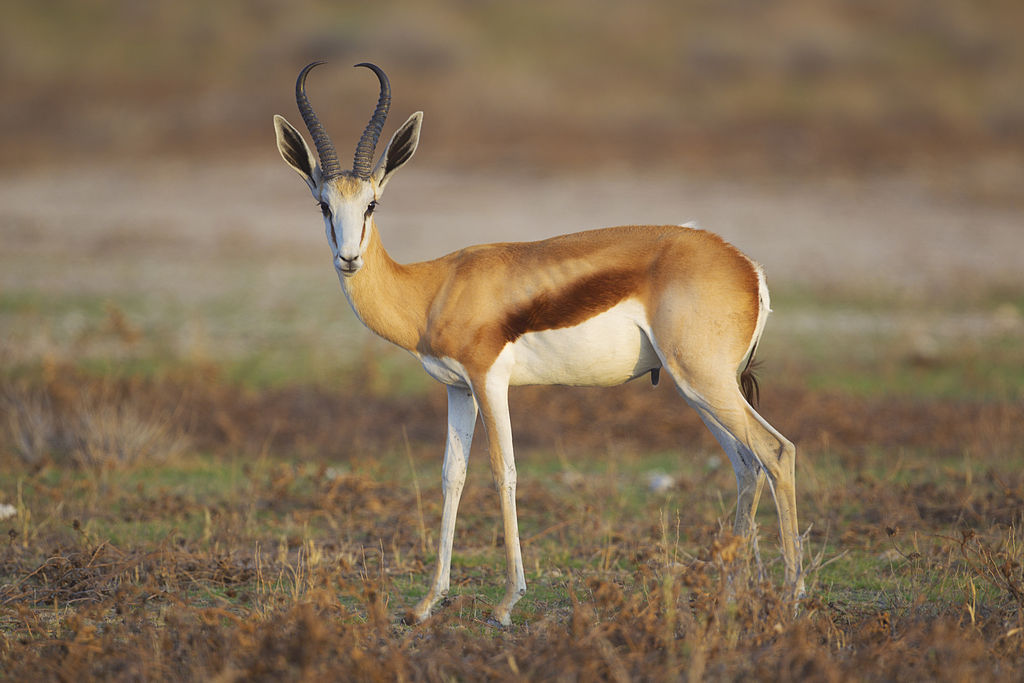
\includegraphics[width=\maxwidth{\textwidth}]{src/thesis/antidorcas.jpg}
\caption{Antidorcas marsupialis, male}
\label{figure\arabic{figurecounter}}
\legend{\emph{Source}: \iftoggle{usebiblatex}{\textcite{krishnappa_adult_2012}}{\citet{krishnappa_adult_2012}}}% See: https://upload.wikimedia.org/wikipedia/commons/8/89/Antidorcas_marsupialis%2C_male_%28Etosha%2C_2012%29.jpg
\legend{\emph{Note}: Here is a note that is especially long to show what happens when it extends to more than one line.}
\end{figure}
\refstepcounter{figurecounter}
\clearpage
\section{Math examples}

This section contains some math-heavy text adapted from \iftoggle{usebiblatex}{\textcite{dwilkins1995}}{\citet{dwilkins1995}}.
In non-relativistic wave mechanics, the wave function $\psi(\mathbf{r},t)$ of a particle satisfies the Schrödinger Wave Equation
%
\begin{equation}
 i\hbar\frac{\partial \psi}{\partial t}
  = \frac{-\hbar^2}{2m} \left(
    \frac{\partial^2}{\partial x^2}
    + \frac{\partial^2}{\partial y^2}
    + \frac{\partial^2}{\partial z^2}
  \right) \psi + V \psi.
\end{equation}
%
It is customary to normalize the wave equation by
demanding that
%
\begin{equation}
\int \!\!\! \int \!\!\! \int_{\textbf{R}^3}
      \left| \psi(\mathbf{r},0) \right|^2\,dx\,dy\,dz = 1.
\end{equation}
%
A simple calculation using the Schr\"{o}dinger wave
equation shows that
%
\begin{equation}
\frac{d}{dt} \int \!\!\! \int \!\!\! \int_{\textbf{R}^3}
      \left| \psi(\mathbf{r},t) \right|^2\,dx\,dy\,dz = 0,
\end{equation}
%
and hence
%
\begin{equation}
\int \!\!\! \int \!\!\! \int_{\textbf{R}^3}
      \left| \psi(\mathbf{r},t) \right|^2\,dx\,dy\,dz = 1
\end{equation}
%
for all times~$t$. If we normalize the wave function in this
way then, for any (measurable) subset~$V$ of $\textbf{R}^3$
and time~$t$,
%
\begin{equation}
\int \!\!\! \int \!\!\! \int_V
      \left| \psi(\mathbf{r},t) \right|^2\,dx\,dy\,dz
\end{equation}
%
represents the probability that the particle is to be found
within the region~$V$ at time~$t$.

\begin{table}[h] % Table float
\caption{This caption has math characters that remain lowercase: \relax\macrocapwrap{$\psi(\mathbf{r},t)$} }
\label{table\arabic{tablecounter}}
\begin{tabu}{l c c} \\ \hline
Column1 & Column2 & Column3 \\ \hline
Row1 & 2.0 & 3.0 \\
Row2 & 2.0 & 3.0 \\
Row3 & 7.0 & 8.0 \\ \hline
\end{tabu}
\end{table}
\refstepcounter{tablecounter}
                     %<Insert your chapters here; I recommend to use
\chapter{Problem Motivation}

\section{Introduction}    

The volume of scientific literature has doubled in the past 20 years\footnote{https://data.worldbank.org/indicator/IP.JRN.ARTC.SC}.  
The ubiquity of computing and access to free, open-source software has also enabled exponential growth in publishing for computer science fields.  
Figure \ref{figure1} shows a plot of the number of papers published on CS ArXiv\footnote{https://arxiv.org} each year 2015 to 2020 on a log scale. 

\begin{figure}[h]
    \centering
    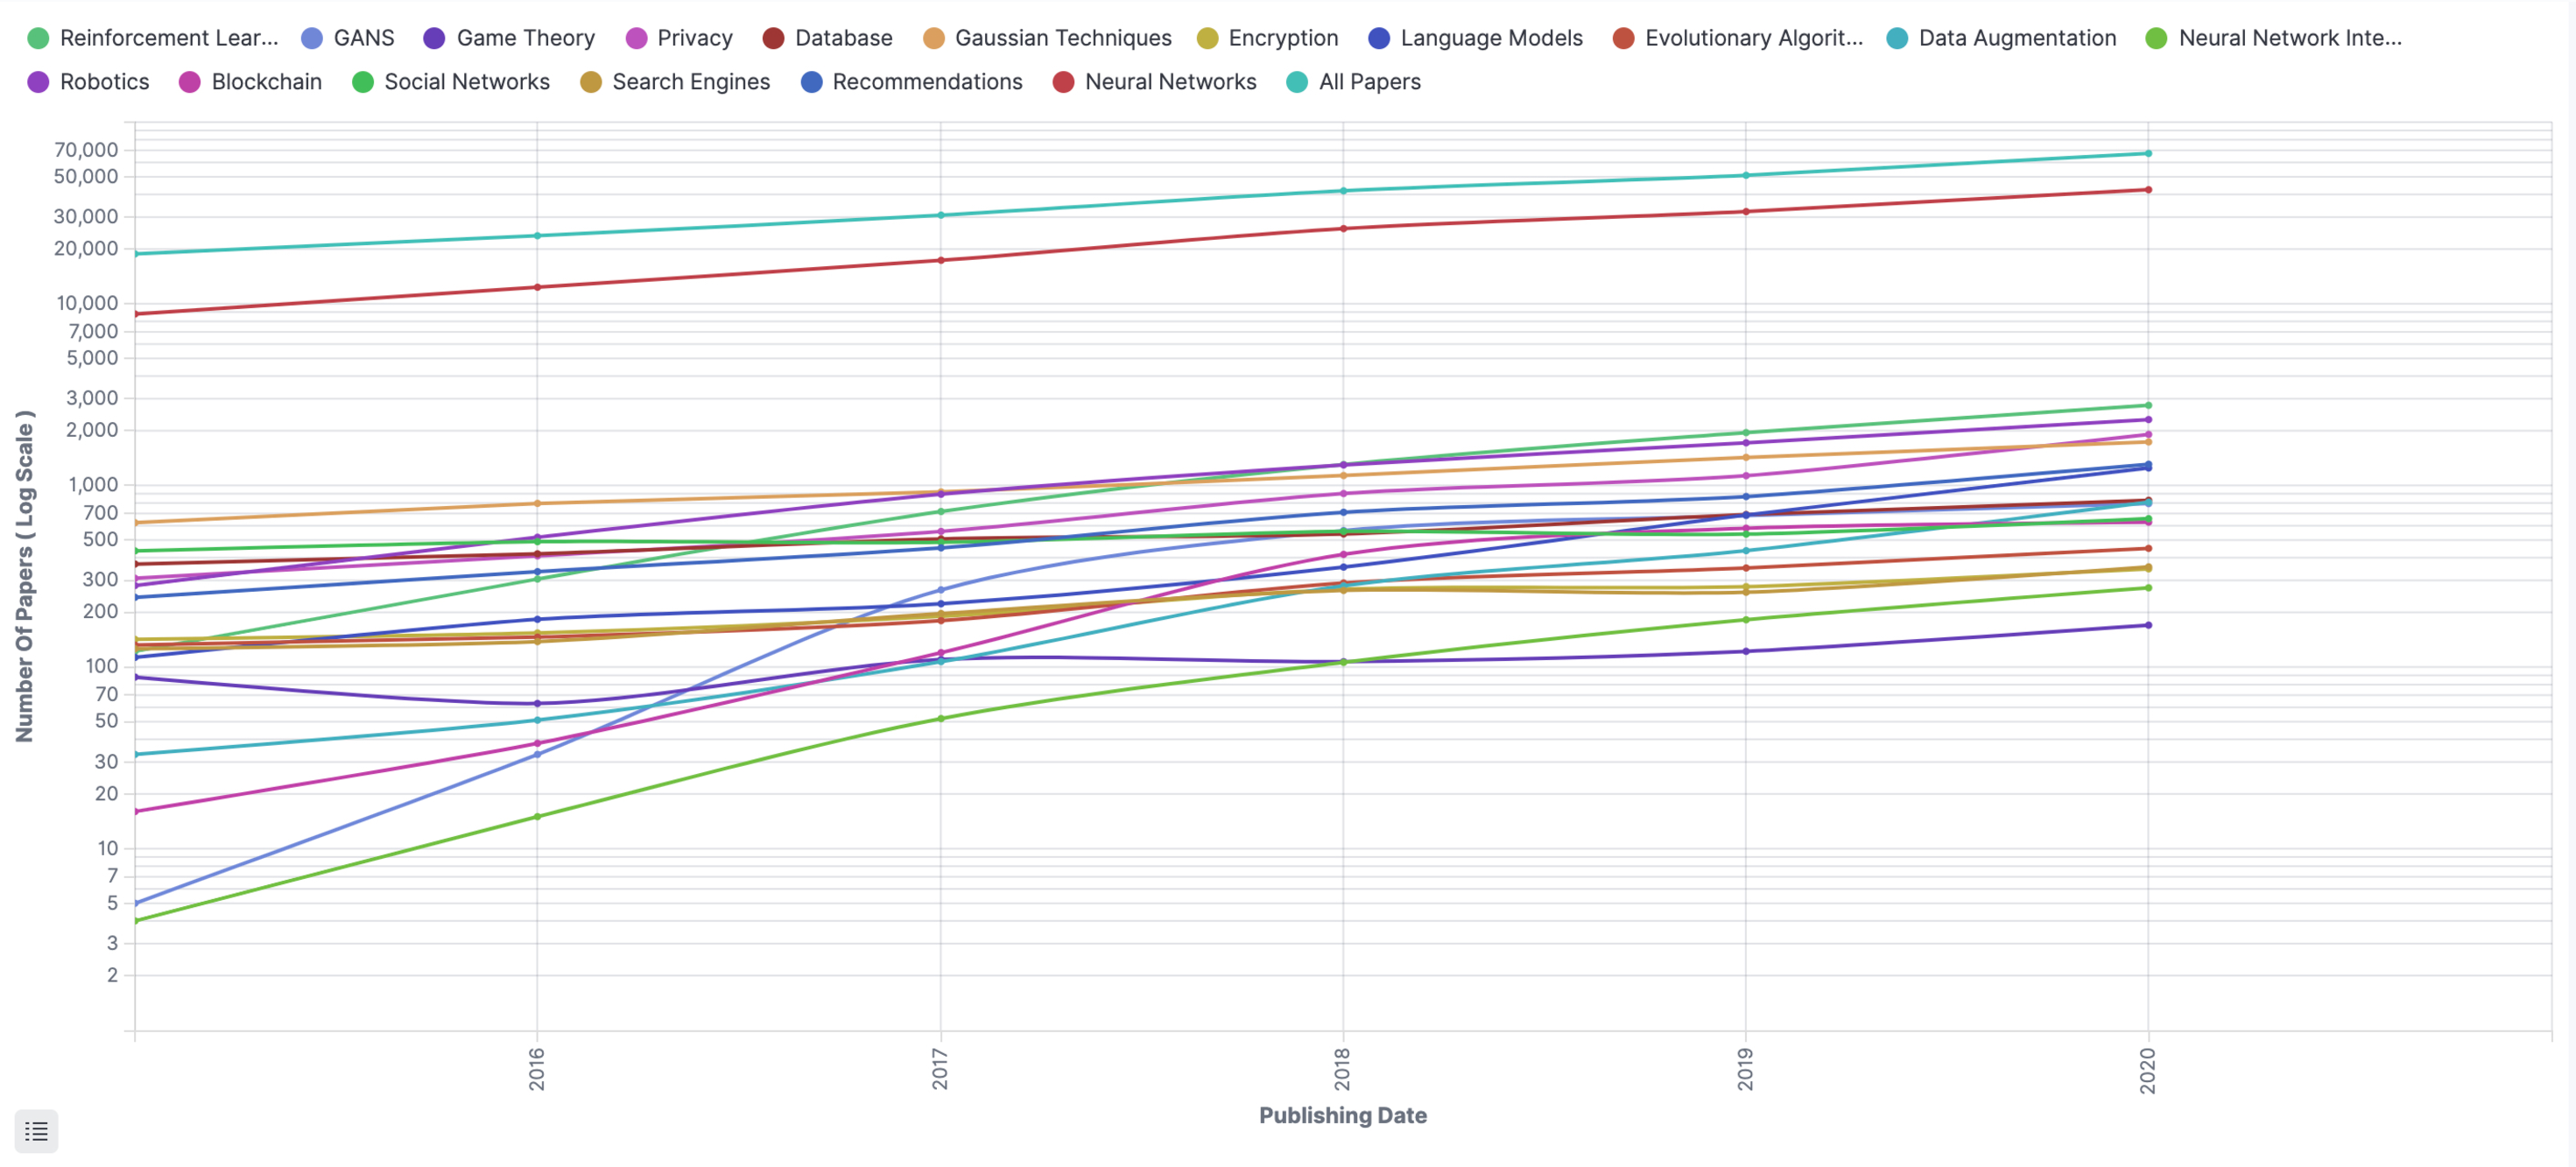
\includegraphics[width=\maxwidth{\textwidth}]{src/images/num-papers.pdf}
    \caption{ A time series plotting count of papers every year for across various topics in CS from January 2015 to December 2020}
    \label{figure\arabic{figurecounter}}
\end{figure}
\refstepcounter{figurecounter}

The growth in the research volume has also led to academic research search engines becoming primary mediums of access for scientific literature. 

Academic research search engines are different from traditional search engines like Google because they host content specific to scientific literature. 
Scientific papers generally undergo a process of peer-review. If a paper does not undergo peer review, it may still get cited by other publications/articles. This relational nature of academic research makes it relatively easy to filter credibility based on citations as a metric; Major academic research search engines such as Google Scholar, Microsoft Academic, etc., leverage citations as a metric for ranking documents. Although citations are beneficial, a search query may match many records during the search process. The increase in the number of documents can also result in a sea of noise for a particular search query. In such cases, the researcher gets minimal context information around search matches to infer why the search engine surfaced the document. 

Researchers also tend to look for information embedded deep inside papers. Many papers contain table/s of results for some experiments or comparisons to techniques/methods from other papers. This tabular information can help get on the fly context about the results/comparisons mentioned in a research paper. Such information is generally not easily accessible through normal search engines. Platforms such as PapersWithCode\footnote{https://paperswithcode.com} host/track State-of-the-art leaderboards for ML along with their papers. There are no currently available tools that augment more context about a reasearch paper when reading research. 


The next section aims to provide a motivating example to explain the lack of context in search results displayed by three large proprietary search engines.

\section{Motivating Example: Search Results From Academic Research Search Engines}
Machine Learning and deep learning research dominate most CS publications on pre-print servers like ArXiv (Figure \ref{figure1}).
Based on this information, consider the use-case of a researcher trying to look for papers where a Transformer\parencite{vaswani2017attention} model written in PyTorch\parencite{paszke2019pytorch} is given adversarial examples. 
The researcher chooses to use the following search query: \textit{pytorch transformer adversarial examples} on the search engines Google Scholar, Semantic Scholar, and Microsoft Academic. 
Ideally, the experiments or the appendix or the methodology section of a paper would consist of information about code/model in a paper. 
The following subsections will analyze the search results for this query for three large search engines: Google Scholar, Microsoft Academic, and Semantic Scholar. 
\pagebreak
\subsection{Search Results From Google Scholar}
\label{sr-g}

\begin{figure}[h]
    \centering
    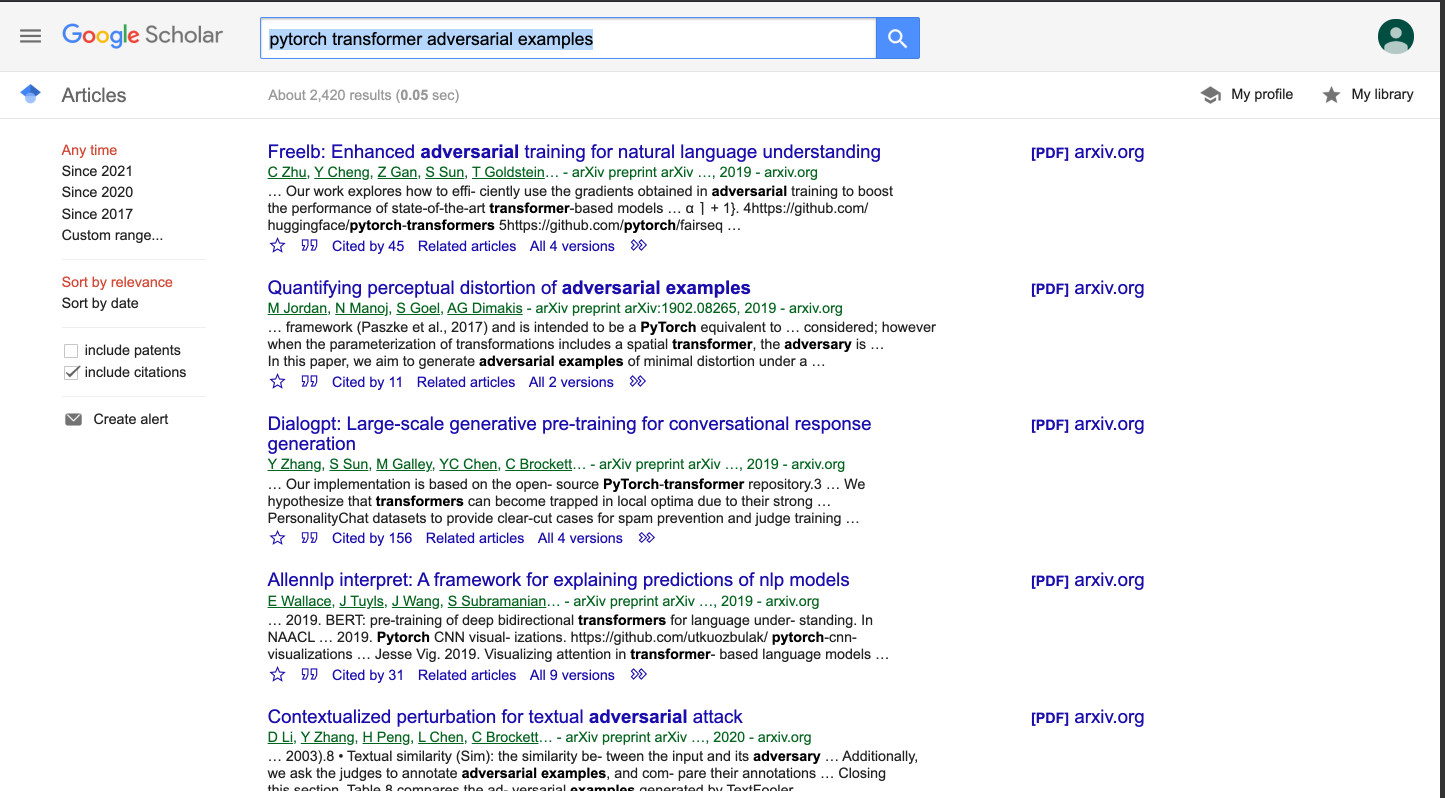
\includegraphics[width=\maxwidth{\textwidth}]{src/images/google-scholar-example.png}
    \caption{Search Results For Google Scholar}
    \label{figure\arabic{figurecounter}}
\end{figure}
\refstepcounter{figurecounter}
Although Google scholar found 2000+ search results, the search-result-fragments do not provide any additional context information about where the terms are matching.  There is no other context information except for links highlighted in the search results i.e., No mention of why the fragment matched. 

\pagebreak
\subsection{Search Results From Microsoft Academic}
\label{sr-m}
\begin{figure}[h]
    \centering
    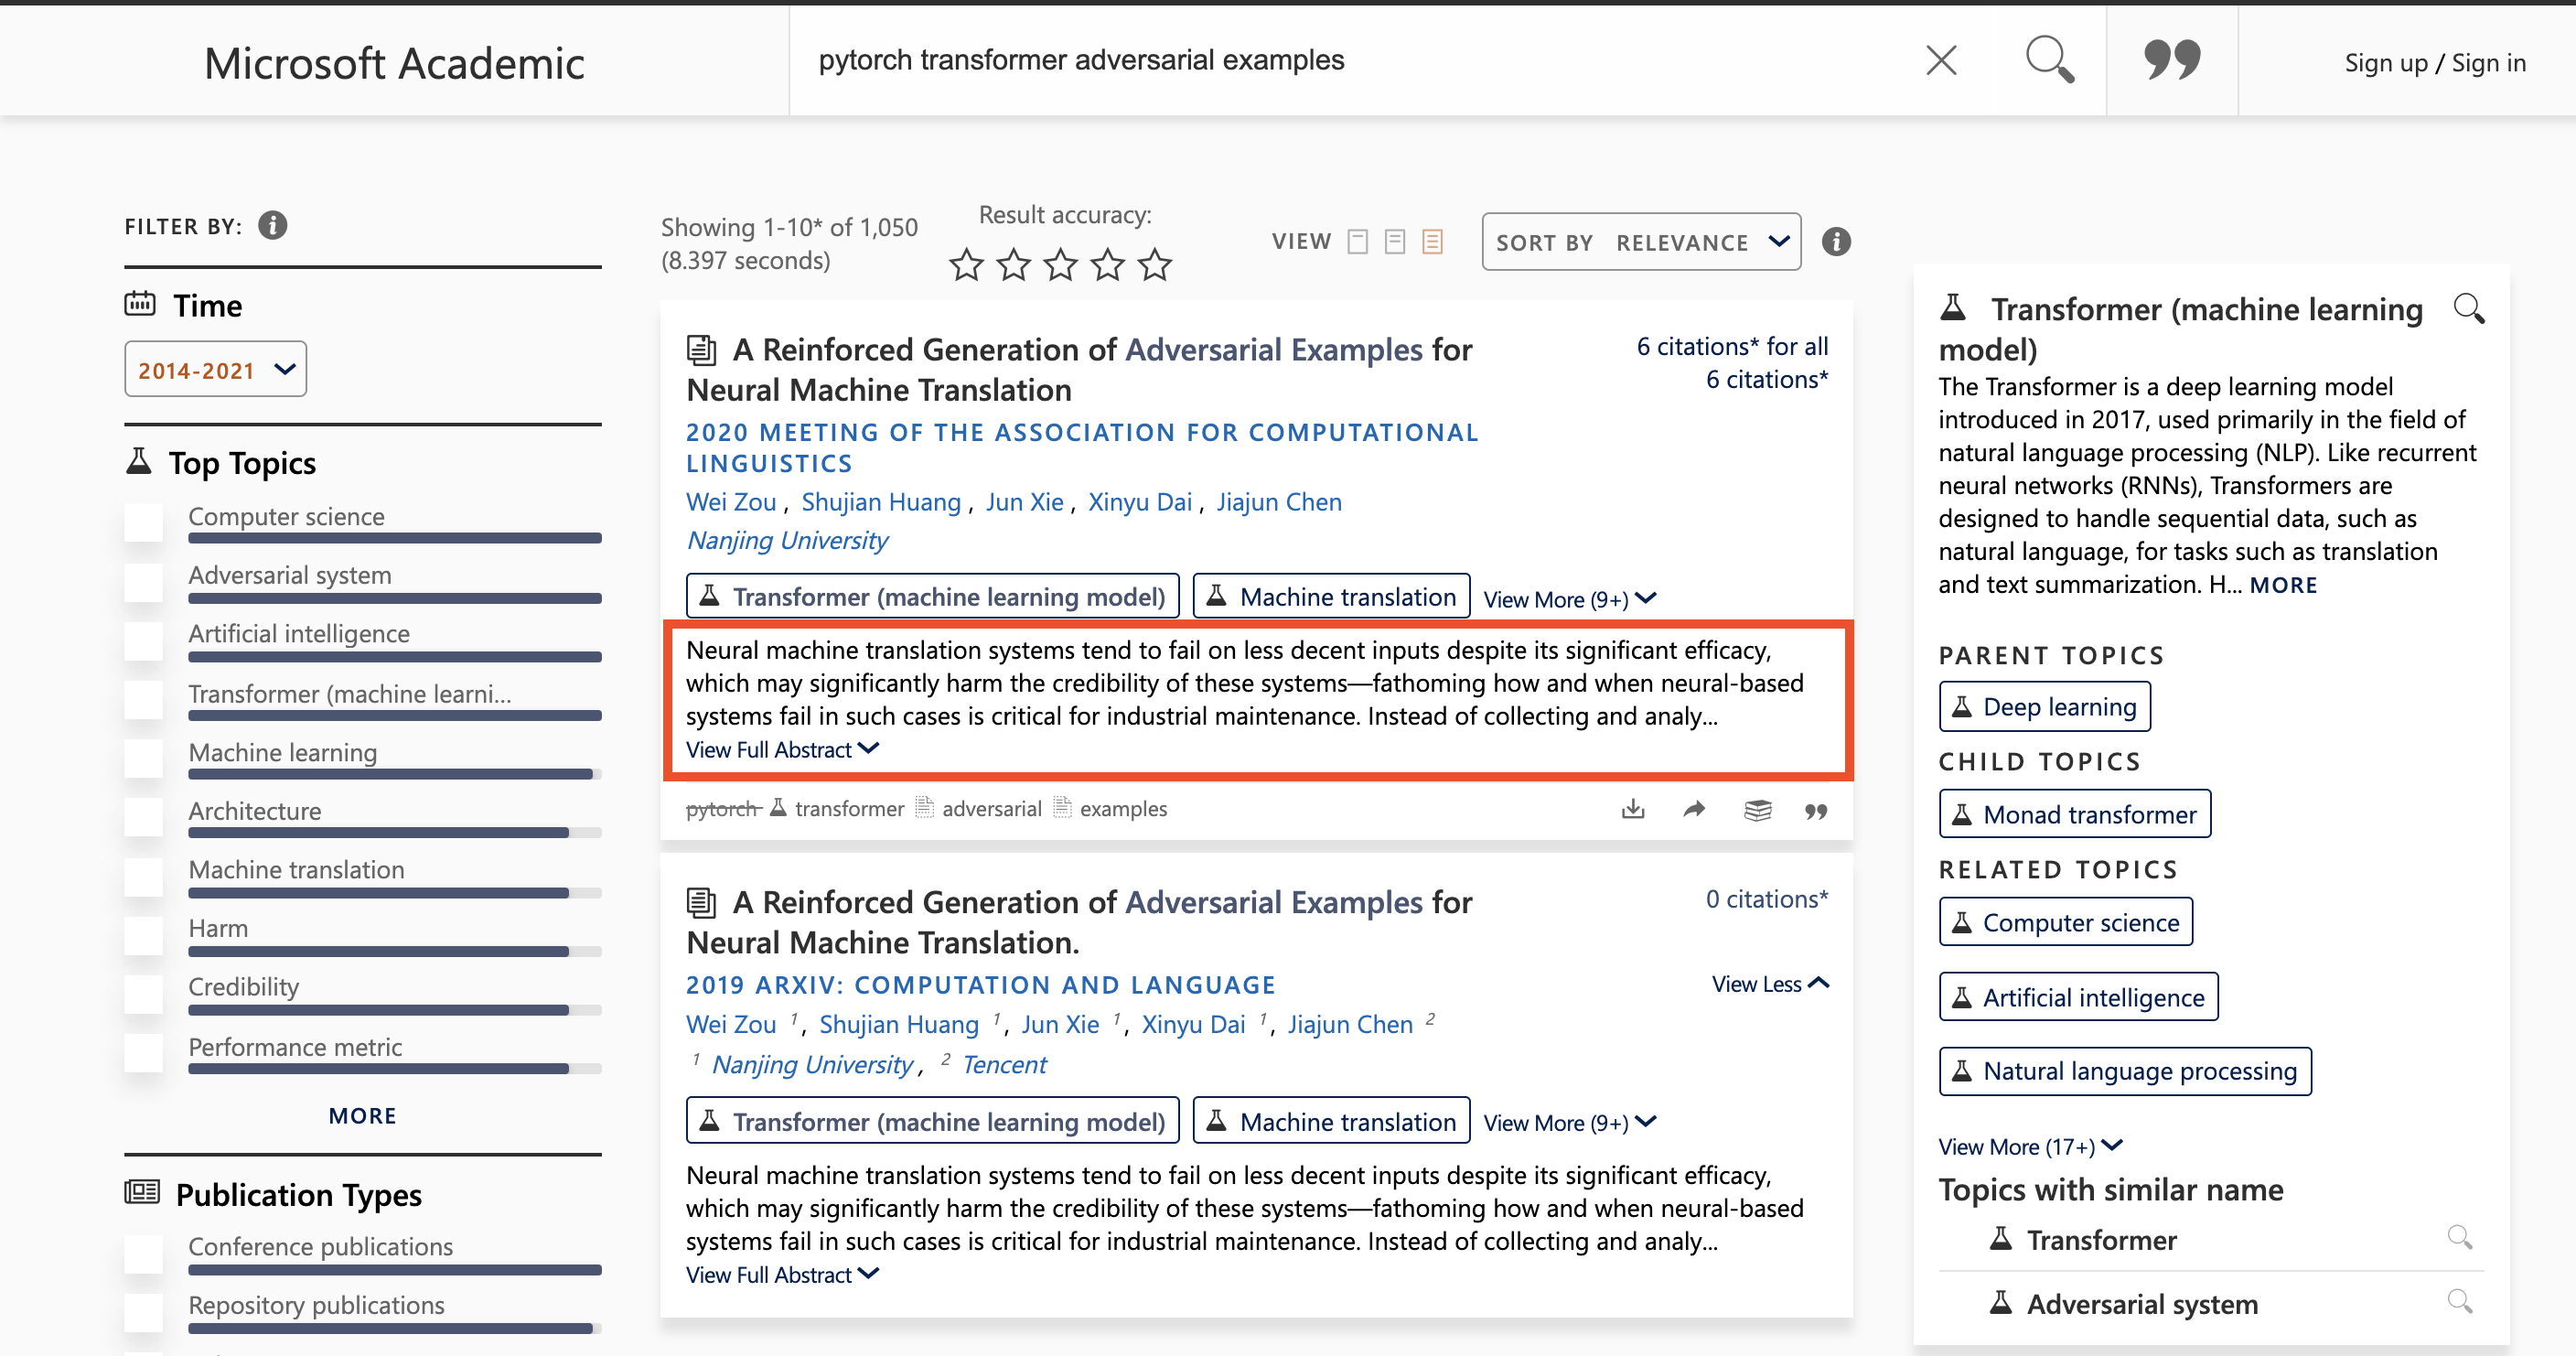
\includegraphics[width=\maxwidth{\textwidth}]{src/images/academic-example.png}
    \caption{Search Results For Microsoft Academic}
    \label{figure\arabic{figurecounter}}
\end{figure}
\refstepcounter{figurecounter}

Microsoft Academic provides additional information around context like topics, analytics on types of publication matches etc,
It fails to provide information about where the match has taken place in the paper.

\pagebreak
\subsection{Search Results From Semantic Scholar}
\label{sr-s}
\begin{figure}[h]
    \centering
    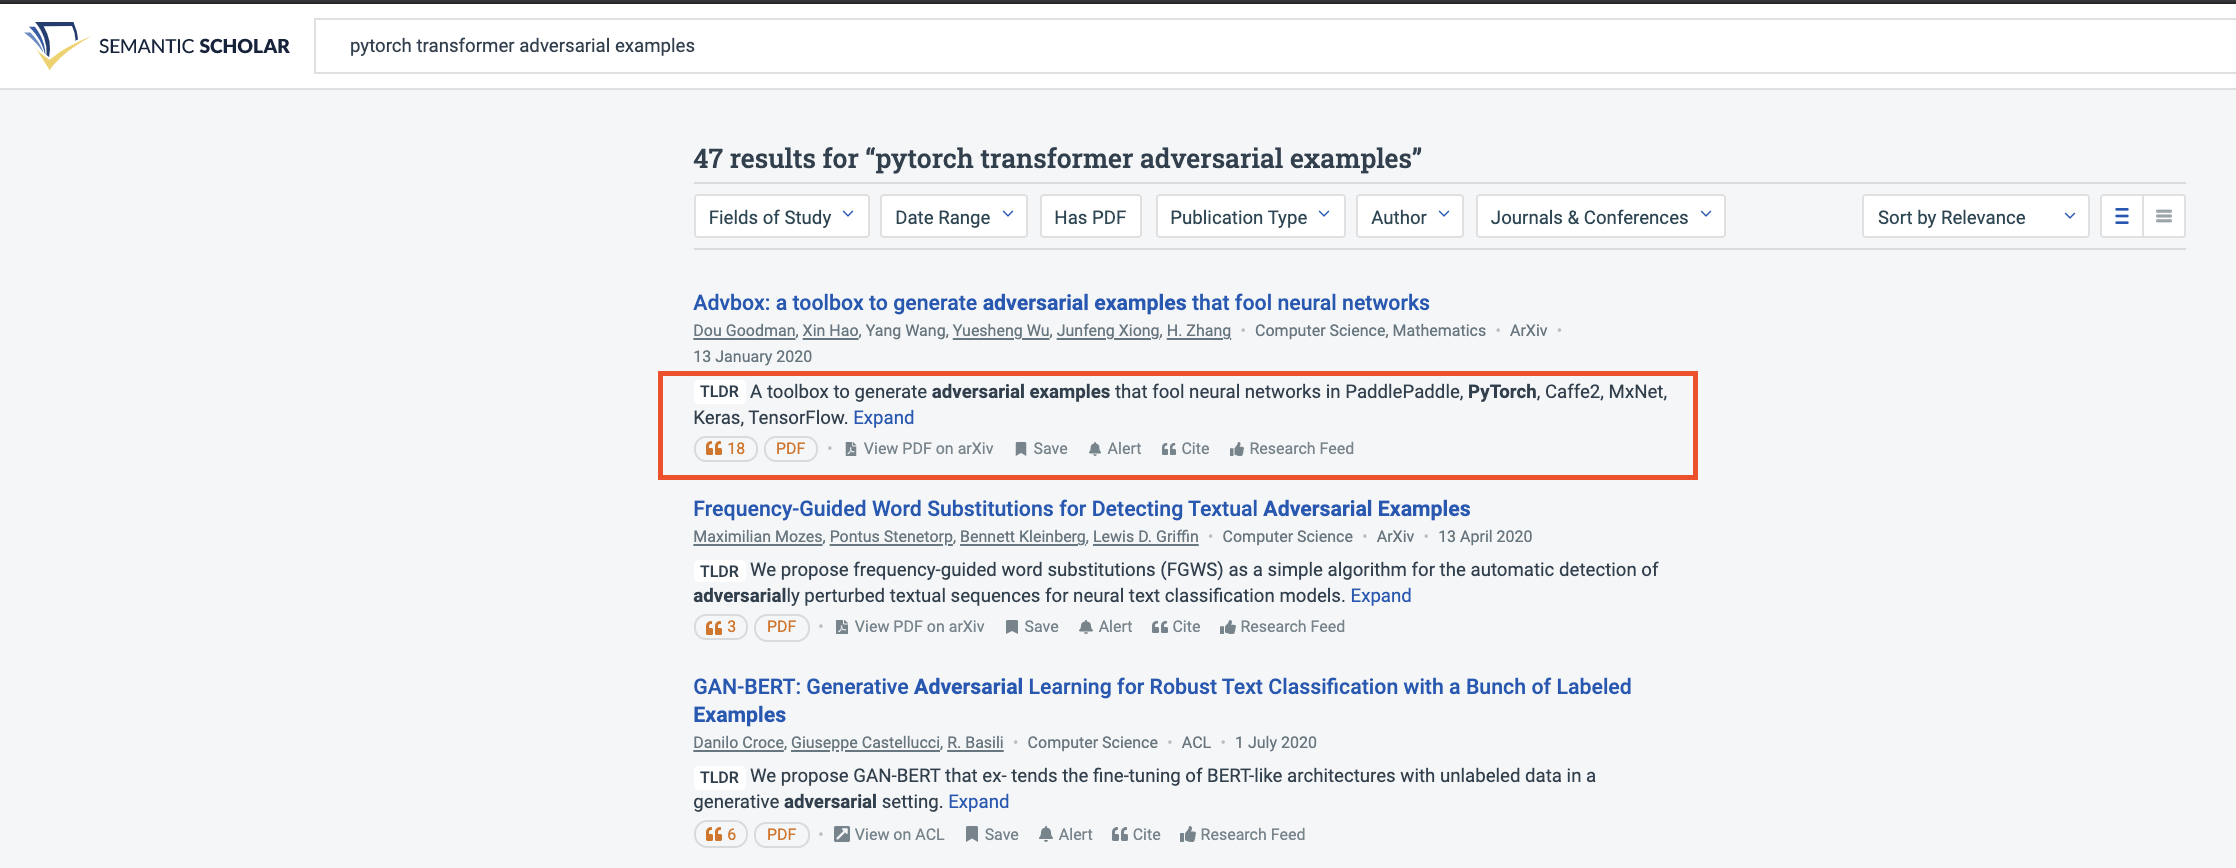
\includegraphics[width=\maxwidth{\textwidth}]{src/images/ss-example.png}
    \caption{Search Results For Semantic Scholar}
    \label{figure\arabic{figurecounter}}
\end{figure}
\refstepcounter{figurecounter}
Semantic Scholar highlights few search fragments where results would have matched and presented a smaller result set. 
But all search results do not consist of context about where the match took place. 

\pagebreak
\section{Characterizing Missing Traits}
\label{section:intro:missing_traits}

\subsection{Sparse Context In Search Results About Where Search Terms Matched Inside A Document}

All search results shown in section \ref{sr-g}, \ref{sr-m}, \ref{sr-s}, do not provide any additional information about where the match took place inside the research document. The interesting characteristic of research documents is that they possess structure and hierarchy. Research documents have well-laid out sections such as “Introduction,” “Related Works,” “Methodology,” “Experiments,” etc. that can provide context about the matched search terms. Such information can provide insights to the researcher about the context around which the search match took place. 

Previous studies by \parencite{kacem2018analysis} have shown that providing more filters to tend to improve precision in search. Access to the structure of the document can help the search engine provide filters to limit search within particular sections of a paper.

\pagebreak
\subsection{Minimal Access To Information When Reading Research}
\begin{figure}[h]
    \centering
    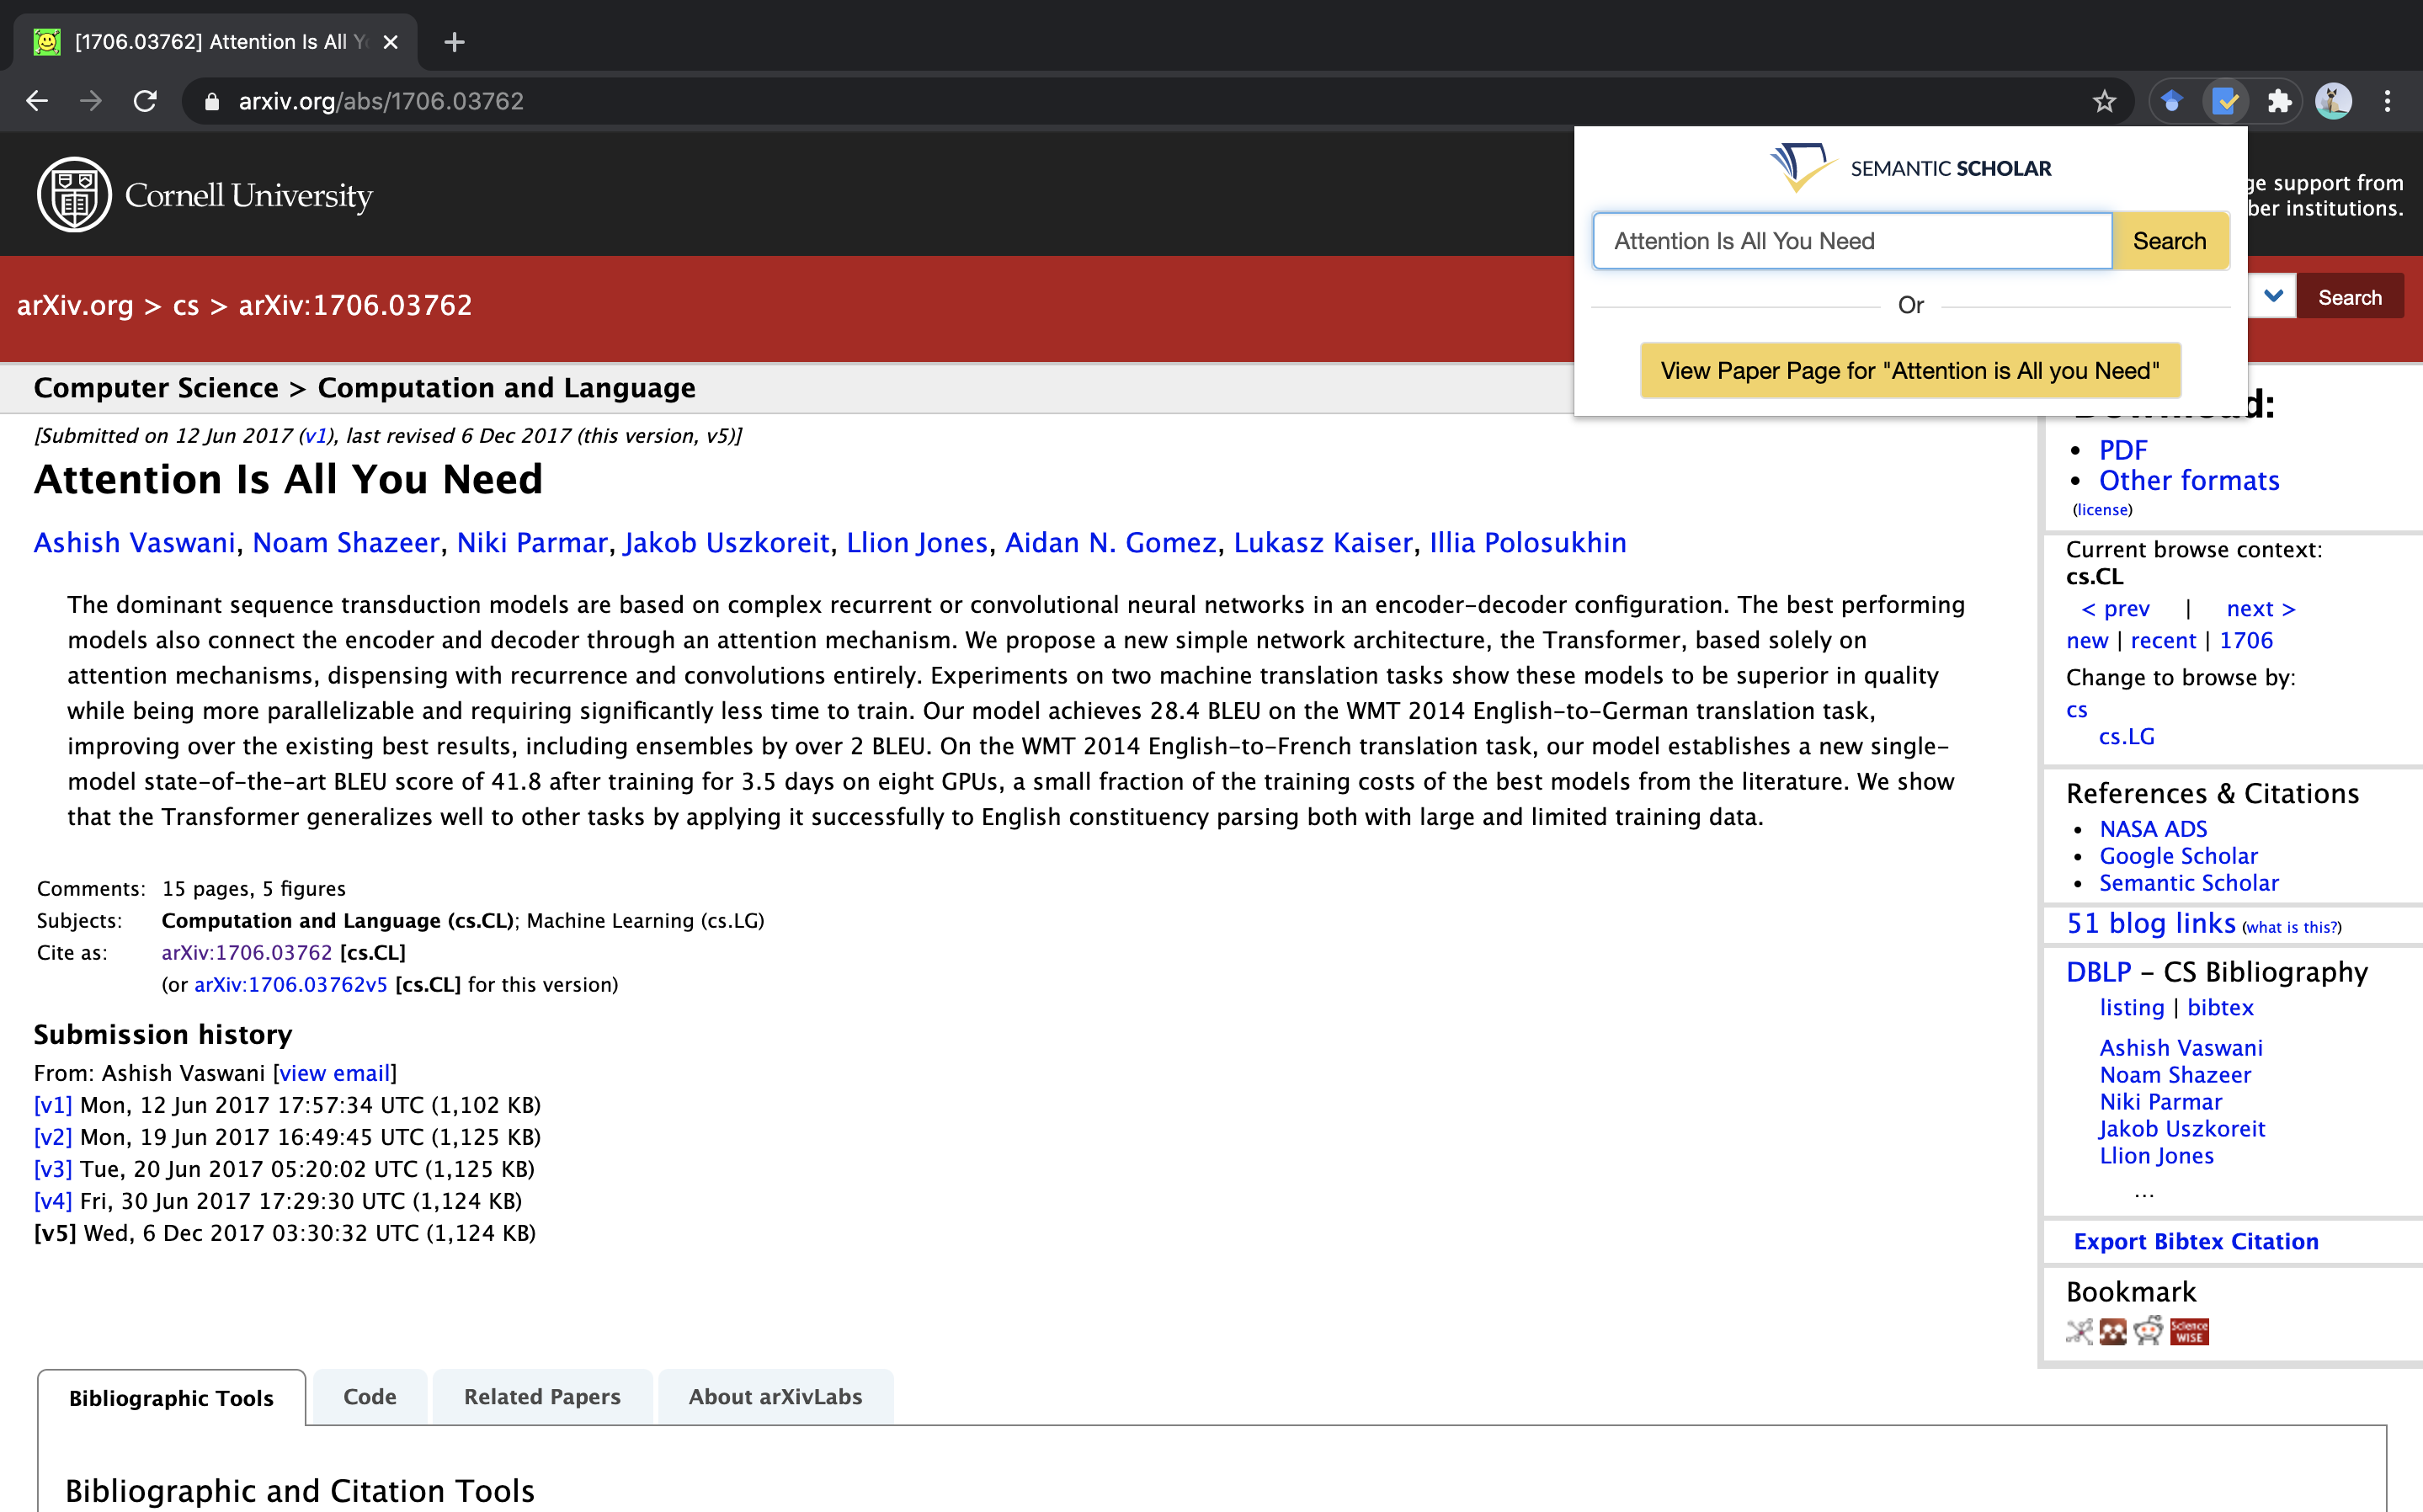
\includegraphics[width=\maxwidth{\textwidth}]{src/images/gg-plugin.png}
    \caption{Chrome(Browser) Plugin For Google Scholar}
    \label{figure\arabic{figurecounter}}
\end{figure}
\refstepcounter{figurecounter}
\begin{figure}[h]
    \centering
    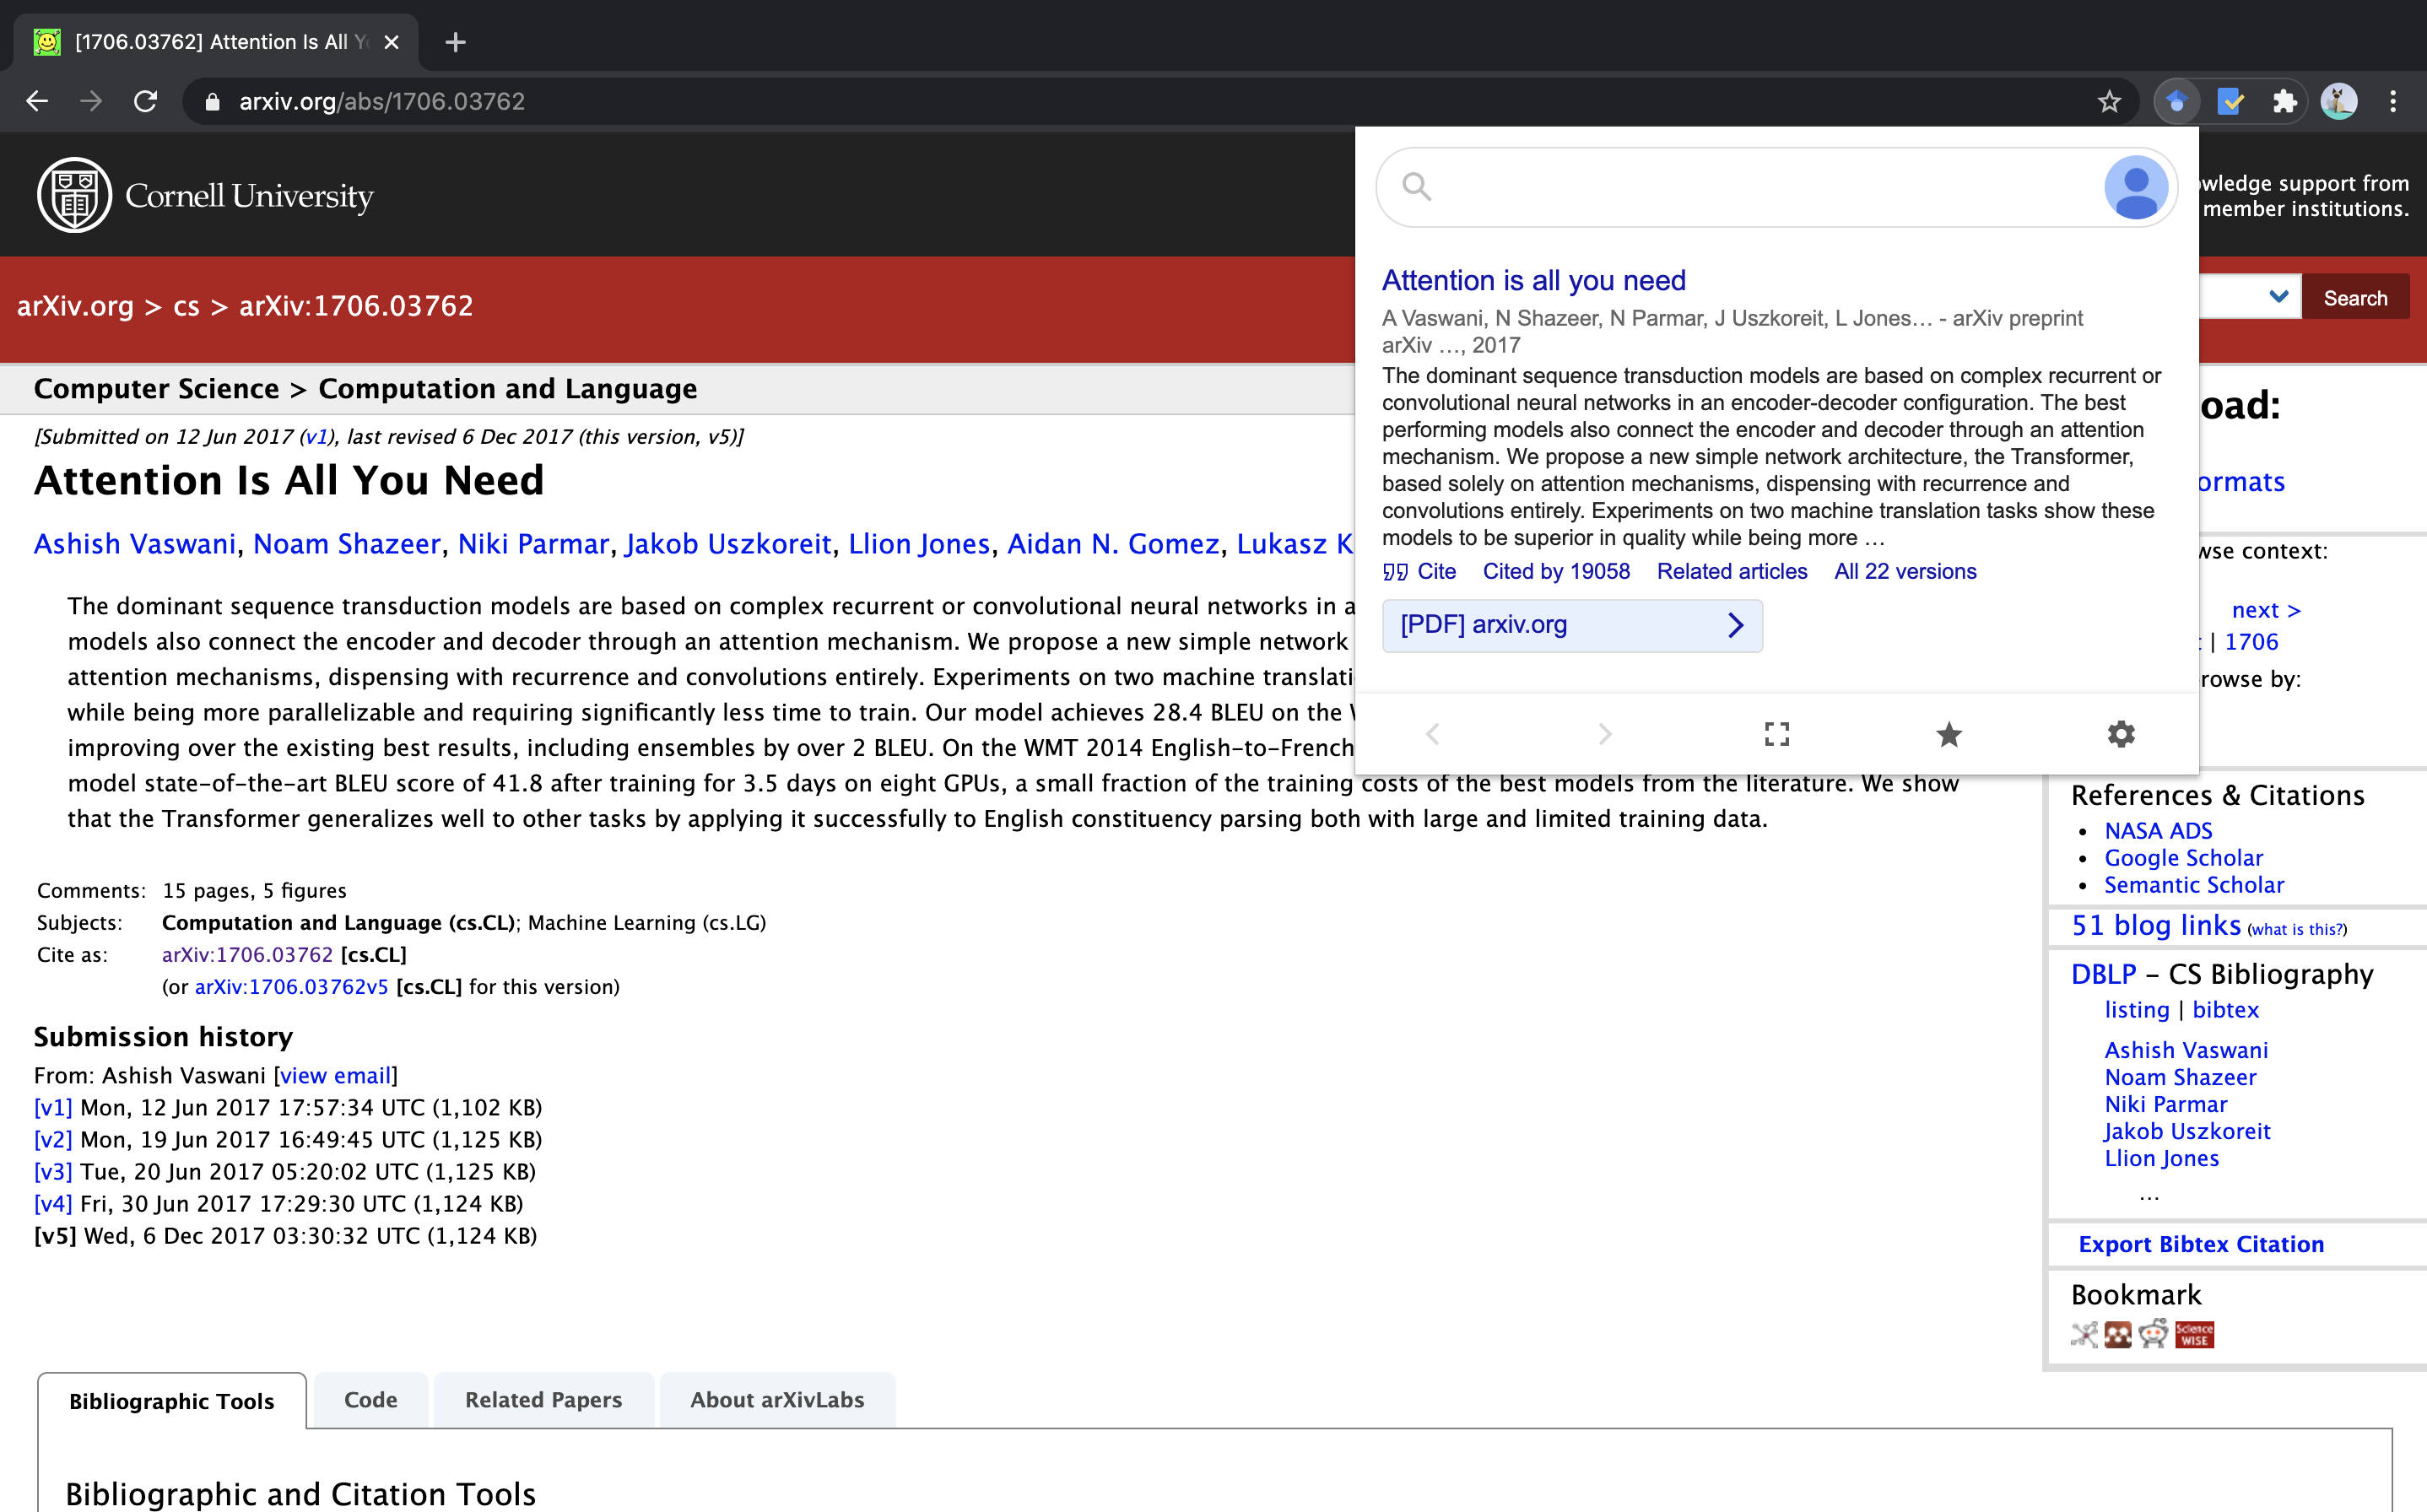
\includegraphics[width=\maxwidth{\textwidth}]{src/images/ss-plugin.png}
    \caption{Chrome(Browser) Plugin For Semantic Scholar}
    \label{figure\arabic{figurecounter}}
\end{figure}
\refstepcounter{figurecounter}
Many scientific literature search engines also offer forward citation search features, but these features are not always accessible outside the search engine’s website. 
Google Scholar and Semantic Scholar provide browser extensions to help the researchers get more context on a research document, as seen from Figure \ref{figure5} and Figure \ref{figure6}. 
These extensions lead back to the search engine's proprietary websites for further access to more information surrounding the research. They also do not provide information within the browser when the researcher is reading an article online. 
% They also miss out on many essential aspects of research documents, such as tables in the research when surfacing relevant information about the document. 
\pagebreak
\subsection{No Access To More Fine-Grained Information Such as Tables When Reading Research}

Many research papers compare methods from other research papers, and such information is not directly accessible to the researcher when reading a research article online. With the recent growth in Machine Learning publications, new platforms such as PapersWithCode\footnote{https://paperswithcode.com} and sotabench\footnote{https://sotabench.com/} help compare State-of-the-art(SOTA) methods from various research papers and link source code to many SOTA ML techniques. Even though these platforms host parsed information from raw research, there is no way to access that information when reading a research paper online. This lack of access to information results in the researcher spending valuable time finding and correlating the cited comparisons.

\section{Proposed Approach And Overview}
This dissertation focuses on the solutions developed to tackle the missing characteristics described in Section \ref{section:intro:missing_traits}. 

Section \ref{relatedwork:background} provides some preliminary background on inverted-index based search engines, open-source search engines, and state-of-the-art machine learning techniques.
Section \ref{relatedwork:acad-search-engine} discusses the different studies conducted about academic search engines; Section \ref{relatedwork:acad-lit-mining} discusses the different techniques used for mining academic literature; Section \ref{relatedwork:table-type} will discuss previous research to pertaining to classification of tables. 

Section \ref{method} provides an overview of the proposed solutions i.e., a search engine over CS ArXiv and a browser extension to augment research at the time of reading 

Section \ref{sci-genie-core} discusses the core components of the search engine and the chrome extension; Section \ref{table_classification}
discusses the problem/application/experiments for table of comparison classification task.

Finally, Section \ref{conclusion} will provide some insight to the current shortcomings of Sci-Genie and highlight some future directions based on the shortcomings of Sci-Genie  
% \include{src/thesis/background}                     %<Insert your chapters here; I recommend to use
\chapter{Related Works}
\label{relatedwork}

\section{Background Literature}
\label{relatedwork:background}

\subsection{Lucene Based Inverted Search Index}
An inverted index lists every unique word in any document and identifies all the documents each word occurs in. Since the late 1990s, search engines have been using an inverted index as the core structure to store and access information; Even Google, in its earlier stages, leveraged inverted indexes as means of accessing text documents for search\parencite{brin1998anatomy}. Sergey Brin and Larry Page partitioned web search engines to perform three critical tasks: Parsing, Indexing, and Ranking.

Opensource search engines such as the Apache Lucene\parencite{lucene2010apache} help provide hooks to index and rank documents for search. Lucene has become a popular search engine as many open-source search engines are built on top of Lucene to help simplify the access of the features of Lucene. Solr\footnote{https://solr.apache.org/}, Elasticsearch\footnote{https://www.elastic.co/elasticsearch/} as some opensource search engines built on top of Lucene. 

\subsubsection{Indexing With Lucene}
As Lucene leverages an inverted index to store information, it defines two fundamental units for indexing:
\begin{itemize}
    \item Document : A container for various Fields
    \item Field : Stores the terms that need to be indexed. It is key-value form of mapping. 
\end{itemize}
The Document allows for storing large hierarchical tree-like structures when indexing JSON objects. Every index consists of Documents. The index is similar to Database in the language of RDBMS. 

\subsection{Transformers and Machine Learning SOTA}
The Transformer model \parencite{vaswani2017attention} has recently proven to show SOTA performance on various domains ranging from natural language \parencite{brown2020language}, vision(\cite{radford2021learning}, \cite{dosovitskiy2020image}), music \parencite{huang2018music}, image-generation \parencite{ramesh2021zero} and even Web Table mining \parencite{deng2020turl}. These models can be trained with large amounts of data using self supervised training objectives \parencite{chen2020big}, \parencite{kolesnikov2019revisiting}, \parencite{goyal2019scaling}, \parencite{gidaris2018unsupervised}, \parencite{doersch2015unsupervised}. Once trained, these models can transfer their learning to different downstream tasks by making minor adjustments to their weights \parencite{howard2018universal} based on the task.  

\subsubsection{Transformer Architecture}
\begin{figure}[h]
    \centering
    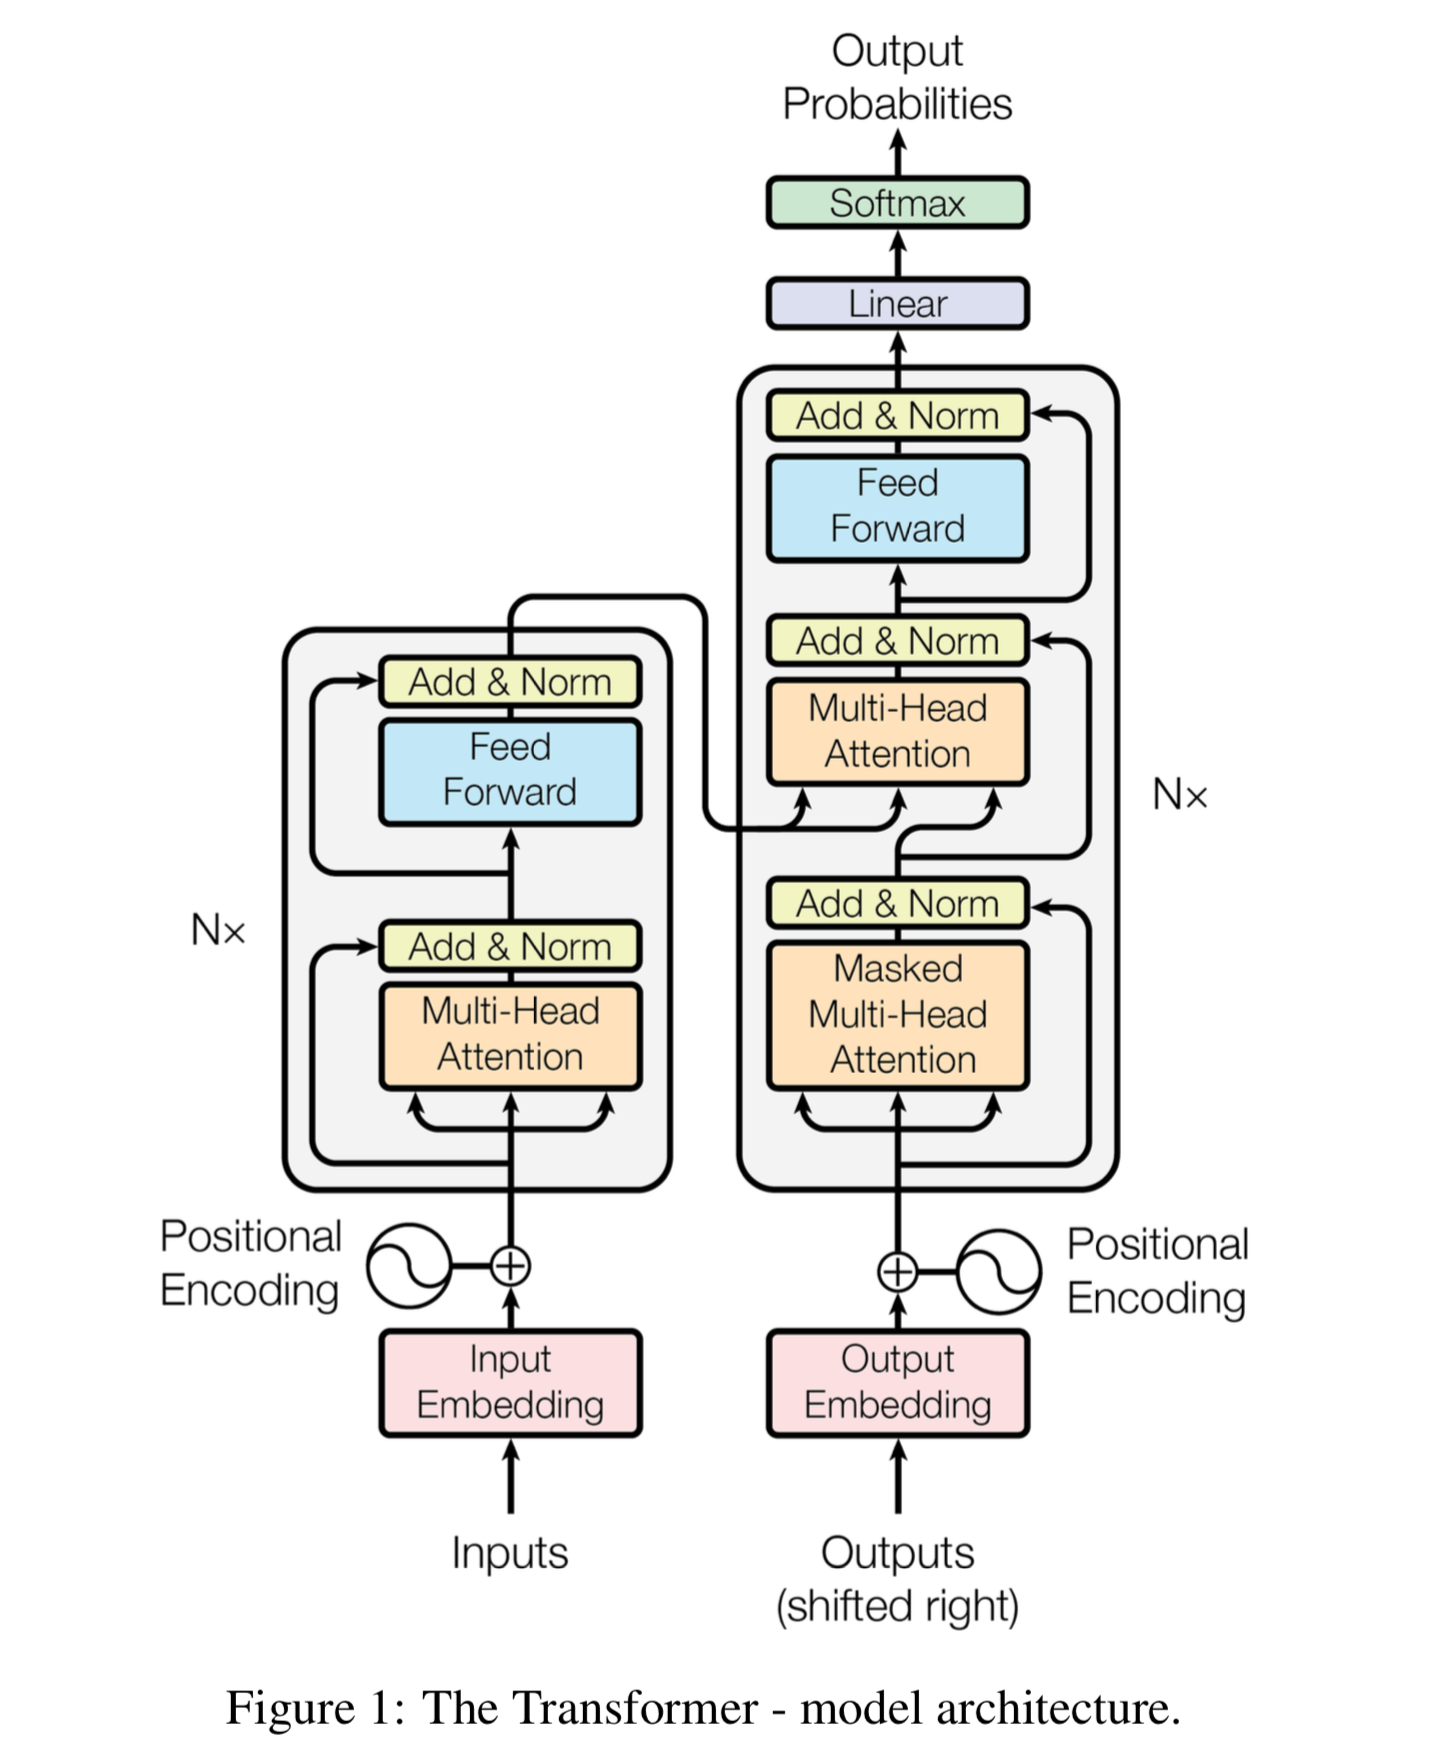
\includegraphics[width=0.7\maxwidth{\textwidth}]{src/images/transformer.png}
    \legend{\emph{Source}: From \cite{vaswani2017attention}}
    \caption{Transformer Architecture}
    \label{figure\arabic{figurecounter}}
\end{figure}
\refstepcounter{figurecounter}

The vanilla Transformer architecture \parencite{vaswani2017attention} was created for machine translation. The model consisted of an Encoder-Decoder Architecture using self-attention/cross-attention layers. The input to the transformer requires a sequence of symbols. The sequence of input and target symbols are created via a word piece tokenizer. The tokenized sequences are transformed into sequences of embeddings. Positional embeddings are added to the sequences, and then they are passed through either the encoder or decoder layer.

The self-attention/cross-attention layers consist of a multiheaded self-attention/cross-attention operation followed by pointwise feedforward layers with batch normalization \parencite{ioffe2015batch} and residual connections \parencite{he2016deep}. Multiple such layers are stacked together to create an encoder or decoder of the transformer. 

The encoder layer encodes a sequence into latent representations using the self-attention operation; the decoder layer decodes the latent representation from the encoder with the cross attention for language translation. Figure \ref{figure7} visualizes the operation of the encoder and decoder. 

Multiple variants of this architecture have been created such as the ones by \cite{radford2019language}, \cite{devlin2018bert}. The key insight behind the attention operation is provided in Section \ref{relatedwork:background:transformer:attention}, Section \ref{relatedwork:background:transformer:cross-attention}, 

\paragraph{Self-Attention}
\label{relatedwork:background:transformer:attention}
The self attention operation operates on a sequence $S \in \mathbb{R}^{s \times d}$ of $s$ length and $d$ dimensions. The self attention operation comprises three key components. A key matrix $K$, A query matrix $Q$, and value matrix $V$;each created from a linear transformation of $S$. 
$$A = softmax(\frac{QK^T}{\sqrt{d}})V$$

The $softmax(\frac{QK^T}{\sqrt{d}})$ operation creates a $s \times s$ dimensional matrix. Element ${i,j}$ in the matrix correspond to the weight of index $i$ in the sequence $S$ to index $j$ in sequence $S$. The operation is called self attention because the key matrix and the query matrix are derived from same sequence.

\paragraph{Cross Attention}
\label{relatedwork:background:transformer:cross-attention}
Self attention operation applies the attention opperation over the same sequence; Cross attention applies the attention operation over different sequences. The cross attention operates on a sequence $S_\alpha \in \mathbb{R}^{s \times d}$ and $S_\beta \in \mathbb{R}^{k \times d}$ where $S_\alpha$ is of $s$ length and $d$ dimensions and $S_\beta$ is of $k$ length and $d$ dimensions. The query matrix $Q_\alpha$ is created from a linear transformation of $S_\alpha$ and key matrix $K_\beta$, value matrix $V_\beta$ are created from a linear transformation of $S_\beta$. 

$$A_\alpha=softmax(\frac{Q_{\alpha}K_{\beta}^{T}}{\sqrt{d}})V_{\beta}$$

The $softmax(\frac{Q_{\alpha}K_{\beta}^{T}}{\sqrt{d}})$ operation creates a $s \times k$ dimensional matrix. Element ${i,j}$ in the matrix correspond to the weight of index $i$ in the sequence $S_\alpha$ to index $j$ in sequence $S_\beta$. This operation is useful in tasks such as language translation where the $S_\alpha$ can be a source language sentence and $S_\beta$ can be the target language sentence for translation.  

\subsubsection{Pretraining and Self Supervised Learning}
In NLP, Transformer models possess properties to scale and learn with massive amounts of data using generalized tasks such as language modeling or masked language modeling. The objective of language modeling is to predict the token $n+1$ given $n$ tokens in the sequence. The masked language modeling objective is to predict a masked out token in the sequence correctly given the other tokens. These training objectives allow the usage of large amounts of data from the web without going through the effort to clean the data. Recent State-of-the-art Language models such as GPT-3 \parencite{brown2020language} are trained using such self-supervised training objectives. 

\subsubsection{Advantages To Transfer Learning After Pretraining Models}
Recent studies such as the one by \cite{hernandez2021scaling}, showed that transformer models pretrained on large data with self-supervised learning objectives transfer learn better to downstream tasks with much less labeled data. The finetuning step\parencite{howard2018universal} of transfer learning involves adding a new linear layer and then training the model with small learning rates for the task-specific optimization. 


\subsubsection{Machine Learning For Tabular Data}
\cite{deng2020turl} recently applied structurally aware Transformers for self-supervised learning of web tables. The learned models possessed rich generalization capabilities for transfer into downstream tasks such as row filling based on headers, Entity Linking to the knowledge base, column type annotation etc. 

\section{Academic Research Search Engines}
\label{relatedwork:acad-search-engine}
\cite{gusenbauer2020academic} conducted an analysis of search engines based on criteria described in Table \ref{table1}.
The criteria described by \cite{gusenbauer2020academic} try to objectively evaluate the usefulness of a search engine to do systematic reviews.

\begin{table*}[h]
    \label{table\arabic{tablecounter}}
    \csvreader[%
     tabular={|p{7cm}|p{10cm}|},
            table head = \hline\textbf{Criteria} & \textbf{Meaning} \\\hline,
            late after line= \\\hline,
            late after last line=\\\hline %
            ]{searching-criteria-0.csv}{Criteria=\Criteria,Meaning=\Meaning}%
            {\Criteria & \Meaning}
            \centering
            \legend{\emph{Source}: From \cite{gusenbauer2020academic}}
            \caption{\label{tablecounter}Table explaining various criteria For Comparing Search Engines}
\end{table*}
\refstepcounter{tablecounter}

\begin{table*}[h]
    \label{table\arabic{tablecounter}}
    \csvreader[%
     tabular={|p{7cm}|p{10cm}|},
            table head = \hline\textbf{Criteria} & \textbf{Meaning} \\\hline,
            late after line= \\\hline,
            late after last line=\\\hline %
            ]{searching-criteria-1.csv}{Criteria=\Criteria,Meaning=\Meaning}%
            {\Criteria & \Meaning}
            \centering
            \legend{\emph{Source}: From \cite{gusenbauer2020academic}}
            \caption{\label{tablecounter}Table explaining various criteria for comparing search engines}
\end{table*}
\refstepcounter{tablecounter}

\begin{table*}[h]
    \label{table\arabic{tablecounter}}
    \csvreader[%
     tabular={|p{7cm}|p{10cm}|},
            table head = \hline\textbf{Criteria} & \textbf{Meaning} \\\hline,
            late after line= \\\hline,
            late after last line=\\\hline %
            ]{searching-criteria-2.csv}{Criteria=\Criteria,Meaning=\Meaning}%
            {\Criteria & \Meaning}
            \centering
            \legend{\emph{Source}: From \cite{gusenbauer2020academic}}
            \caption{\label{tablecounter}Table explaining various criteria for comparing search engines}
\end{table*}
\refstepcounter{tablecounter}

% Recent studies have tried to compare various search engines, finding causes for search failures and 
% recommend feature to improve search precision. 


\cite{li2017investigating} performed a detailed analysis on the patterns and failures in search for academic search. 
Their analysis concluded that search queries in academic search had substantially more entity-based queries than web search and 
null queries attributed to a significant fraction of failures, i.e., search engine found no search results. 
This analysis is quite helpful in correlating the need for a "Controlled Vocabulary"(Table \ref{table1}) in search to improve precision. 

\cite{kacem2018analysis} analyzed the improvement of search precision based on the usage of \textit{search stratagems}.
Search stratagems are additional filters along with the search terms. They provide further context around filtering a search query. 
Some examples of such filters can Authors of a paper, Forward Citation Search, Footnote Chasing, etc.
The study by \cite{kacem2018analysis} concluded that search stratagems could improve search precision for the search queries.

\cite{rovira2019ranking} conducted a study to analyze the impact of citation count on ASEO(Academic Search Engine Optimization). 
Their study concluded that Microsoft Academic and Google Scholar seem to leverage received citations as a part of the relevance 
ranking algorithm. This study also noted many unknown attributes in the relevance ranking algorithms for Google Scholar and Microsoft Academic.


\section{Academic Research Literature Mining}
\label{relatedwork:acad-lit-mining}
Academic Literature mining has many applications such as document structure analysis, citation analysis, document summarization, table extraction, and more. Deep learning-based methods dominate many of the recent SOTA academic literature mining methods. 

\cite{beltagy2019scibert} created Sci-Bert by training a BERT model \parencite{devlin2018bert} using a large corpus of research data. Sci-Bert can be finetuned for downstream tasks such as citation intent detection, relation extraction, and even named entity detection. 
 
\cite{safder2020deep} leveraged deep learning techniques extract metadata from research documents. \cite{zha2019mining} proposed methods to track the evolution of algorithms and techniques to make research more understandable. 

Table extraction and parsing have also seen a lot of recent advancements. Methods either work on PDF-based documents or LaTeX based documents.  Some such advances can include \cite{milosevic2019framework}'s framework for extracting tables from biomedical literature articles or \cite{kardas2020axcell}'s methods for extracting tables describing SOTA comparisons from machine learning papers. 

All of these advances are because of curation and opensource availability to many datasets some of such being Arxiv Tables\footnote{http://boston.lti.cs.cmu.edu/eager/table-arxiv/} or Semantic Scholar Open Research Corpus\parencite{ammar-etal-2018-construction} or the Sci-Cite dataset \parencite{cohan2019structural} or the PaperWithCode datasets\footnote{https://paperswithcode.com/}.


\section{Types Of Tables in Scientific Research}
\label{relatedwork:table-type}
Earlier work done by \cite{kim2012scientific} defined the types of tables based on their content and purpose. \cite{kim2012scientific} sampled 25 papers from the domains of CS, Biomedical, Life Science, Chemistry, Material Science, Electrical Engineering and Medicine chose to define the following types of tables for scientific documents:
\begin{itemize}
    \item \textbf{Definition Table} : \textit{These tables describe equation definitions or symbol definitions}
    \item \textbf{Statistics Table} : \textit{These tables describe some statistical distribution which is not related to experiment results}
    \item \textbf{Survey Table } : \textit{These tables describe questionaire surveys and results }
    \item \textbf{Example Table } : \textit{These tables provide emphasis of something that needs to be clearly explained }
    \item \textbf{Procedure Table} : \textit{These tables describe a flow or a process}
    \item \textbf{Experiments Setting Table } : \textit{These tables describe some experiment parameters}
    \item \textbf{Experiments Results Table } : \textit{These tables describe the results of some experiments discussed in the paper.}
\end{itemize}

\cite{kim2012scientific} also found that most of the tables in scientific documents describe results from experiments based on the samples they annotated. 




\chapter{Proposed Solutions}
\label{method}

\section{Sci-Genie : Search Engine Harnessing Structure Of Scientific Research}
\begin{figure}[h]
    \centering
    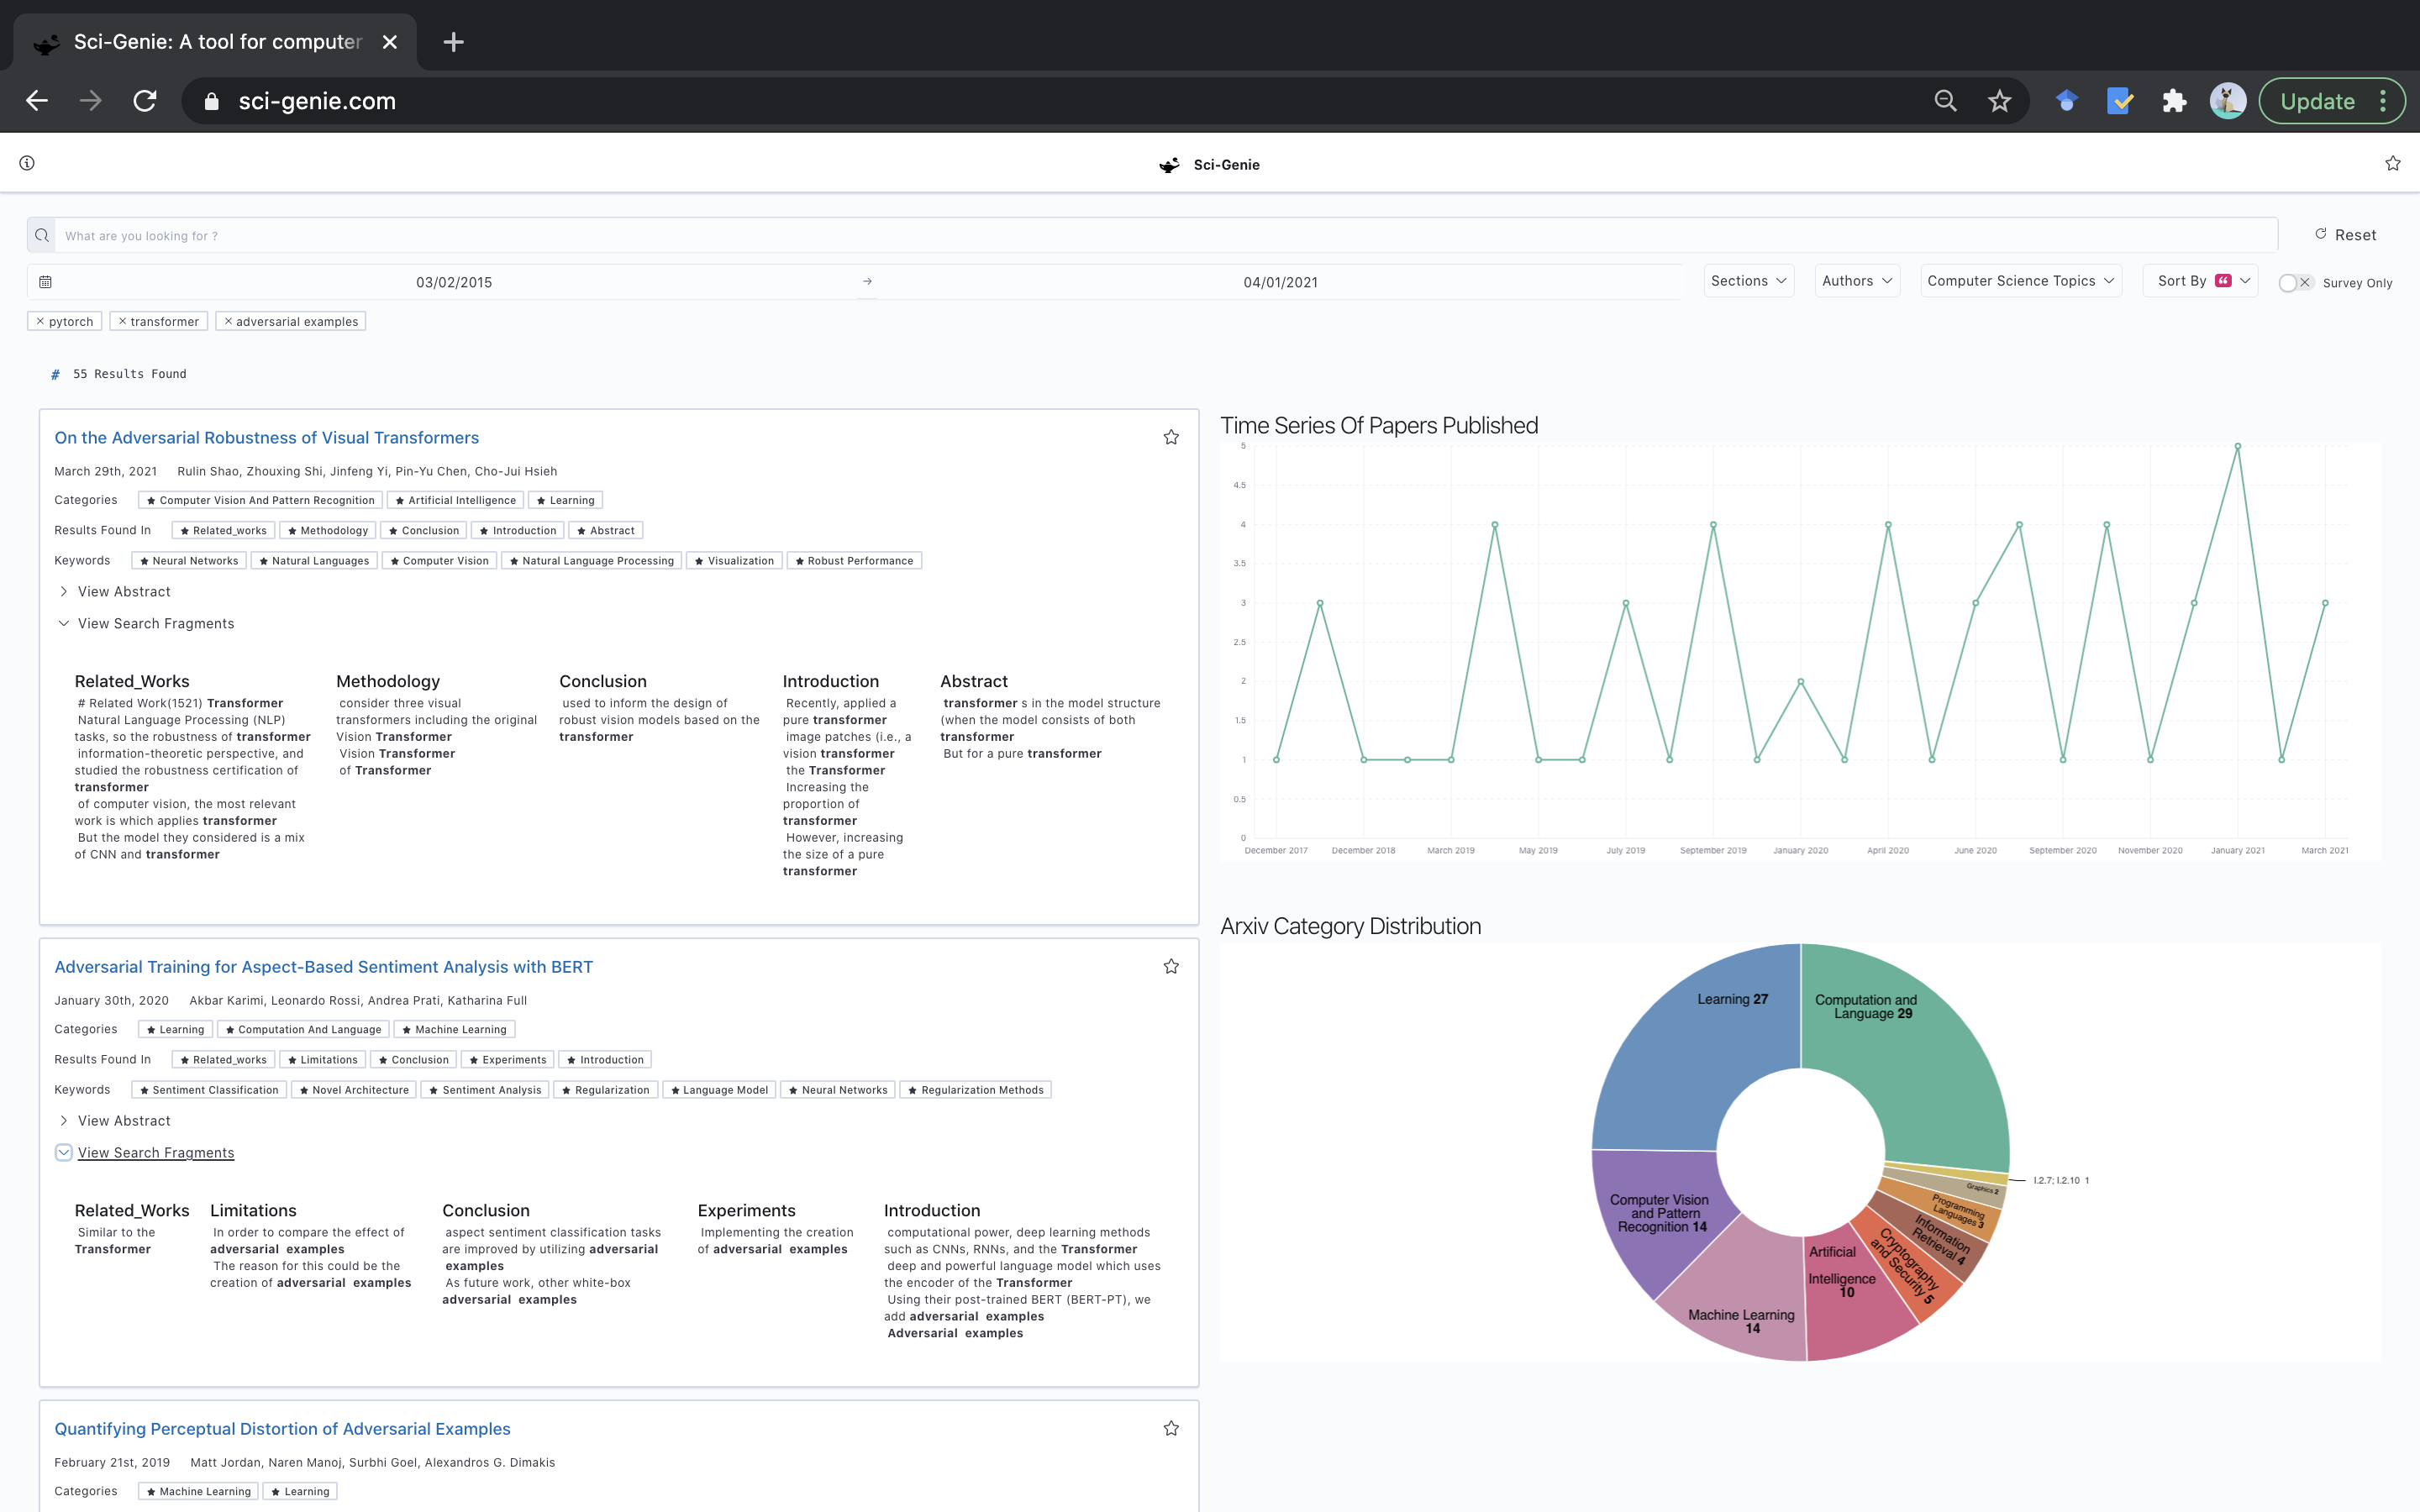
\includegraphics[width=\maxwidth{\textwidth}]{src/images/sci-genie-context-exp.png}
    \caption{Search Results With Context For Query \textit{pytorch, transformer, adversarial examples} Using Sci-Genie}
    \label{figure\arabic{figurecounter}}
\end{figure}
\refstepcounter{figurecounter}

Sci-Genie is a prototype search engine over CS ArXiv. 
Sci-Genie indexes the hierarchical structure of Computer Science research papers 
to provide more context to search results fragments. 
Sci-Genie's content mining engine also classifies a paper's ontology using a SOTA ontology classification model
developed by \cite{salatino2020ontology}. The mined ontology helps create a "Controlled Vocabulary" for filtering search results. 

\section{Sci-Genie-Extension: In-Browser Extension To Augment Information About Research }

\begin{figure}[h]
    \centering
    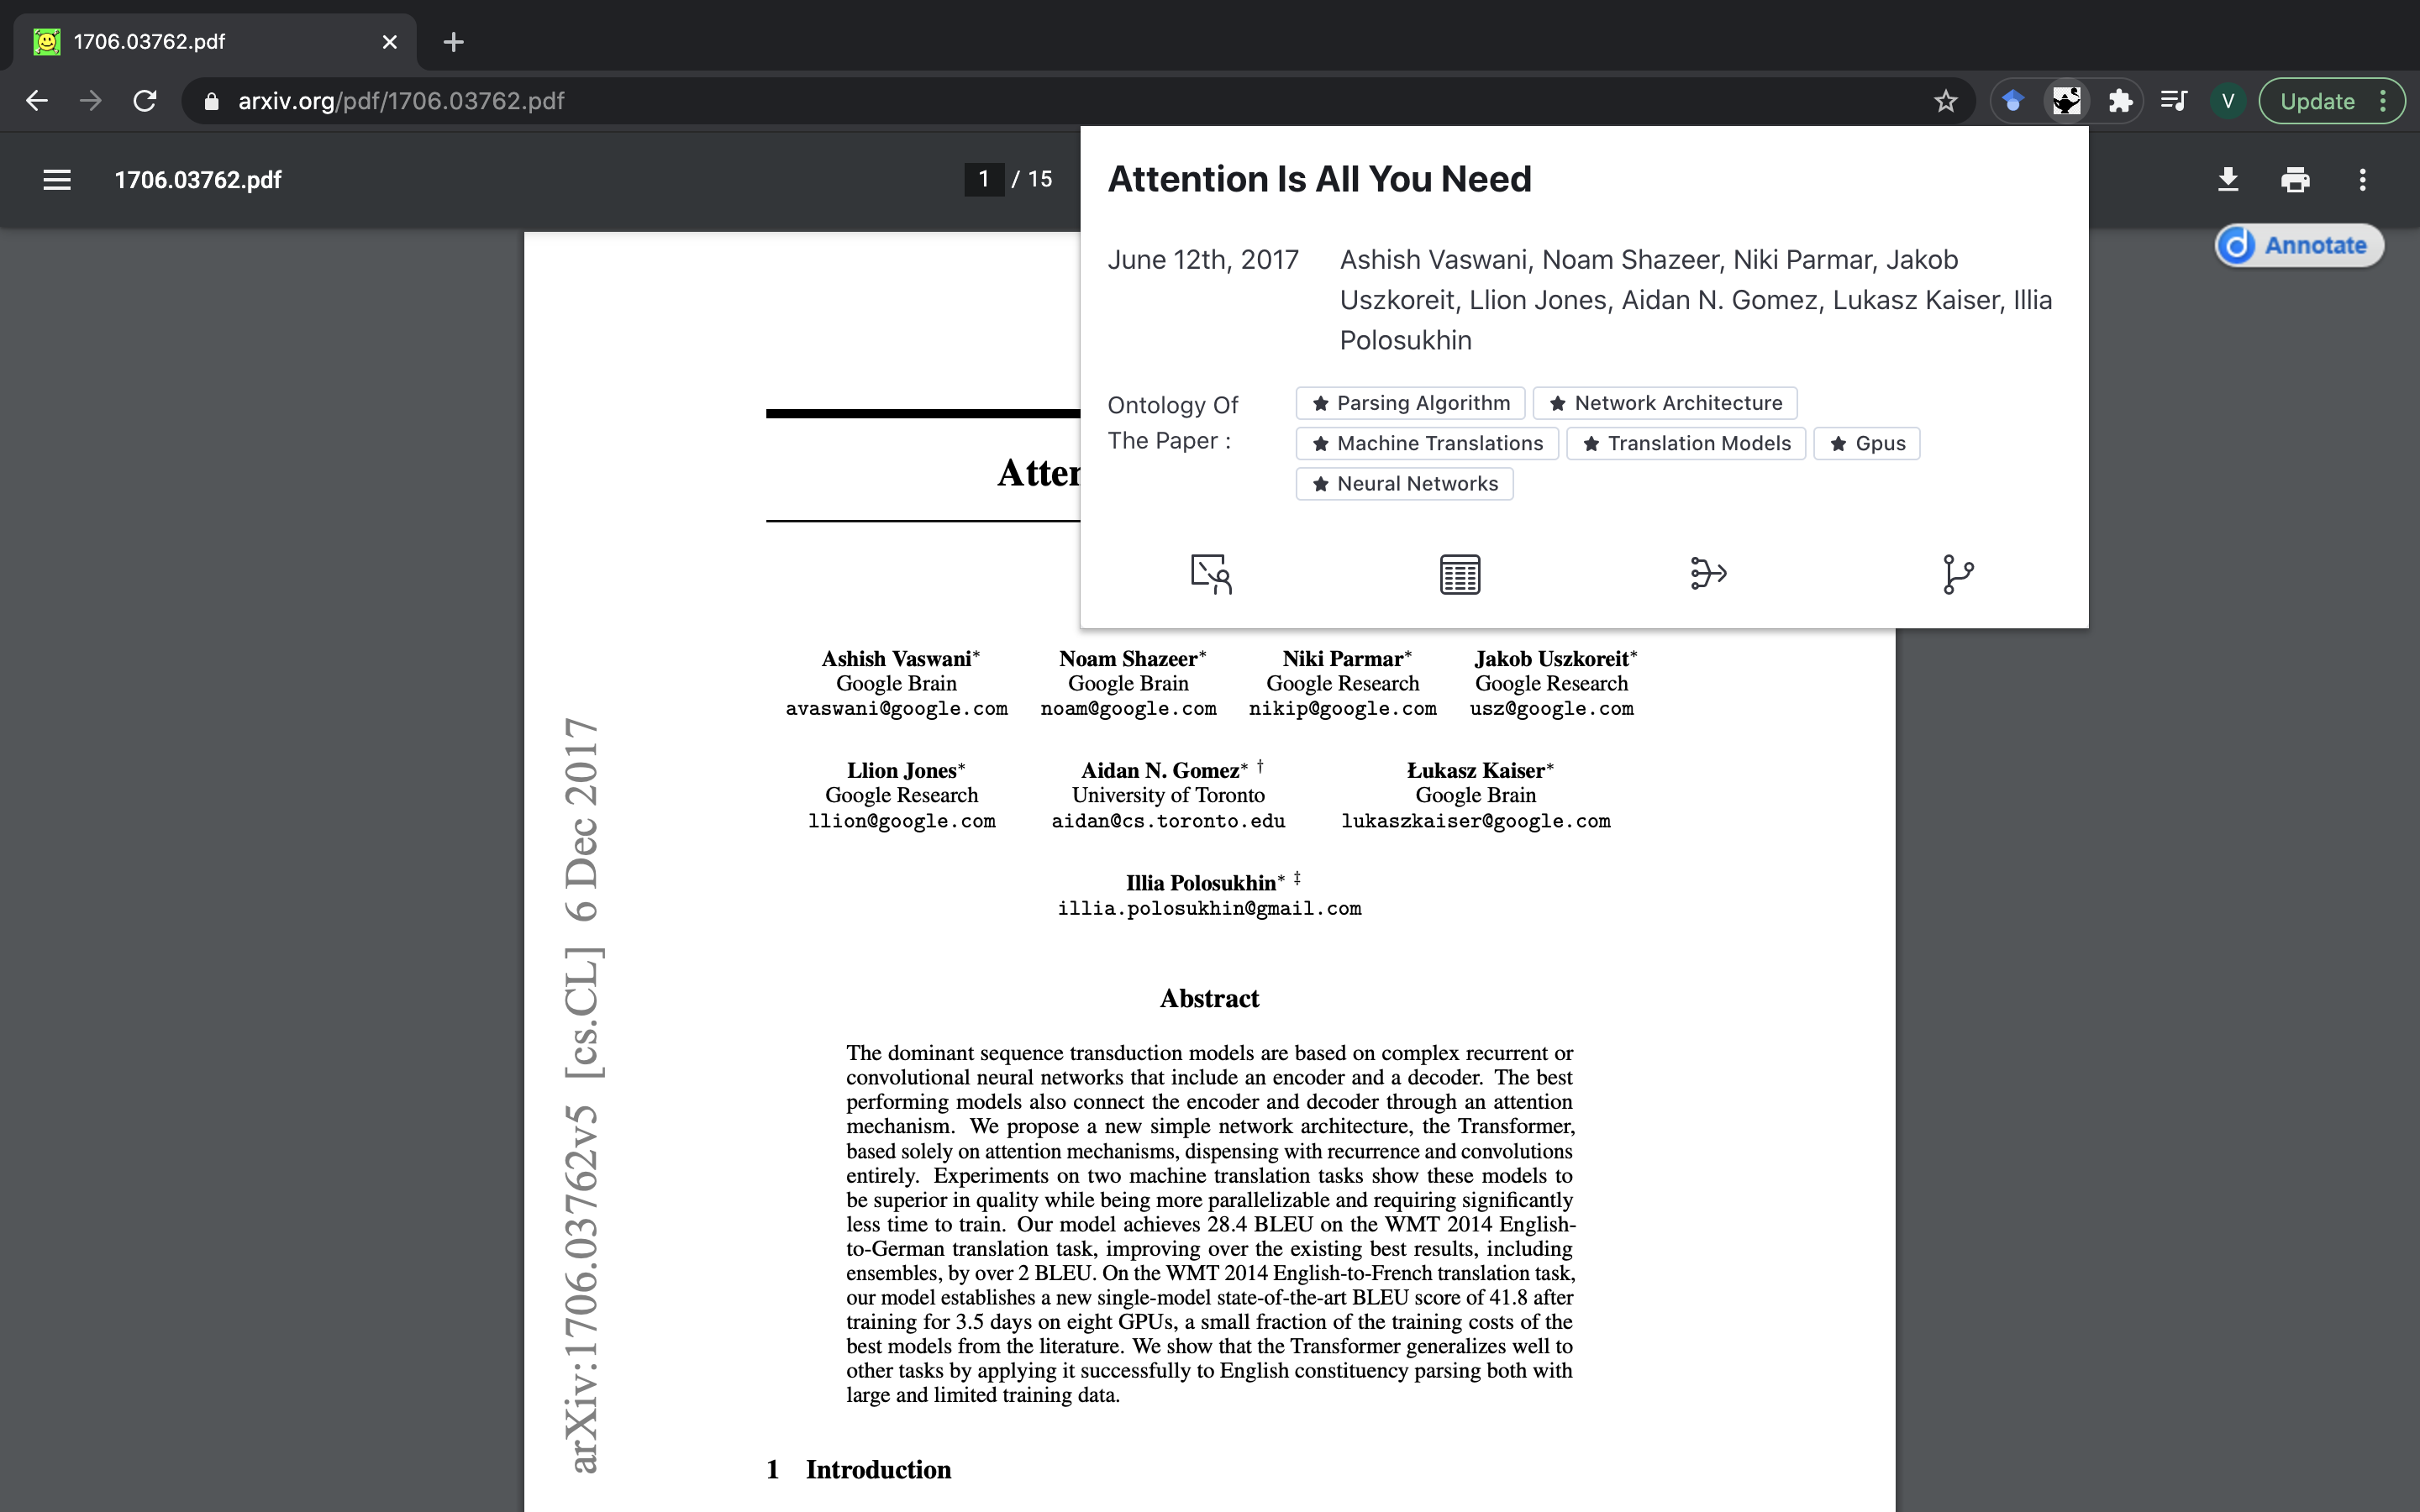
\includegraphics[width=\maxwidth{\textwidth}]{src/images/sci-genie-ext-exp.png}
    \caption{ Sci-Genie Browser Plugin}
    \label{figure\arabic{figurecounter}}
\end{figure}
\refstepcounter{figurecounter}

Sci-Genie, at its core, holds research from CS ArXiv, Tables from the paper mined from CS ArXiv and 
6.5M papers filtered from the Semantic Scholar Open Research Corpus\parencite{ammar-etal-2018-construction}.
The Semantic Scholar Open Research Corpus helps create a citation graph supporting information augmentation for the browser plugin. 

\begin{figure}[h]
    \centering
    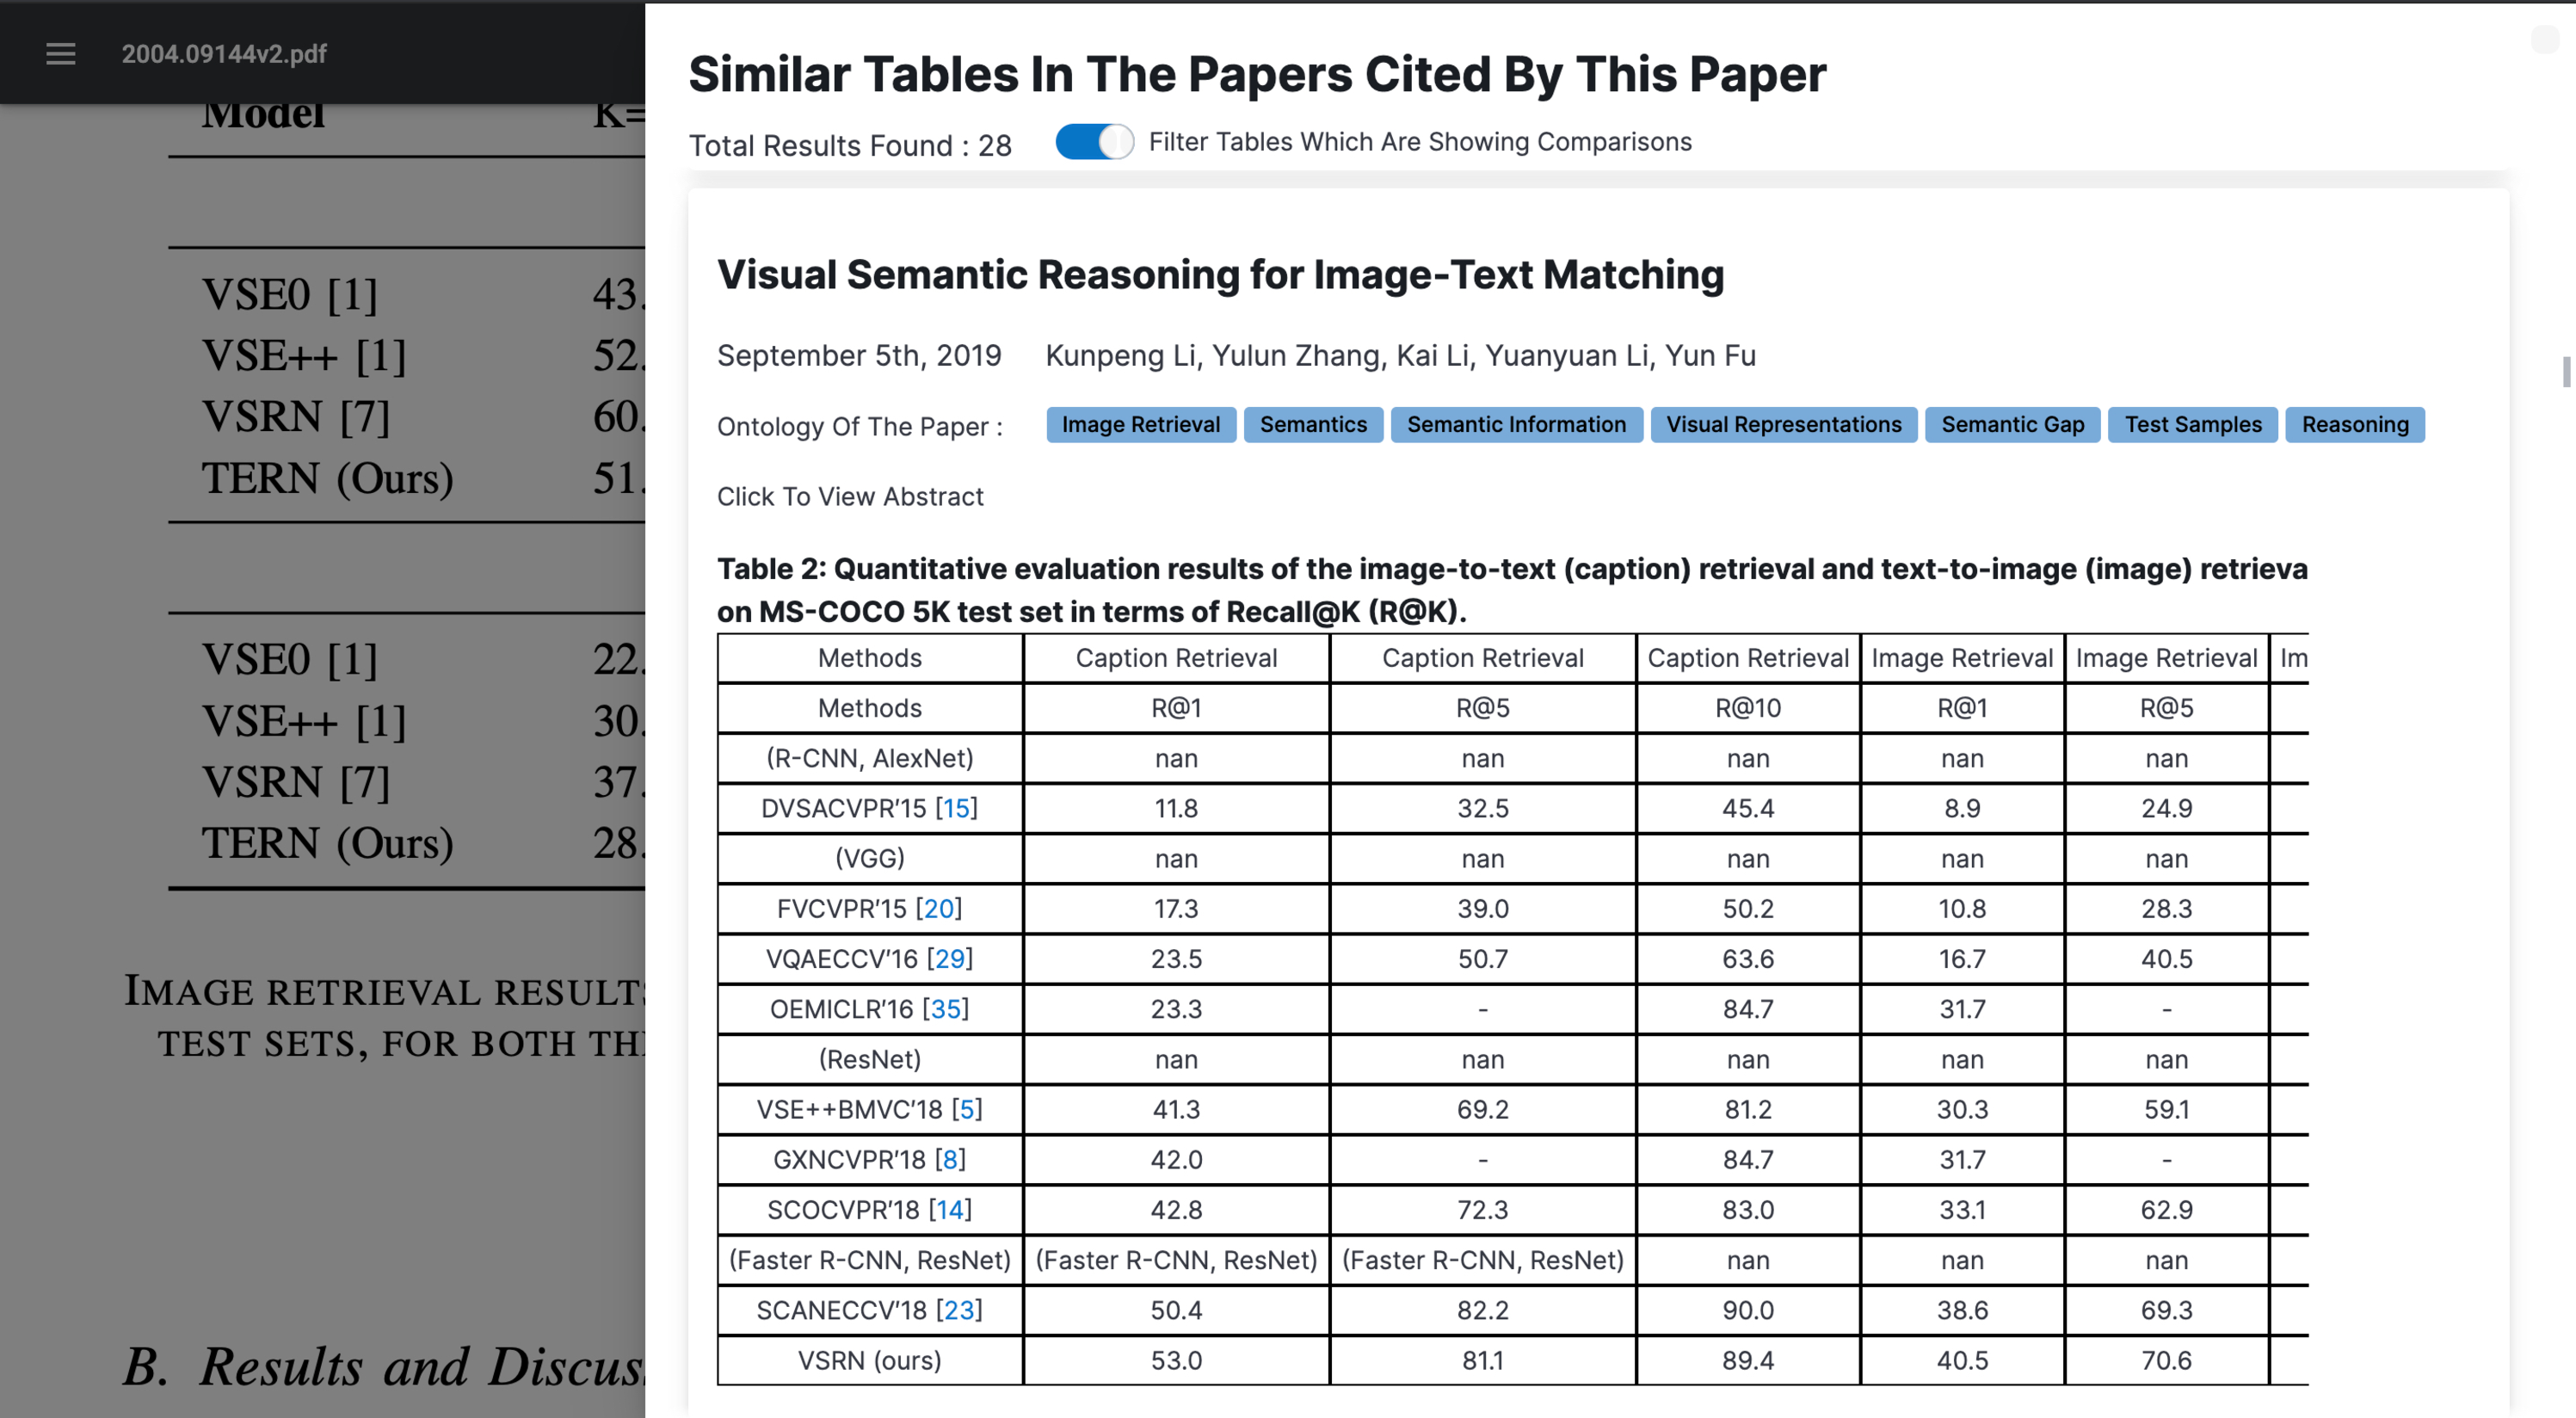
\includegraphics[width=\maxwidth{\textwidth}]{src/images/sci-genie-ext-table-comp-exp.pdf}
    \caption{Sci-Genie Browser Plugin surfacing information about tables comparing entities from cited papers.}
    \label{figure\arabic{figurecounter}}
\end{figure}
\refstepcounter{figurecounter}


\begin{figure}[h]
    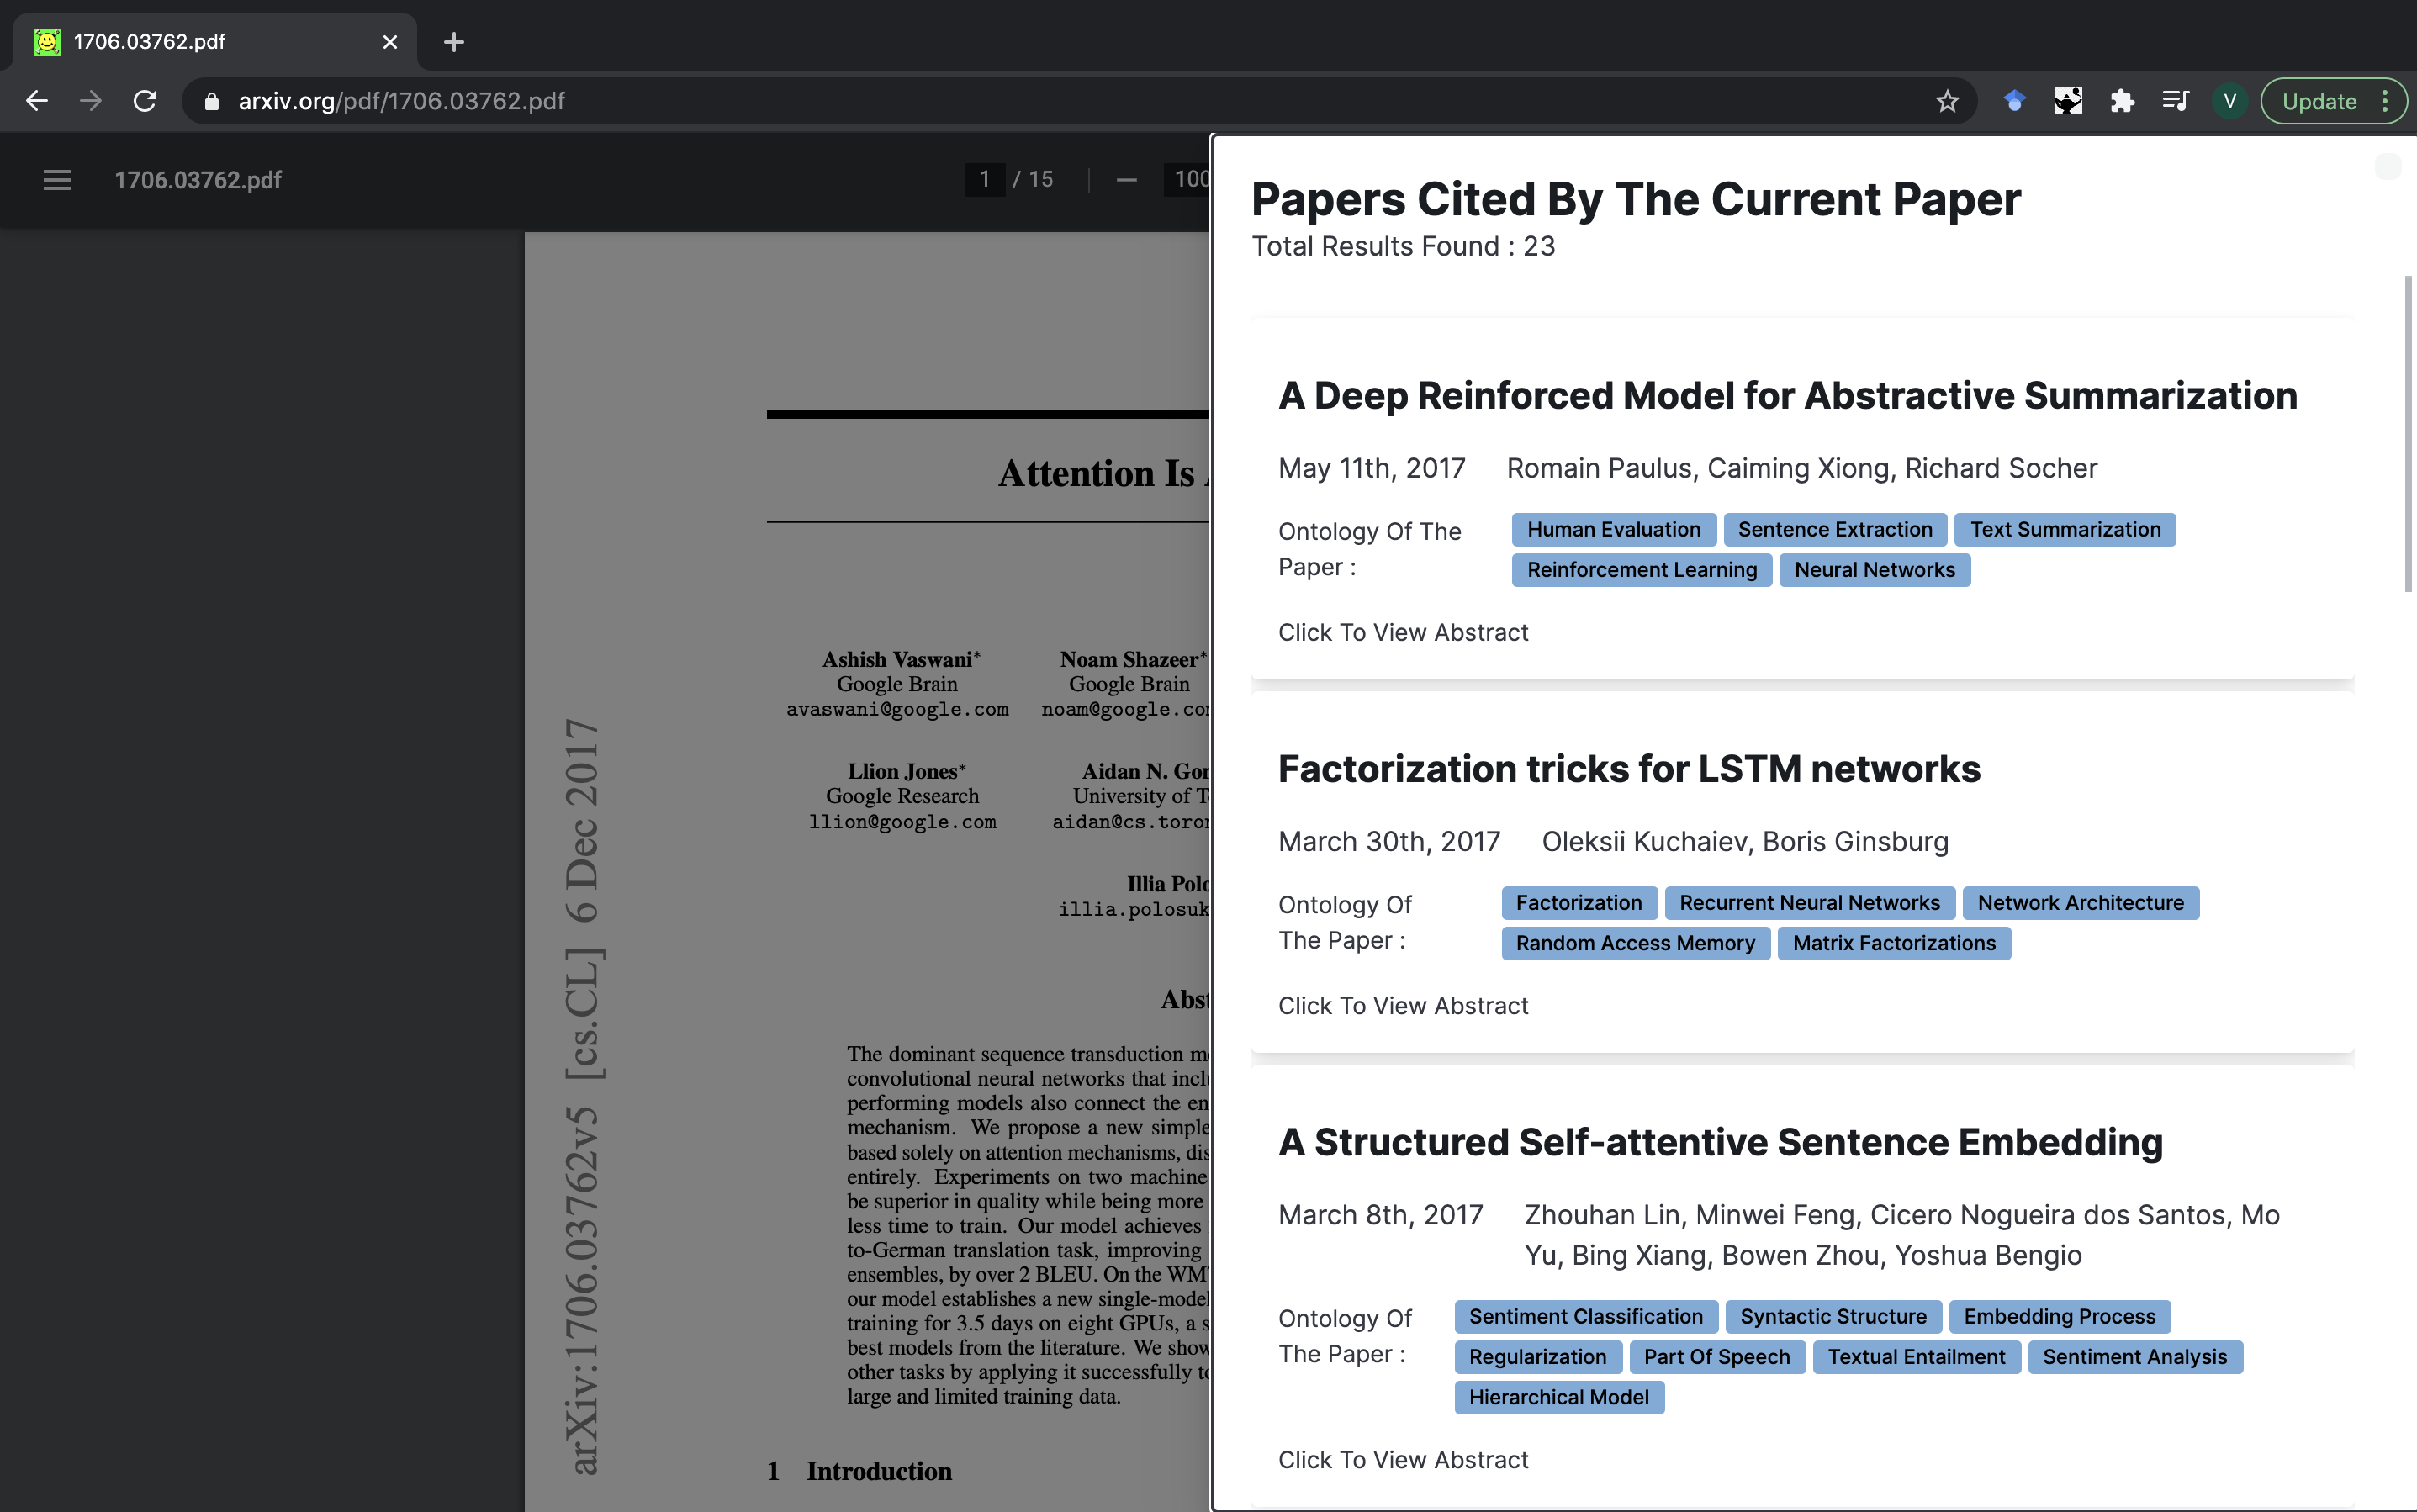
\includegraphics[width=0.475\textwidth]{src/images/sci-genie-ext-cite-out-exp.png}
    \hfill
    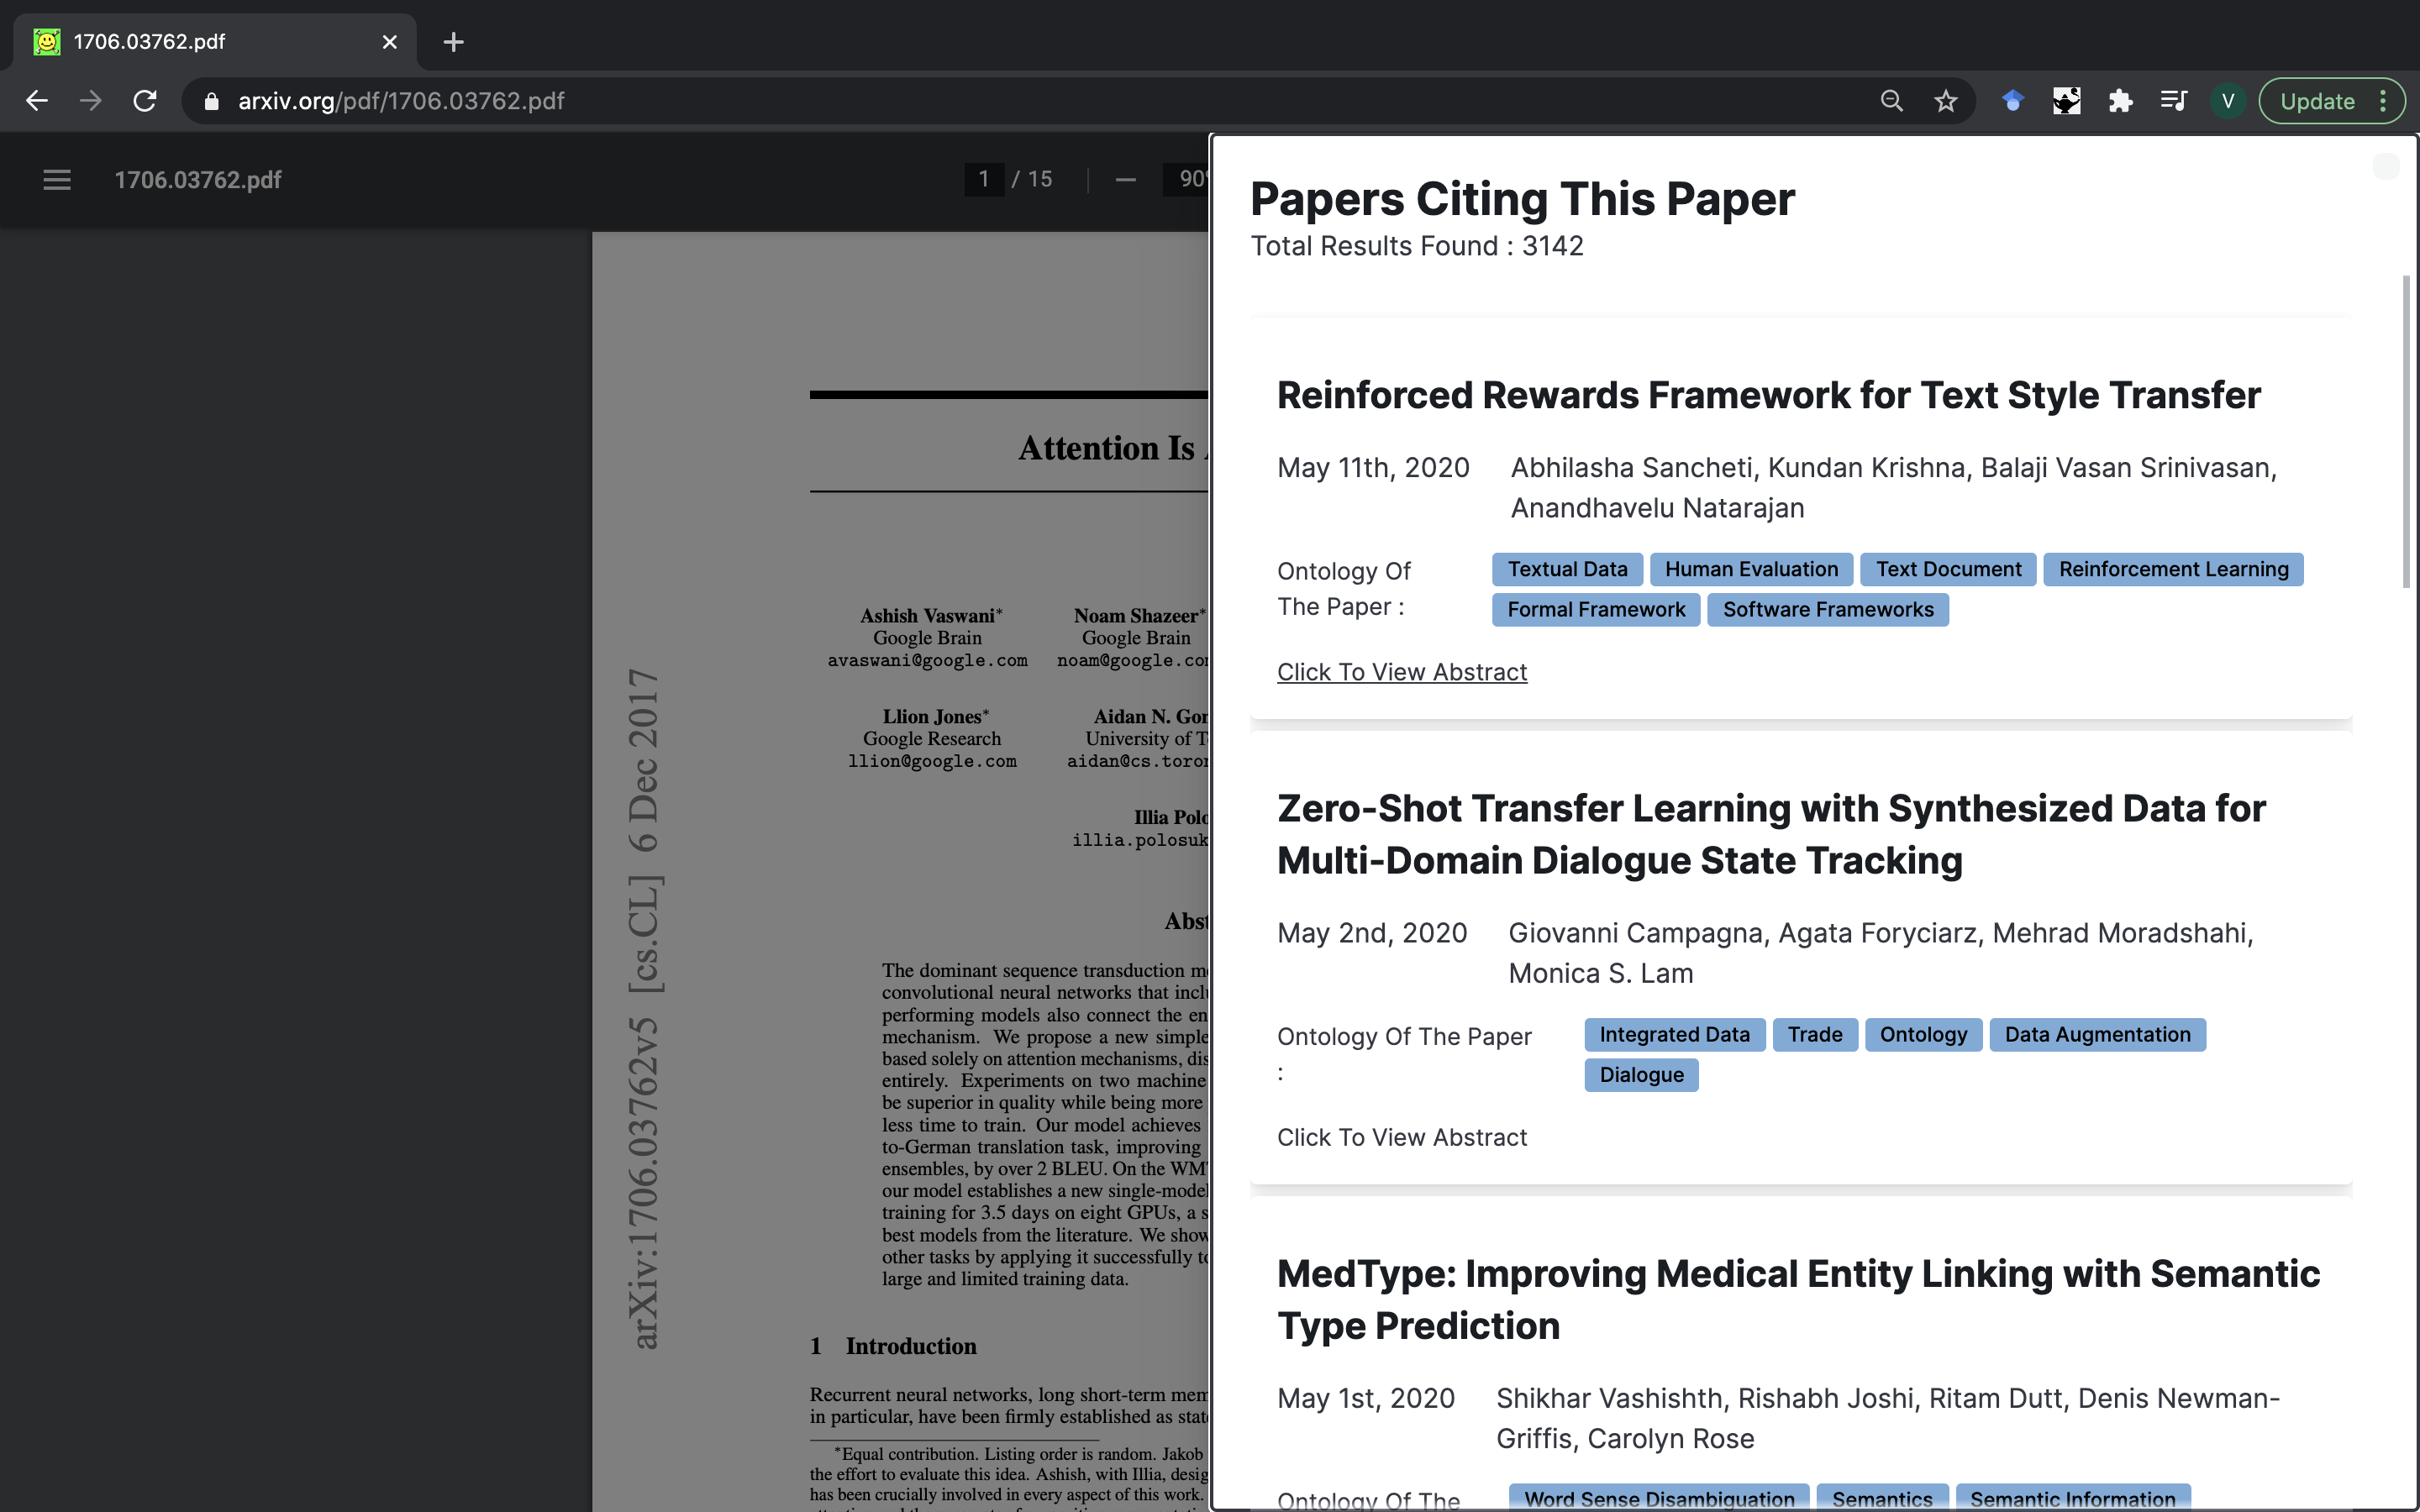
\includegraphics[width=0.475\textwidth]{src/images/sci-genie-ext-cite-exp.png}
    \caption{ Sci-Genie Browser Plugin surfacing context information about papers citing/cited-by the current paper }
    \label{figure\arabic{figurecounter}}
\end{figure}
\refstepcounter{figurecounter}

The citation graph helps surface context-relevant tables from papers cited by the paper the user is reading.  The search engine and the citation graph help extract other papers by the same authors and papers citing/cited by the paper the user reads. Figure \ref{figure10}, \ref{figure11},\ref{figure12}, shows an example of Sci-Genie extension in action. The browser extension also contains filters for filtering tables comparing entities using a machine learning model. All information provided by the browser extension helps enhance the researcher’s understanding without the researcher having to dig up the information independently. 

\begin{figure}[h]
    \centering
    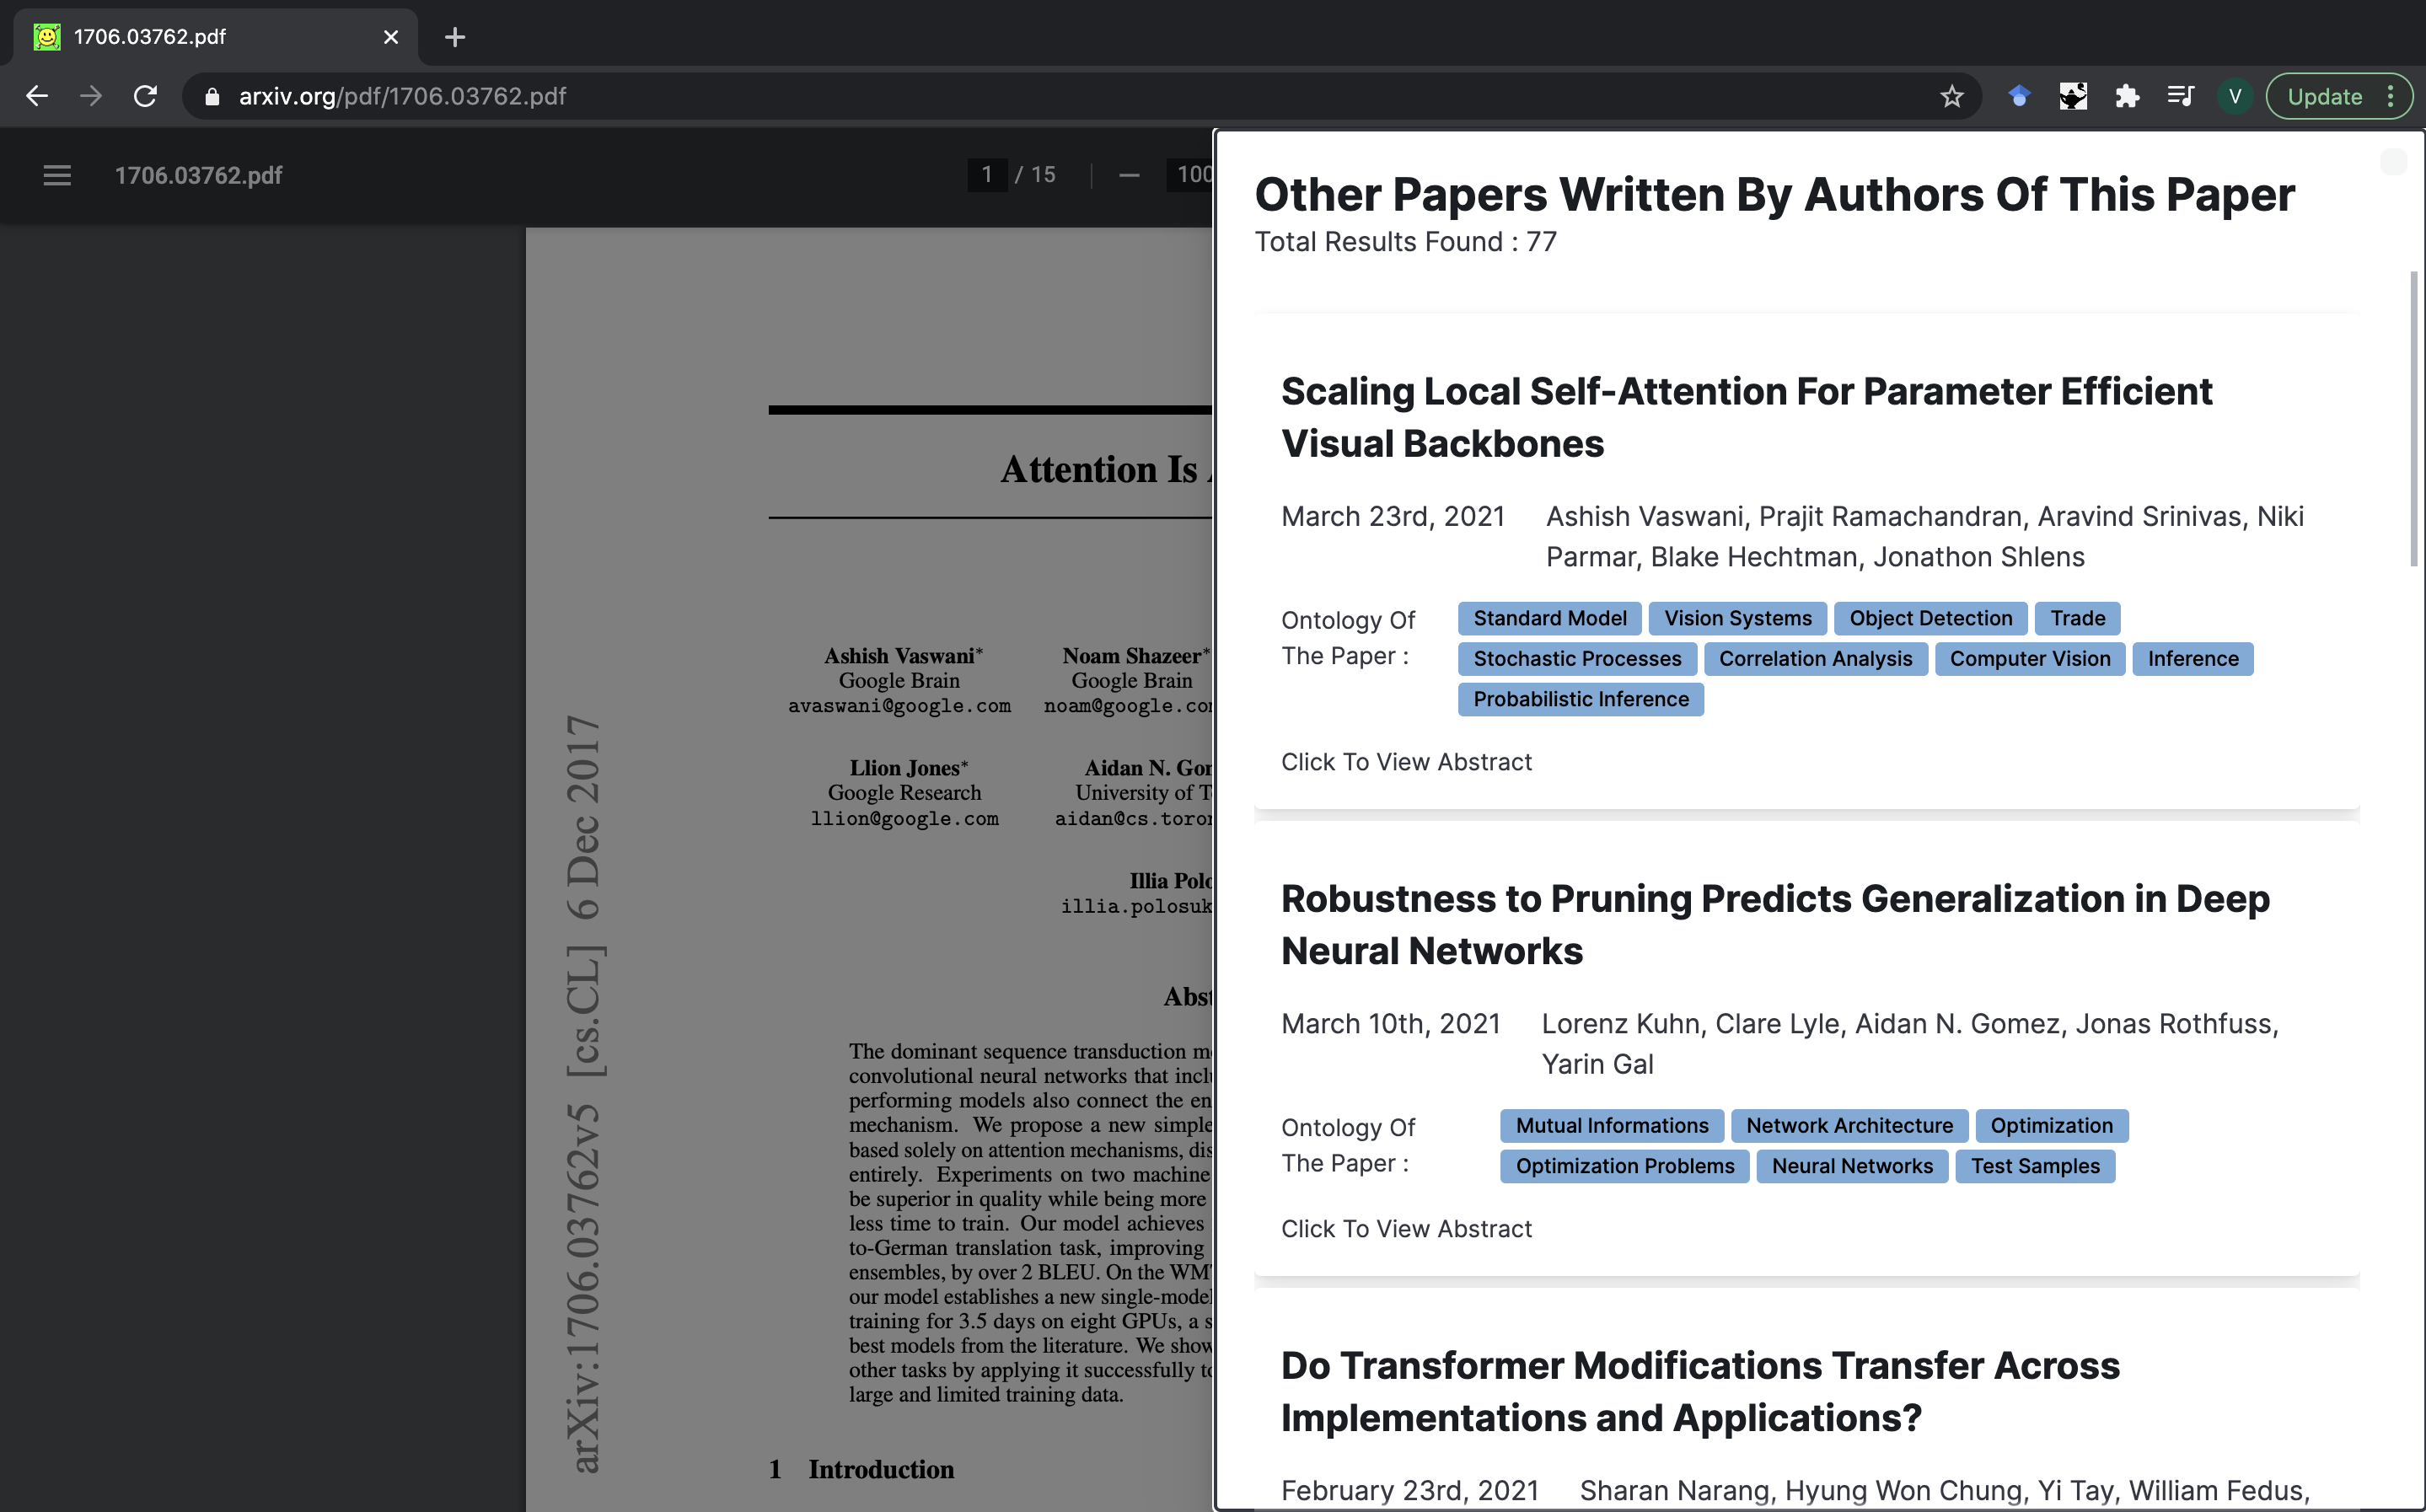
\includegraphics[width=\maxwidth{\textwidth}]{src/images/sci-genie-ext-authors-exp.png}
    \caption{ Sci-Genie Browser Plugin surfacing information about other papers from the authors of the paper the user is reading}
    \label{figure\arabic{figurecounter}}
\end{figure}
\refstepcounter{figurecounter}

\subsection{Design Choices}
Sci-Genie uses ArXiv as a source for papers because ArXiv provides the availability of LaTeX sources. LaTeX based sources are easier to parse compared to PDF documents because of LaTeX's compilability. As LaTeX is Turing complete, the compiled content’s parse tree is easily accessible compared to PDFs. Due to this, Sci-Genie doesn't parse PDF documents. 
\chapter{Sci-Genie Core}
\label{sci-genie-core}
\begin{figure}[p]
    \centering
    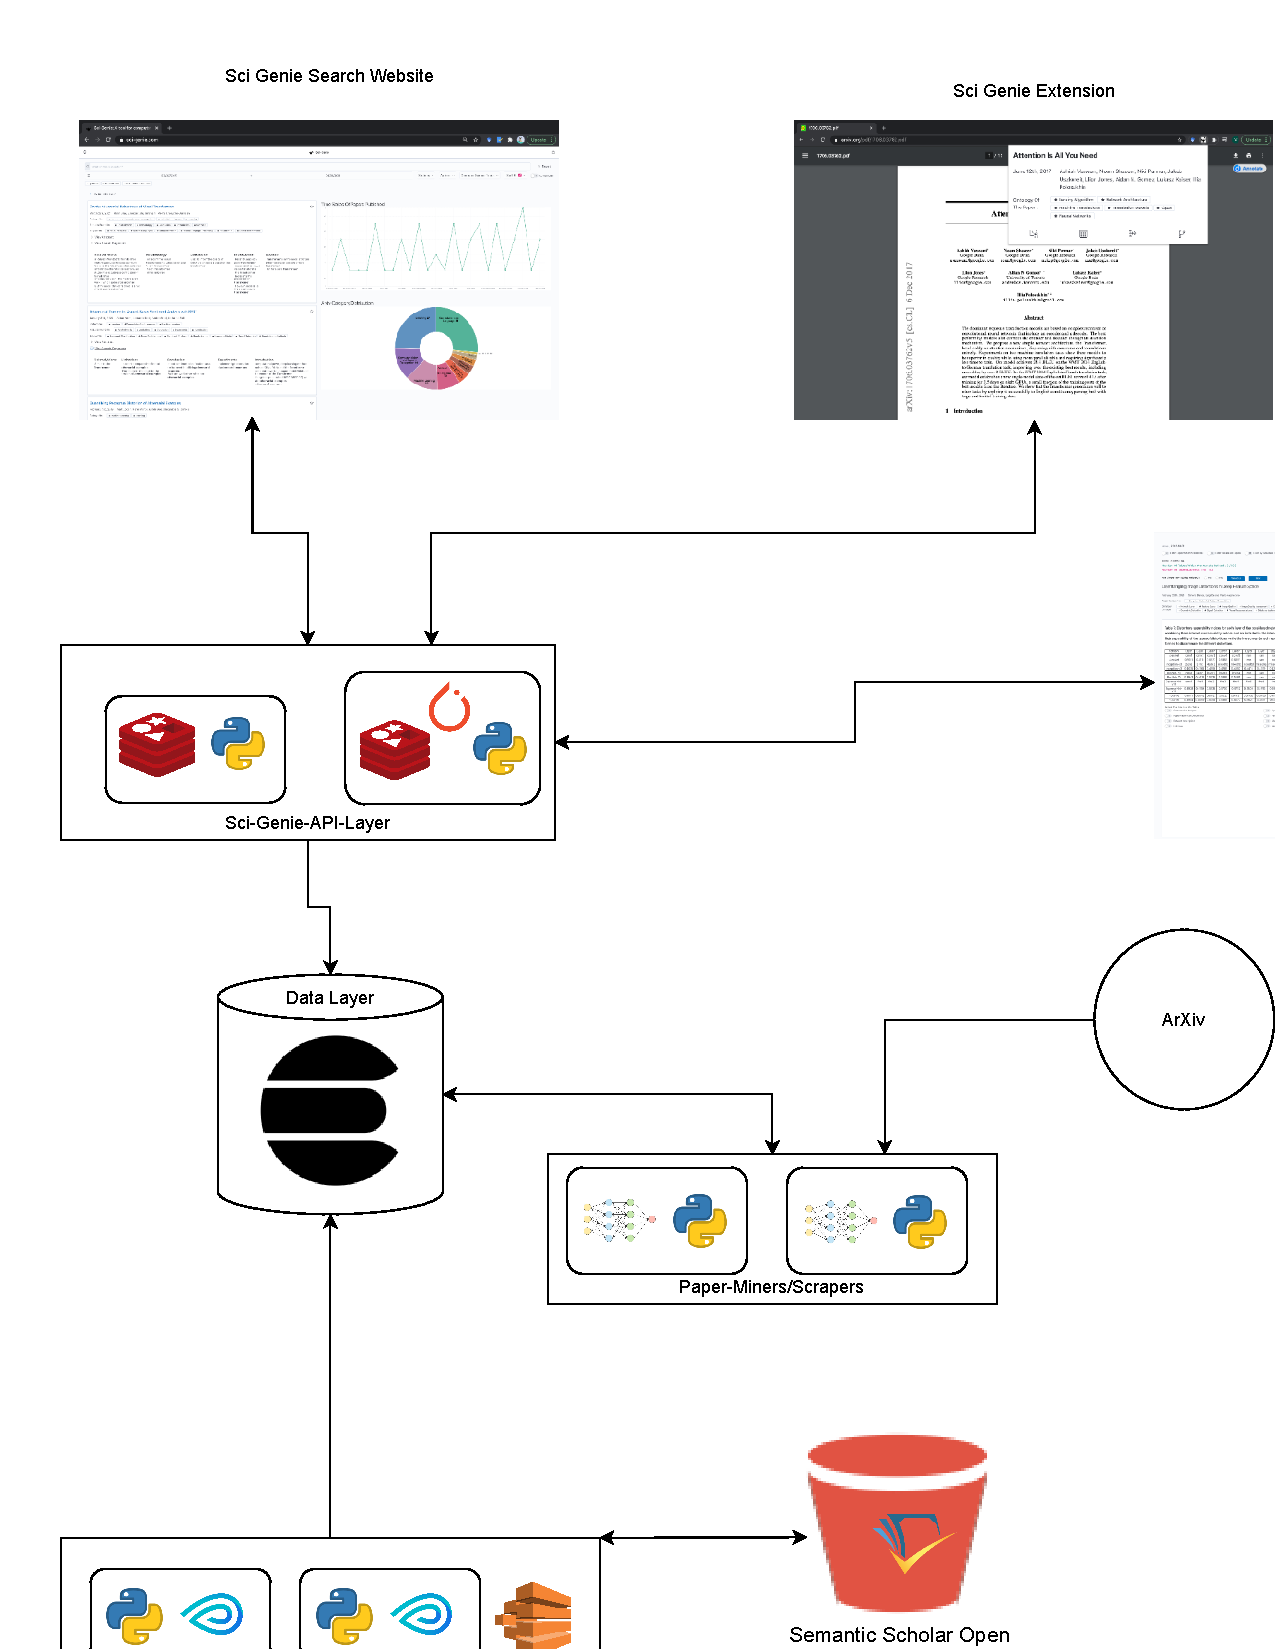
\includegraphics[width=\maxwidth{\textwidth}]{src/images/Sci-Genie-Arch.pdf}
    \caption{Sci-Genie System Architecture}
    \label{figure\arabic{figurecounter}}
\end{figure}
\refstepcounter{figurecounter}
% \pagebreak

\section{System Architecture}

Sci-Genie Core comprises four key architectural components which help power information for multiple different apps like the browser-extension, the website and the labeling interfaces for machine learning. 
\begin{itemize}
    \item \textbf{Data Layer}
    \item \textbf{API Layer}
    \item \textbf{Paper Scraping And Mining Engine}
    \item \textbf{Semantic Scholar Citation Graph Mining Engine}
\end{itemize}

Paper Scraping And Mining Engine help extract papers From ArXiv in LaTeX format and then parses the structure, mines the ontology, and extracts the tables. The processed information gets stored in the Data Layer. 

The Data Layer hosts the information used by the website or the browser extension. 

The Semantic Scholar Citation Graph Mining Engine leverages a data processing pipeline to filter CS research and create an index in the Data Layer, containing information corresponding to citations of papers from ArXiv. 

The API Layer leverage the general-purpose abstractions built around the Data Layer to access and further intelligently process information at search time. The API Layer connects the Data Layer with various applications like The Sci-Genie Website, The Sci-Genie extension and other apps such as the Table Labeling tool. 

\section{Sci-Genie Data Layer}
\label{sci-genie-core:data-layer}
The Data Layer comprises the open-source search engine named Elasticsearch\parencite{gormley2015elasticsearch} which is built on top of Lucene. 
The data layer aims to host processed information after scraping, mining, and parsing research documents and tables. 
Elasticsearch hosts the following indexes\footnote{Index is similar to Database in the language of RDBMS}\footnote{https://www.elastic.co/guide/en/elasticsearch/reference/current/documents-indices.html} to filter access of content:
\begin{itemize}
    \item \textbf{Arxiv Parsed Research Index}:\textit{Contains research documents whose structure is explicitly parsed and stored}
    \item \textbf{Semantic Scholar Index}:\textit{Contains documents from the CS Domains mined and filtered from semantic scholar open research corpus}
    \item \textbf{Arxiv Table Index}:\textit{Stored the tables from research papers which can be later used for information augmentation.}
    \item \textbf{Arxiv Semantic Scholar Join Index}:\textit{Stores the citation information filtered from semantic scholar index to map papers in ArXiv} 
\end{itemize} 

\subsection{Arxiv Parsed Research Index}

Documents in the Arxiv Parsed Research Index helps power the search for the Sci-Genie search website. All documents belong to Computer Science ArXiv and 
the construction of these documents is discussed in Section \ref{sci-genie-core:scraping}. Each document consists of three 
key pieces of information:
\begin{itemize}
    \item \textbf{ArxivIdentity} \textit{ArXiv associated meta-data information}
    \item \textbf{ResearchObject} \textit{Parsed Research structure}
    \item \textbf{Ontology} \textit{Ontology belonging to the article.}
\end{itemize}

\subsubsection{ArxivIdentity}
ArXiv associated meta-data information holds information regarding the abstract, title, authors, categories of the paper etc. 
The information stored in this object helps provide search stratagems to the Sci-Genie search website. 

\subsubsection{ResearchObject}
\label{sci-genie-core:data-layer:researchobj}
The ResearchObject is the data structure that holds the parsed text from the research document. 
The purpose of this object is to fit the research document and its hierarchy into predefined sections
which are commonly occurring in research documents. The general pre-identified sections are given below:
\begin{itemize}
    \item Introduction
    \item Related Works
    \item Methodology
    \item Experiments
    \item Dataset
    \item Conclusion
    \item Limitations
\end{itemize} 
Any section that doesn't fit the predefined sections will be categorized as \textit{Unknown}. 

The ResearchObject consists of key value pairs which relate to the given predefined sections. The key is the name of the section eg. Introduction, Related Works etc. and the value is a \textit{Fragment}. 
Fragment is a tree-like data structure that holds hierarchical information. Fragment is given by:
\begin{verbatim}
    class Fragment:
        title:str = "Introduction"
        text:str = "Text relating to the introduction of a paper"
        children:List[Fragment] 
\end{verbatim}    

The \textit{children} in the Fragment hold the information about the child notes of that Fragment. The Fragment object helps capture a research paper’s hierarchy before it gets parsed into a key-value-based ResearchObject. The Fragment object can also be serialized to JSON making it indexable in the Lucene search index.  

Due to the search engine’s scope being limited to CS research on ArXiv, the predefined sections are created based on a statistical analysis of the content after scraping. Section \ref{sci-genie-core:scraping} provides more details on the creation of the Fragment and ResearchObject. 

\paragraph{Advantages Of Indexing ResearchObject}
The ResearchObject is a key value-based object, and each key allows indexing the text according to its corresponding section. This object schema helps provide more context about the search match within each section, as seen from Figure \ref{figure7}. 

\subsubsection{Ontology}
\begin{figure}[h]
    \centering
    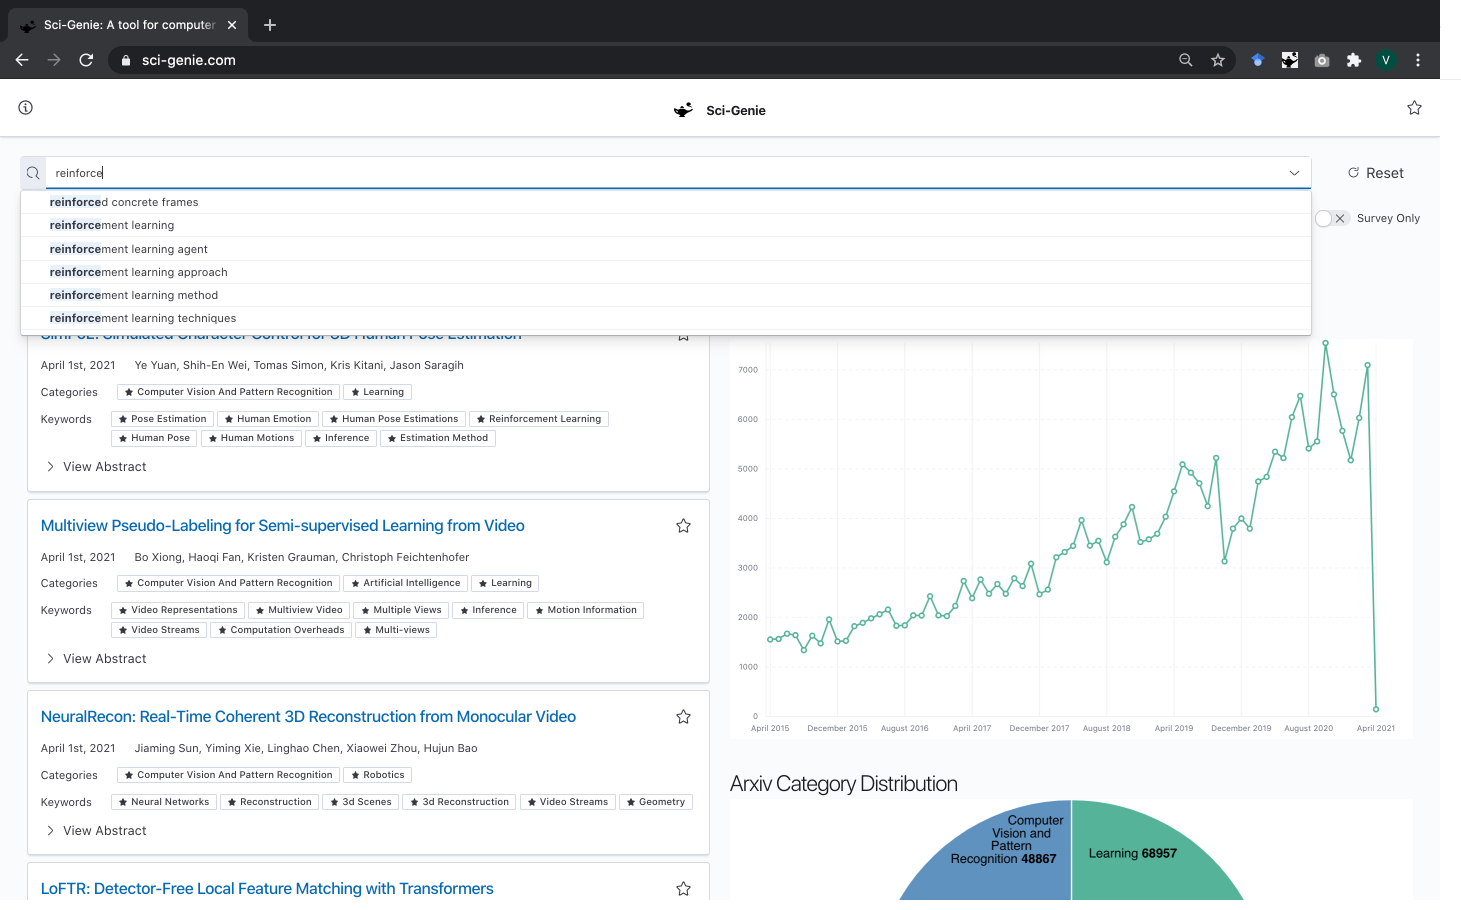
\includegraphics[width=\maxwidth{\textwidth}]{src/images/sci-genie-autocomp-example.png}
    \caption{Sci-Genie auto-completing the search terms using the ontology}
    \label{figure\arabic{figurecounter}}
\end{figure}
\refstepcounter{figurecounter}

The study conducted by \cite{li2017investigating} gave a great indicator regarding the need for entity based queries in academic research search engines to improve precision. As Sci-Genie only operates over computer science research, the research papers’ ontology helps power the autocomplete panel in the search bar from Figure \ref{figure13}. Each paper consists of an ontology which is classified via CS specific ontology classifier.\footnote{https://github.com/angelosalatino/cso-classifier\#sample-output-sp}. Sci-Genie indexes the entire ontology given by \cite{salatino2020ontology}. 

\subsection{Semantic Scholar Index}
\label{sci-genie-core:data-layer:ss-index}
This index hosts information filtered from the Semantic Scholar Open Research Corpus\parencite{ammar-etal-2018-construction} post Citation Graph Mining. More details on how it is filtered is described in Section \ref{sci-genie-core:citation-mining}. This index’s core purpose is to help correlate citation to and from papers on ArXiv. The Sci-Genie extension further uses this citation information for finding tables from the neighborhood of papers as seen in Figure \ref{figure9}. 


\subsection{Arxiv Table Index}
\label{sci-genie-core:data-layer:table-index}
This index holds information regarding the tables from a research paper. The core methodology which is used to extract and serialize/deserialize tables from LateX is based the methodology developed by \cite{kardas2020axcell}. The method created by  \cite{kardas2020axcell} helps convert tables in pandas\footnote{https://pandas.pydata.org/} serializable DataFrames. These DataFrames can be serialized to json for storage in Elasticsearch. The schema for the object can seen below : 
\begin{verbatim}
    class ArxivTable:
        semantic_scholar_id:str = ""
        arxiv_id:str=""
        identity:str = ""
        figure_id:str=""
        caption:str=""
        name:str=""
        layout:str=""
        table:str=""
\end{verbatim}

The \textit{identity} is the unique identifier for a table. Each record also holds loose relations to the Arxiv Parsed Research Index and the Semantic Scholar Index via respective ids. 

\subsection{Arxiv Semantic Scholar Join Index}
\label{sci-genie-core:data-layer:ss-join-index}
This index holds references of in and out citations for each ArXiv article present in the Arxiv Parsed Research Index. Although the Semantic Scholar Index contains citation data, none of it is correlated with ArXiv articles and hence this index is created to help correlate information at search time. Below is the schema for the documents in the index: 
\begin{verbatim}
    {
        "in_citn_arxiv": [],
        "out_citn_arxiv": [],
        "semantic_scholar_id": "",
        "arxiv_id": "",
}
\end{verbatim}
The \textit{arxiv\_id} is the unique ArXiv identifier, The \textit{in\_citn\_arxiv} correspond to the unique ArXiv ids of papers that cited a paper. The \textit{out\_citn\_arxiv} correspond to the unique ArXiv ids of papers cited by a paper. This information comes of great use when filtering out tables as seen in Figure \ref{figure9}. The construction of this index is discussed in Section \ref{sci-genie-core:citation-mining}
% The ontology of research papers is stored in the same form as provided by the 
\section{Paper Scraping And Mining Engine}
\label{sci-genie-core:scraping}
The Paper Scraping And Mining Engine connects with ArXiv to extract LaTeX source data. The LaTeX source data undergoes three parallel processing steps:
\begin{itemize}
    \item Content Hierarchy Parsing : The extraction of content based on document structure for storage
    \item Ontology Mining : Correlating the ontology of the paper from ArXiv
    \item Table Extraction : Leveraging tools to extract tables from the ArXiv document's LaTeX source.
\end{itemize}

\subsection{Content Hierarchy Parsing}
A structured \nameref{sci-genie-core:data-layer:researchobj} is parsed from raw LateX content in two steps:
\begin{itemize}
    \item Step 1 : Extract the structure of the research document and create a Fragment object
    \item Step 2 : Correlate the children in the Fragment Object with predefined sections to create the \nameref{sci-genie-core:data-layer:researchobj} 
\end{itemize} 
\subsubsection{Fragment Creation}
\label{sci-genie-core:scraping:source-frag}
Each LaTeX source repository is parsed to create a "Structure Tree" of the research document. The Structure tree\footnote{https://github.com/alvinwan/tex2py} helps correlate the structure of latex document. The structure tree is then used to create Fragment objects described in Section \ref{sci-genie-core:data-layer:researchobj}. The text within each Fragment is populated by using the opendetex library\footnote{https://github.com/pkubowicz/opendetex}. The opendex library helps filter text information from individual tex files. The code to match the structure tree is provided in the Appendix. 

\subsubsection{ResearchObject Creation From Fragment}
\label{sci-genie-core:scraping:frag-to-rs}
The initial Fragment object created via the parsing described earlier will contain the entire research document stored in a single Fragment. This Fragment then undergoes a "heuristic" serialization to the ResearchObject. Meaning the title of the children within the Fragment is matched to predefined sections/classes given in Section \ref{sci-genie-core:data-layer:researchobj}. The matching process uses heuristics to match the content. More details on the section name matching strings and algorithm are given in the Appendix \ref{appendix:content-parsing-code} and \ref{appendix:mapping-heuristic} respectively. 

\subsection{Ontology Mining}
Sci-Genie leverages the ontology mining method described by the \cite{salatino2020ontology}. The research document's abstract and title are only needed for ontology mining. 

\subsection{Table Extraction and Storage}
To extract tables from papers on ArXiv, Sci-Genie uses arxiv-vanity/engrafo\footnote{https://github.com/arxiv-vanity/engrafo} to convert LaTeX to HTML and then employ table serialization methods created by \cite{kardas2020axcell}. The parsed tables are stored in the \nameref{sci-genie-core:data-layer:table-index}. 


\section{Semantic Scholar Citation Graph Mining.}
\label{sci-genie-core:citation-mining}
A rich source of context and metadata about the tables cited by a paper comes via the access to citations in a paper and leveraging the citation graph. The Semantic Scholar\footnote{http://s2-public-api-prod.us-west-2.elasticbeanstalk.com/corpus/} corpus consists of 136M research papers from various domains with their citations. This corpus event consists of all urls to a research paper, including the ones on ArXiv.  

Metaflow\footnote{https://metaflow.org/} is used to create a data processing pipeline\footnote{https://github.com/valayDave/semantic-scholar-data-pipeline} for filtering the subset of CS papers from the Semantic Scholar corpus. The filtered CS papers are stored in the \nameref{sci-genie-core:data-layer:ss-index}. 

The pipeline further correlates the citations of papers which are present on ArXiv and stores them in the \nameref{sci-genie-core:data-layer:ss-join-index}. 
% The Semani .

\section{API Layer}
The API layer is Sci-Genie, which leverages the general-purpose abstractions built over the DataLayer to access and process information for various apps such as the search engine website, the chrome plugin and the table labeling interface. 

\subsection{Scientific Table Correlation Via Citation Graphs}
With the access to distinctly processed and correlated information about research papers on ArXiv and their associated tables, the API Layer leverages these traits to filter tables from papers that cited the paper the user is reading (as seen in Figure \ref{figure14} and \ref{figure9}). 


\subsection{Table Of Comparison Classification}
\begin{figure}[h]
    \centering
    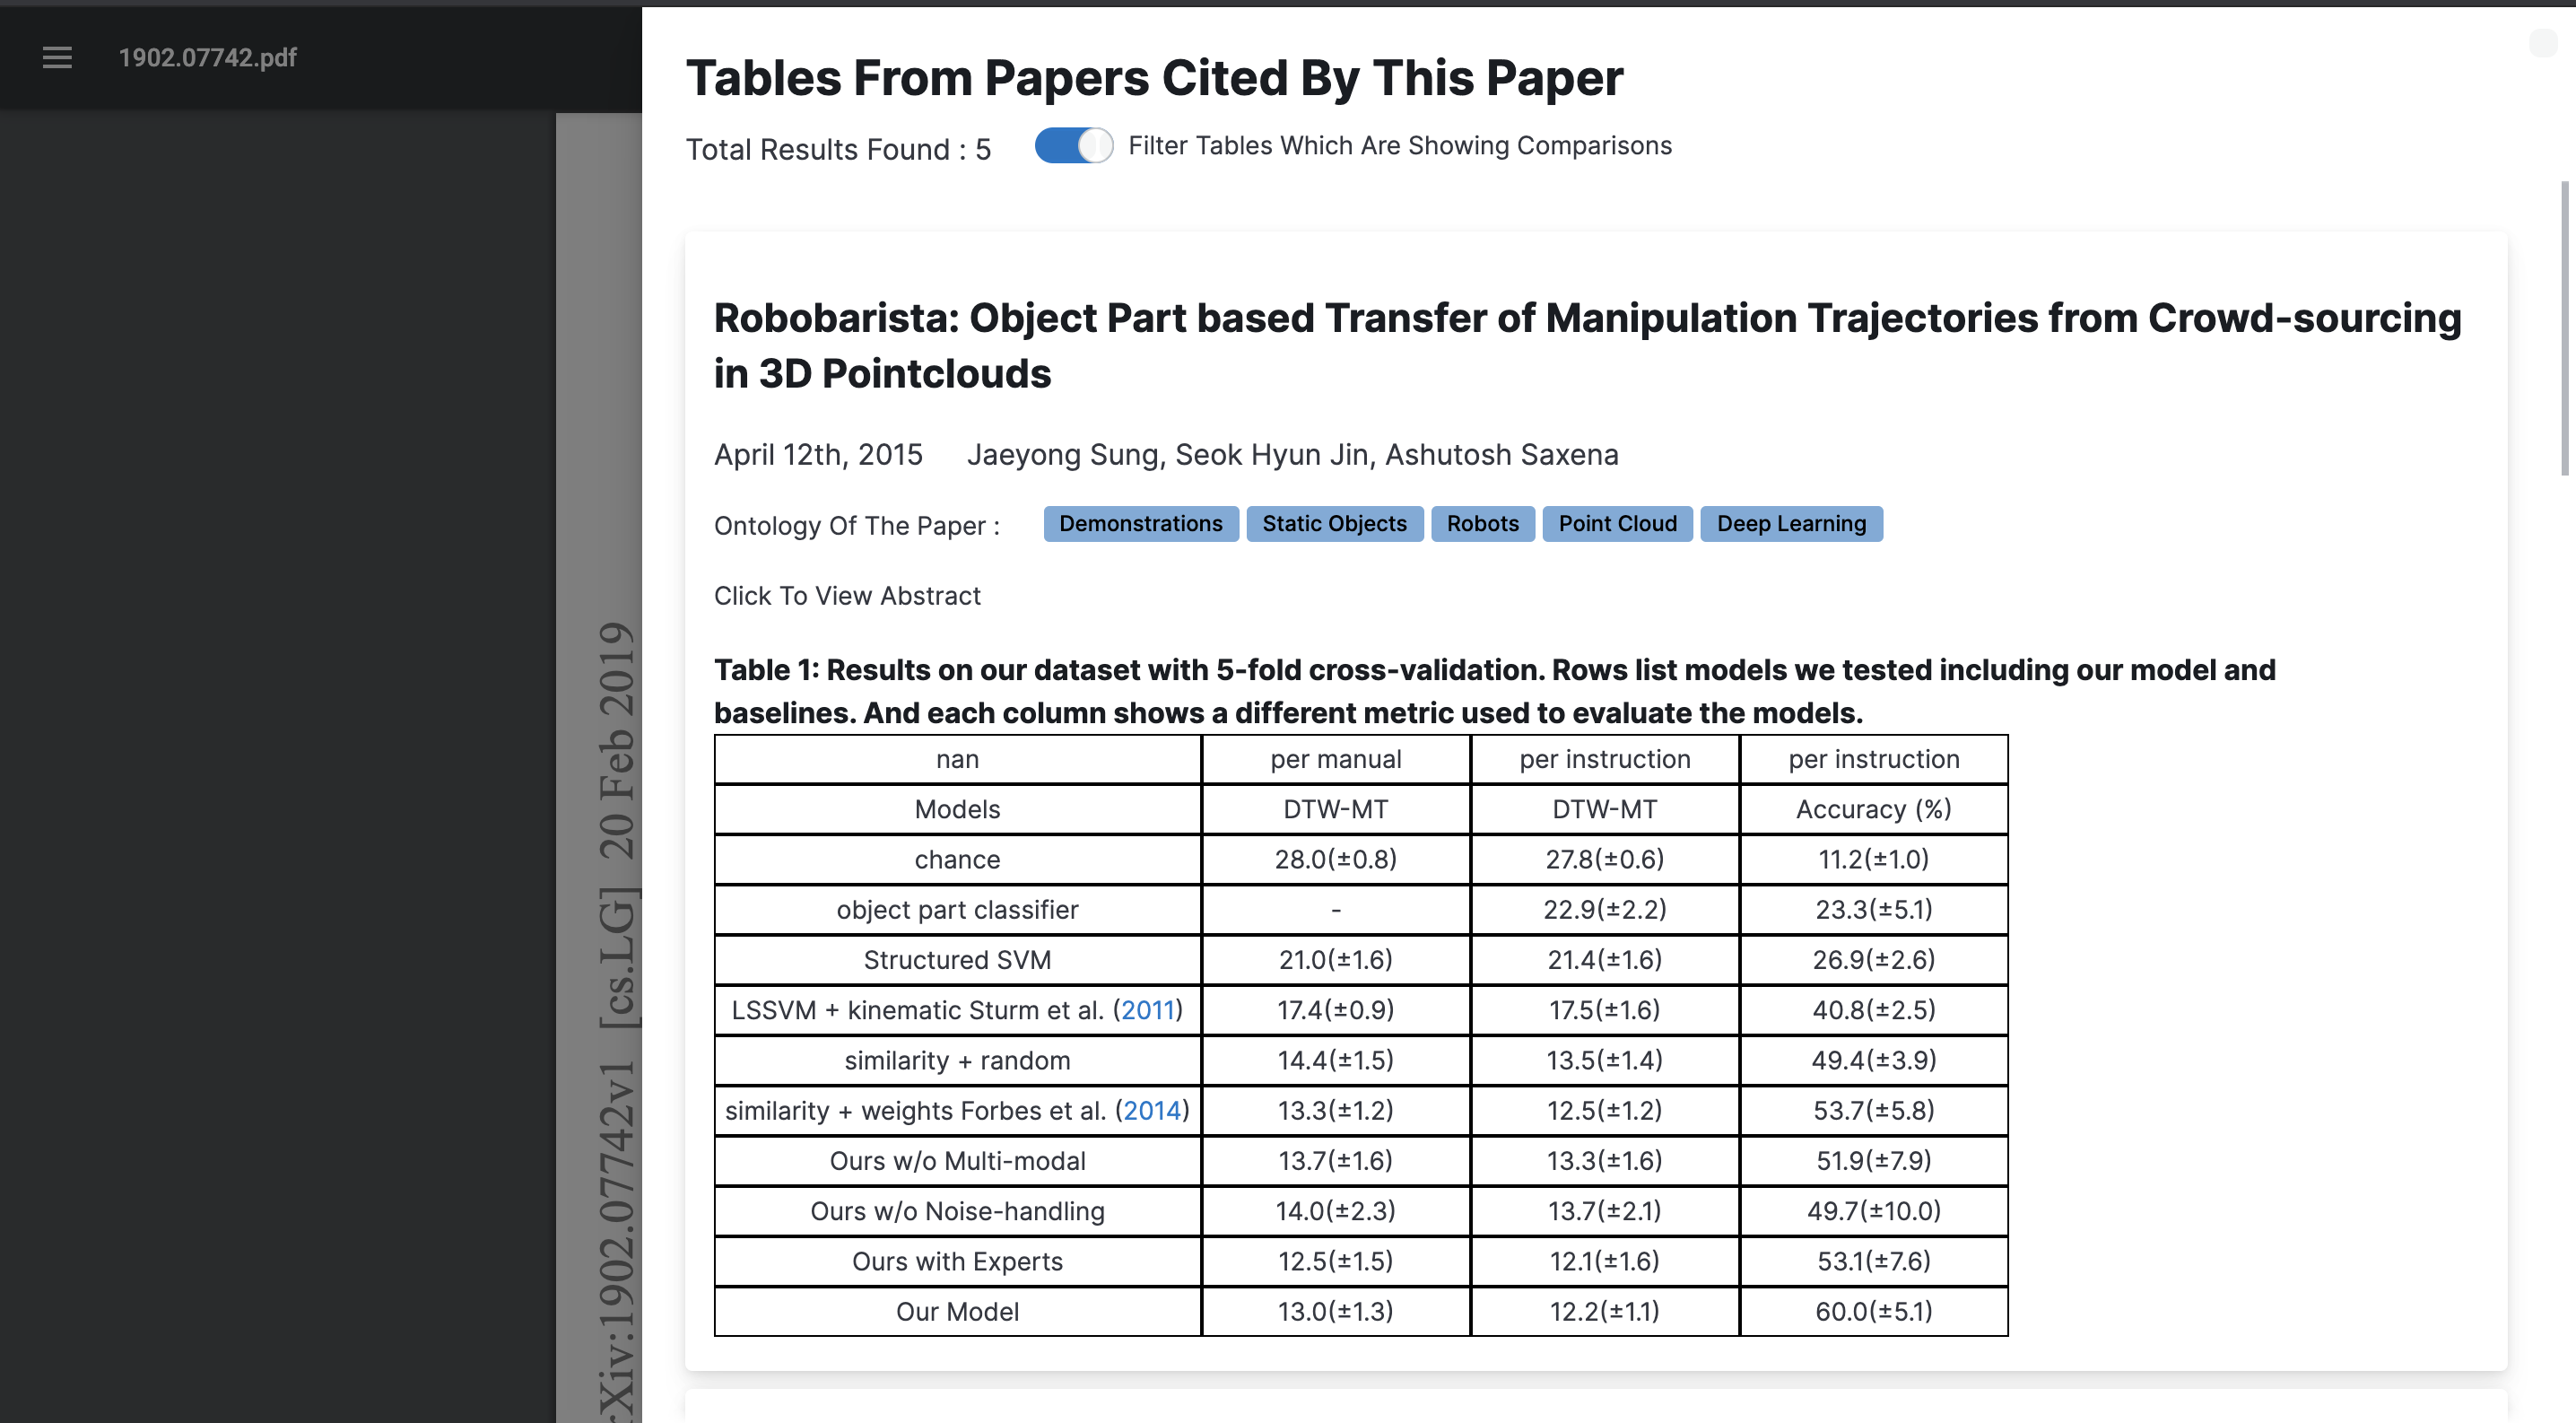
\includegraphics[width=\maxwidth{\textwidth}]{src/images/classification_exp.png}
    \caption{Tables describing comparisons filtered via API-Layer}
    \label{figure\arabic{figurecounter}}
\end{figure}
\refstepcounter{figurecounter}

The tables extracted from the papers that were cited also undergo a binary classification via a machine learning model to label the tables describing a comparison. This information is useful to provide context based filters at the time of reading, as seen Figure \ref{figure14}. Chapter \ref{table_classification} provides more details on the table of comparison classification and the choice of model for the API-Layer.
 
\subsection{Table Intent Labeling API}
The API Layer also provides API's for table annotation and labeling as seen in Figure \ref{figure15}. These annotations and labels help provide labeled data for the machine learning task which is discussed in Chapter \ref{table_classification}.


\chapter{Classifying Tables Describing Comparisons}
\label{table_classification}
A lot of valuable information about comparisons with some baselines and other research is present in the tables of academic research. Researchers tend to spend much valuable time finding the citations and the table of results from those citations. Sci-Genie via Citation Graph and the Machine Learning models helps filter tables describing comparisons at the time of reading research. 

This chapter will cover classifying tables that describe a comparison of entities and propose approaches to tackle the problem of classifying such types of tables. 

\section{Problem Formulation}

The structure of the tables in scientific research can fluctuate based on the information presented by the tables. The tables may also contain information whose context cannot be exactly inferred without the caption underneath the table. Tables occurring in scientific research can also be segregated into well-defined types such as the ones described in Chapter \ref{relatedwork:table-type}. These tables may also not contain a directly linkable entity from a knowledge base(KB) as entities defined in the research may not be present in the KB. Due to such different intrinsic characteristics, models trained using knowledge bases along with web tables such as the one by \cite{deng2020turl} cannot be directly fit to solve this problem. 

\begin{table}
    \label{table\arabic{tablecounter}}
    \centering
    \begin{tabular}{|l|l|l|}
        \hline
        Symbol & Meaning & Type \\ \hline
        $Y$ & Labels & Discrete : $\{0,1\}$ \\ \hline
        $X_T$ & Cell Embedding & $\mathbb{R}^{T_l \times d}$\\ \hline
        $X_C$ & Caption Embedding & $\mathbb{R}^{C_l \times d}$ \\ \hline
        $P_C$ & Positional Embedding & $\mathbb{R}^{C_l \times d}$ \\ \hline
        $E_r$ & Row Embedding & $\mathbb{R}^{T_l \times d}$ \\ \hline
        $E_c$ & Column Embedding & $\mathbb{R}^{T_l \times d}$ \\ \hline
        $T_l$ & Number Of Cells & $\mathbb{N}$ \\ \hline
        $T_r$ & Number Of Rows & $\mathbb{N}$ \\ \hline
        $T_c$ & Number Of Columns & $\mathbb{N}$ \\ \hline
        $C_l$ & Length of Caption & $\mathbb{N}$ \\ \hline
        $T_{cell}$ & Sequnces of Cells & $\mathbb{N}^{T_l}$ \\ \hline
        $f_\theta$ & Neural Network & - \\ \hline
    \end{tabular}
    \caption{\label{tablecounter} Table Of Symbols for Equations}
\end{table}
\refstepcounter{tablecounter}
The problem of classifying a table $T$ as a table describing a comparison can be framed as a binary classification problem. Given a table $T$ and its caption $C$, the classifier $f_\theta(T,C) \rightarrow Y$ predicts a binary label $Y \in \{0,1\}$ to denote weather the table is describing a comparison of entities\footnote{Both the table and caption are used because human labeling discovered that these two variables are the most prominant indicators of a table describing a comparison.}. 

Based on this formulation, this dissertation analyzes 4 different types of ML models and the representations they use for the table $T$ and caption $C$ for the problem:
\begin{itemize}
    \item Cross Channel Transformers With/Without Pretraining
    \item Encoder Only Multi-Channel Transformer With Pretraining
    \item Finetuning Pretrained Scibert
    \item SVM and Naive Bayes (Baselines)
\end{itemize}

Different models are analyzed because the representations of $T$ and $C$ can be treated as seperate variables or as a single variable based on the model. Cross Channel Transformer, Encoder Only Multi-Channel Transformer treats $T$ and $C$ as seperate representations, Scibert, SVM and Naive Bayes treats $T$ and $C$ as one joint representation. 

Section \ref{table_classification:models} describes the models developed/trained for the input representations of table $T$ and caption $C$. The data collection and labeling for the machine learning models is described in Section \ref{table_classification:data-coll}. The experiment results for different models is described in Section \ref{table_classification:experiement-result}

\section{Classification Models}
\label{table_classification:models}

\subsection{Encoder Only Multi-Channel Transformer}
\label{table_classification:models:encoder-model}
\begin{figure}[h]
    \centering
    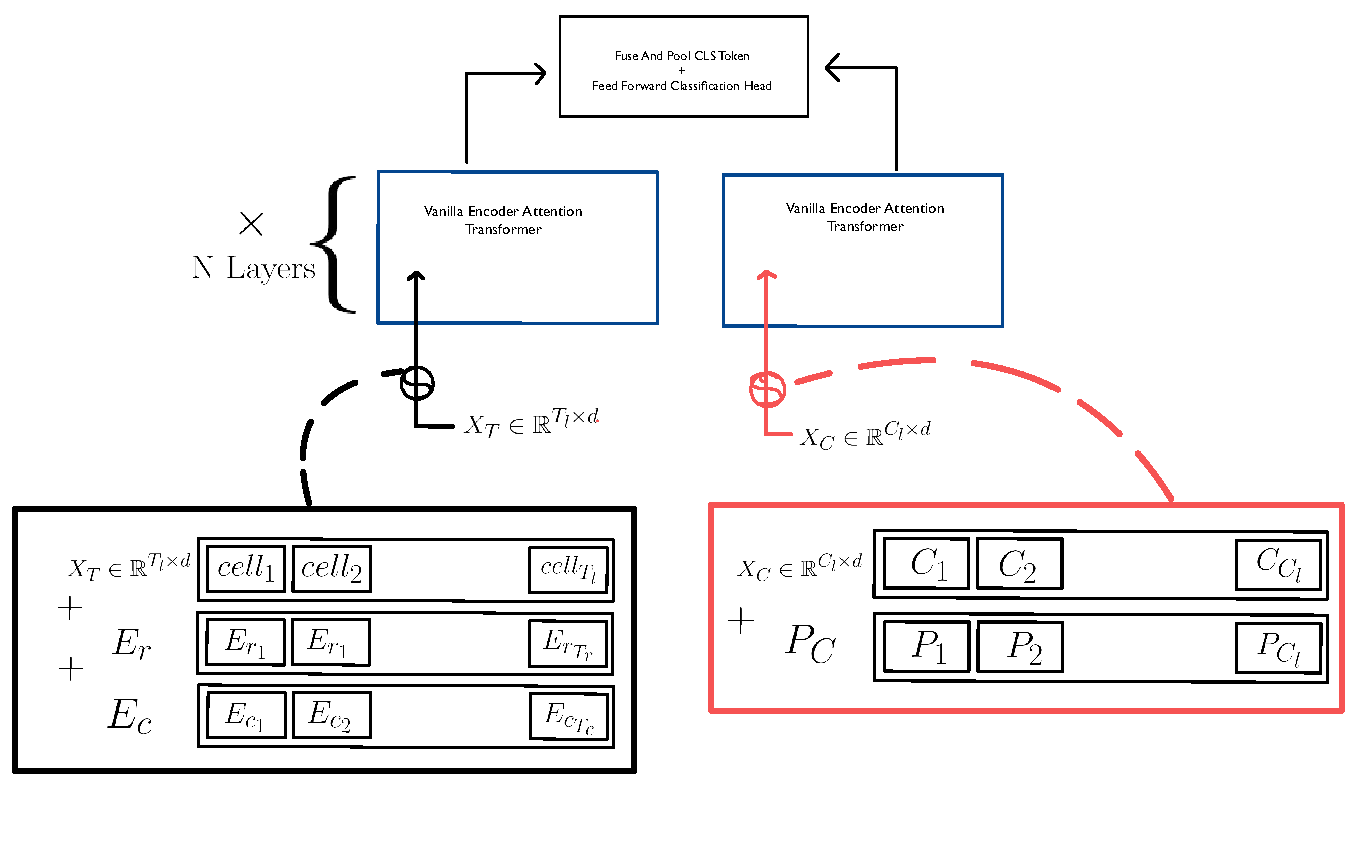
\includegraphics[width=\maxwidth{\textwidth}]{src/images/tabmod-enconly.pdf}
    \caption{Encoder Attention Transformer For Table Classification}
    \label{figure\arabic{figurecounter}}
\end{figure}
\refstepcounter{figurecounter}
Based on the models developed by \cite{deng2020turl}. A structurally-aware encoder only Transformer model is adapted to fit the function $f_\theta$. Figure \ref{figure17} visualises the model and its input representations.

\subsubsection{Input Representation}
\label{table_classification:models:encoder-model:input-rep}
Each table $T$ is represented as tuple of $(T_{cell},E_r,E_c)$; where $T_{cell} \in \mathbb{N}^{T_l}$ are the cells of the table represented as a sequence of integer tokens; $E_r$ is the row embedding where embedding $E_{r_{i}}$ represents the row of the cell $T_{cell_{i}}$ as an embedding;  $E_c$ is the column embedding where an embedding $E_{c_{i}}$ represents the column of the cell $T_{cell_{i}}$ as an embedding. The caption $C$ is represented as sequence of integer tokens which will be transformed to embeddings by the Transformer Model. The representations for the table $T$ are inspired from the models created by \cite{deng2020turl}. 

The cell sequence tokens $T_{cell}$ and caption $C$ are created using a word-piece tokenizer from the SciBert Model \footnote{https://huggingface.co/allenai/scibert\_scivocab\_uncased}. The tokenizer converts the value of individual cells or the caption into a sequence of integer tokens. These tokens can be used to create embeddings which are passed to the transformer model. 

\subsubsection{Model Description}
The table cell sequence $T_{cell}$ and the Caption $C$ are first converted to embeddings $X_T, X_C$ respectively. Post creation of the embeddings, the caption embedding  $X_C$ is added with the position embedding $P_C$; The cell embeddings $X_T$ are added with $E_r,E_c$. After the additions of the respective embeddings, differentiable CLS tokens are concatenated to $X_T,X_C$.

These embeddings are passed to individual encoder self-attention transformers. The class tokens from the final layer is pooled and sent for classification using a linear feed forward layer and a cross entropy loss is applied on the predictions. Figure \ref{figure17} visualizes the model. 


\subsection{Cross Channel Transformer}
\label{table_classification:models:cross-channel}
\begin{figure}[h]
    \centering
    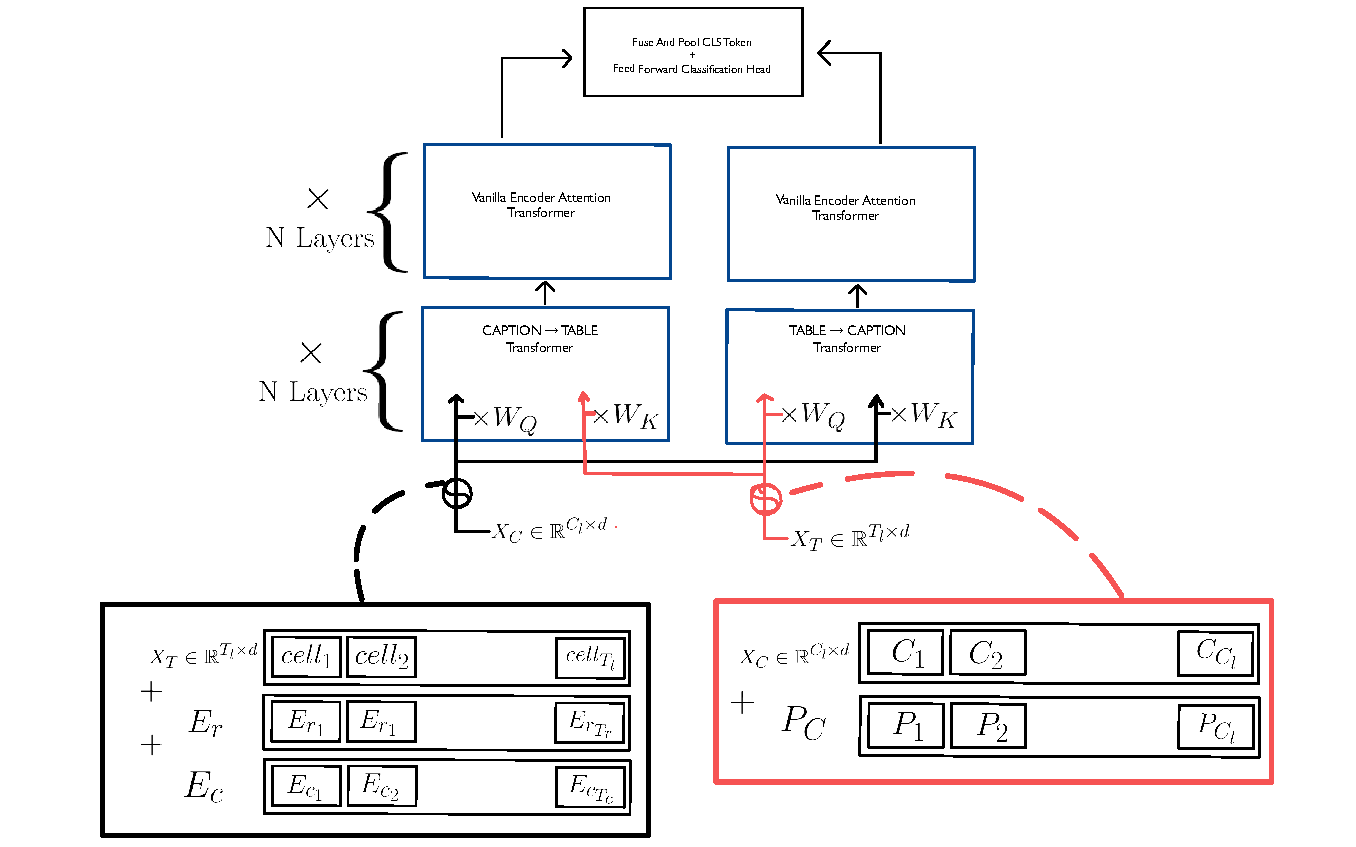
\includegraphics[width=\maxwidth{\textwidth}]{src/images/tablemodel.pdf}
    \caption{Cross Channel Transformer For Table Classification}
    \label{figure\arabic{figurecounter}}
\end{figure}
\refstepcounter{figurecounter}

Based on the models developed by \cite{tsai2019multimodal} and \cite{deng2020turl}, a structurally-aware cross channel Transformer model is adapted to fit the function $f_\theta$. Figure \ref{figure18} shows the outline of the model. This model is chosen to validate wheather cross attention will have an influence on the performance of the model if intermediate presentations for Table $T$ and Caption $C$ are generated from the cross attention operation. 

\subsubsection{Input Representation}
The input representations for $T$ and $C$ are the same as given in Section \ref{table_classification:models:encoder-model:input-rep}


\subsubsection{Model Description}
The table cell sequence $T_{cell}$ and the Caption $C$ are first converted to embeddings $X_T, X_C$ respectively. Post creation of the embeddings,  the caption embedding  $X_C$ is added with the position embedding $P_C$; The cell embeddings $X_T$ are added with $E_r,E_c$. After the additions of the respective embeddings, differentiable CLS tokens are concatenated to $X_T,X_C$.
These embeddings are passed to separate cross channel attention transformer layers \parencite{tsai2019multimodal} after which they are passed to the vanilla transformer encoder attention layers \parencite{vaswani2017attention}. Different strategies are chosen for handling the output of the vanilla tranformer encoder based on the type of task. 

Embeddings at the CLS token position, are pooled from the sequences and concatenated for the table of comparison classification task. Once concatenated, this joint embedding is passed to feed forward layers for classification using Cross Entropy Loss. For the pretaining task, the last vanilla encoder layer’s output will be used for predicting the masked tokens of the input table cells $T_{cell}$ and the caption $C$.

\subsection{Finetuning Scibert Transformer Model}
\cite{beltagy2019scibert} created a model which was trained on large full text corpus of scientific research containing 1.14M research papers. As this model has been subjected large amounts of pretraining, it is chosen for fine tuning for the same problem as the model may have encountered data of a similar distribution. 
\subsubsection{Input Representation}
\label{table_classification:models:sb:input_rep}
For the finetuning of SciBert, The Table $T$ and caption $C$ are serialized to strings and one concatenated string is created. An example representation is given below: 
\begin{verbatim}
    CAPTION : Table 1: Feature extraction time (Seconds), 
    number of parameters (Millions), and network size (Megabytes) 
    for each source on Office + Caltech-10 datasets.

    TABLE :                          0         1           2      3
0                     Task  Net size  Parameters   Time
1          Squeezenet [17]        46        1.24   13.3
2             Alexnet [21]       227          61   13.9
3           Googlenet [40]        27           7   15.9
4          Shufflenet [51]       6.3         1.4   17.0
5            Resnet18 [15]        44        11.7   14.8
6               Vgg16 [36]       515         138   33.6
7               Vgg19 [36]       535         144   37.1
8         Mobilenetv2 [35]        13         3.5   21.4
9        Nasnetmobile [55]        20         5.3   39.3
10           Resnet50 [15]        96        25.6   22.7
11          Resnet101 [15]       167        44.6   26.7
12        Densenet201 [16]        77          20   61.8
13        Inceptionv3 [41]        89        23.9   28.2
14            Xception [4]        85        22.9   48.1
15  Inceptionresnetv2 [39]       209        55.9   54.1
16        Nasnetlarge [55]       360        88.9  141.2
\end{verbatim}

\subsubsection{Model Description}
The input representation string is converted to a sequence of integer tokens which are capped to the length of 512 tokens because of SciBert's constraint on maximum sequence length. A class token is added at the start of the sequence; the sequence is then passed to the Scibert Model. The class token is pooled from after the final layer and is passed to a feed forward neural network for binary classification using cross entropy loss. 


\subsubsection{Model Training}
The model is trained using the for 6 epochs with a linear learning rate warm up schedule of 20 epochs.

\subsection{Baselines}
SVM models are used as baselines as when \cite{kim2012scientific} conducted a study for table type classification, deep learning was not as popular. Naive Bayes(NB) model are also chosen as an additional baseline for the classification task. 

\subsubsection{Input Representation}
The input representation for the SVM and the NB model are the same as the string described in Section \ref{table_classification:models:sb:input_rep}. The string undergoes tokenisation and a classifier is trained based on TF/IDF values of the input strings. 

\subsection{Pretraining Transformers}
\label{table_classification:models:encoder-model:pre-train}
Based on the insights learned from \cite{hernandez2021scaling} on the effectiveness of pretrained models for downstream tasks, the cross-channel transformer model is pretrained with 70K tables from papers from ArXiv. A masked language modeling pretraining objective is used to train the Transformer model given in Figure \ref{figure18}, and \ref{figure17}. The pretraining follows the procedures described by \cite{deng2020turl} where the task is of Mask Language Modeling(MLM) for the sequence of cells $T_{cell}$ and the caption $C$. The model is tasked to predict the word token where a MASK token is inserted in the table $T$ and caption $C$. A mask is inserted in 80\% of the training samples with 15\% of the sequence being masked. The cross entropy losses from MLM predictions of the Table and Caption is added and backpropagated. 

This objective allows training the model with large number of tables instead of using classifiers trained on small amounts of data. The pretraining task is run for 35K steps in 5 epochs. The learning rate is set to 0.0001 for the pretraining task with an AdamW optimizer. Both the transformer models described in Section \ref{table_classification:models:encoder-model}, \ref{table_classification:models:cross-channel} are pretrained using the same MLM objective. 

\subsection{Finetuning Transformers}
After the Cross Channel Transformer and the Encoder Only Multi-Channel Transformer undergo the pretrainig task; the models are finetuned on the classification task with a learning rate of 2e-05, scheduled with a linear learning rate scheduler for 20 epochs using the AdamW optimizer. 

\section{Data Collection And Labeling}
\label{table_classification:data-coll}

\begin{figure}[h]
    \centering
    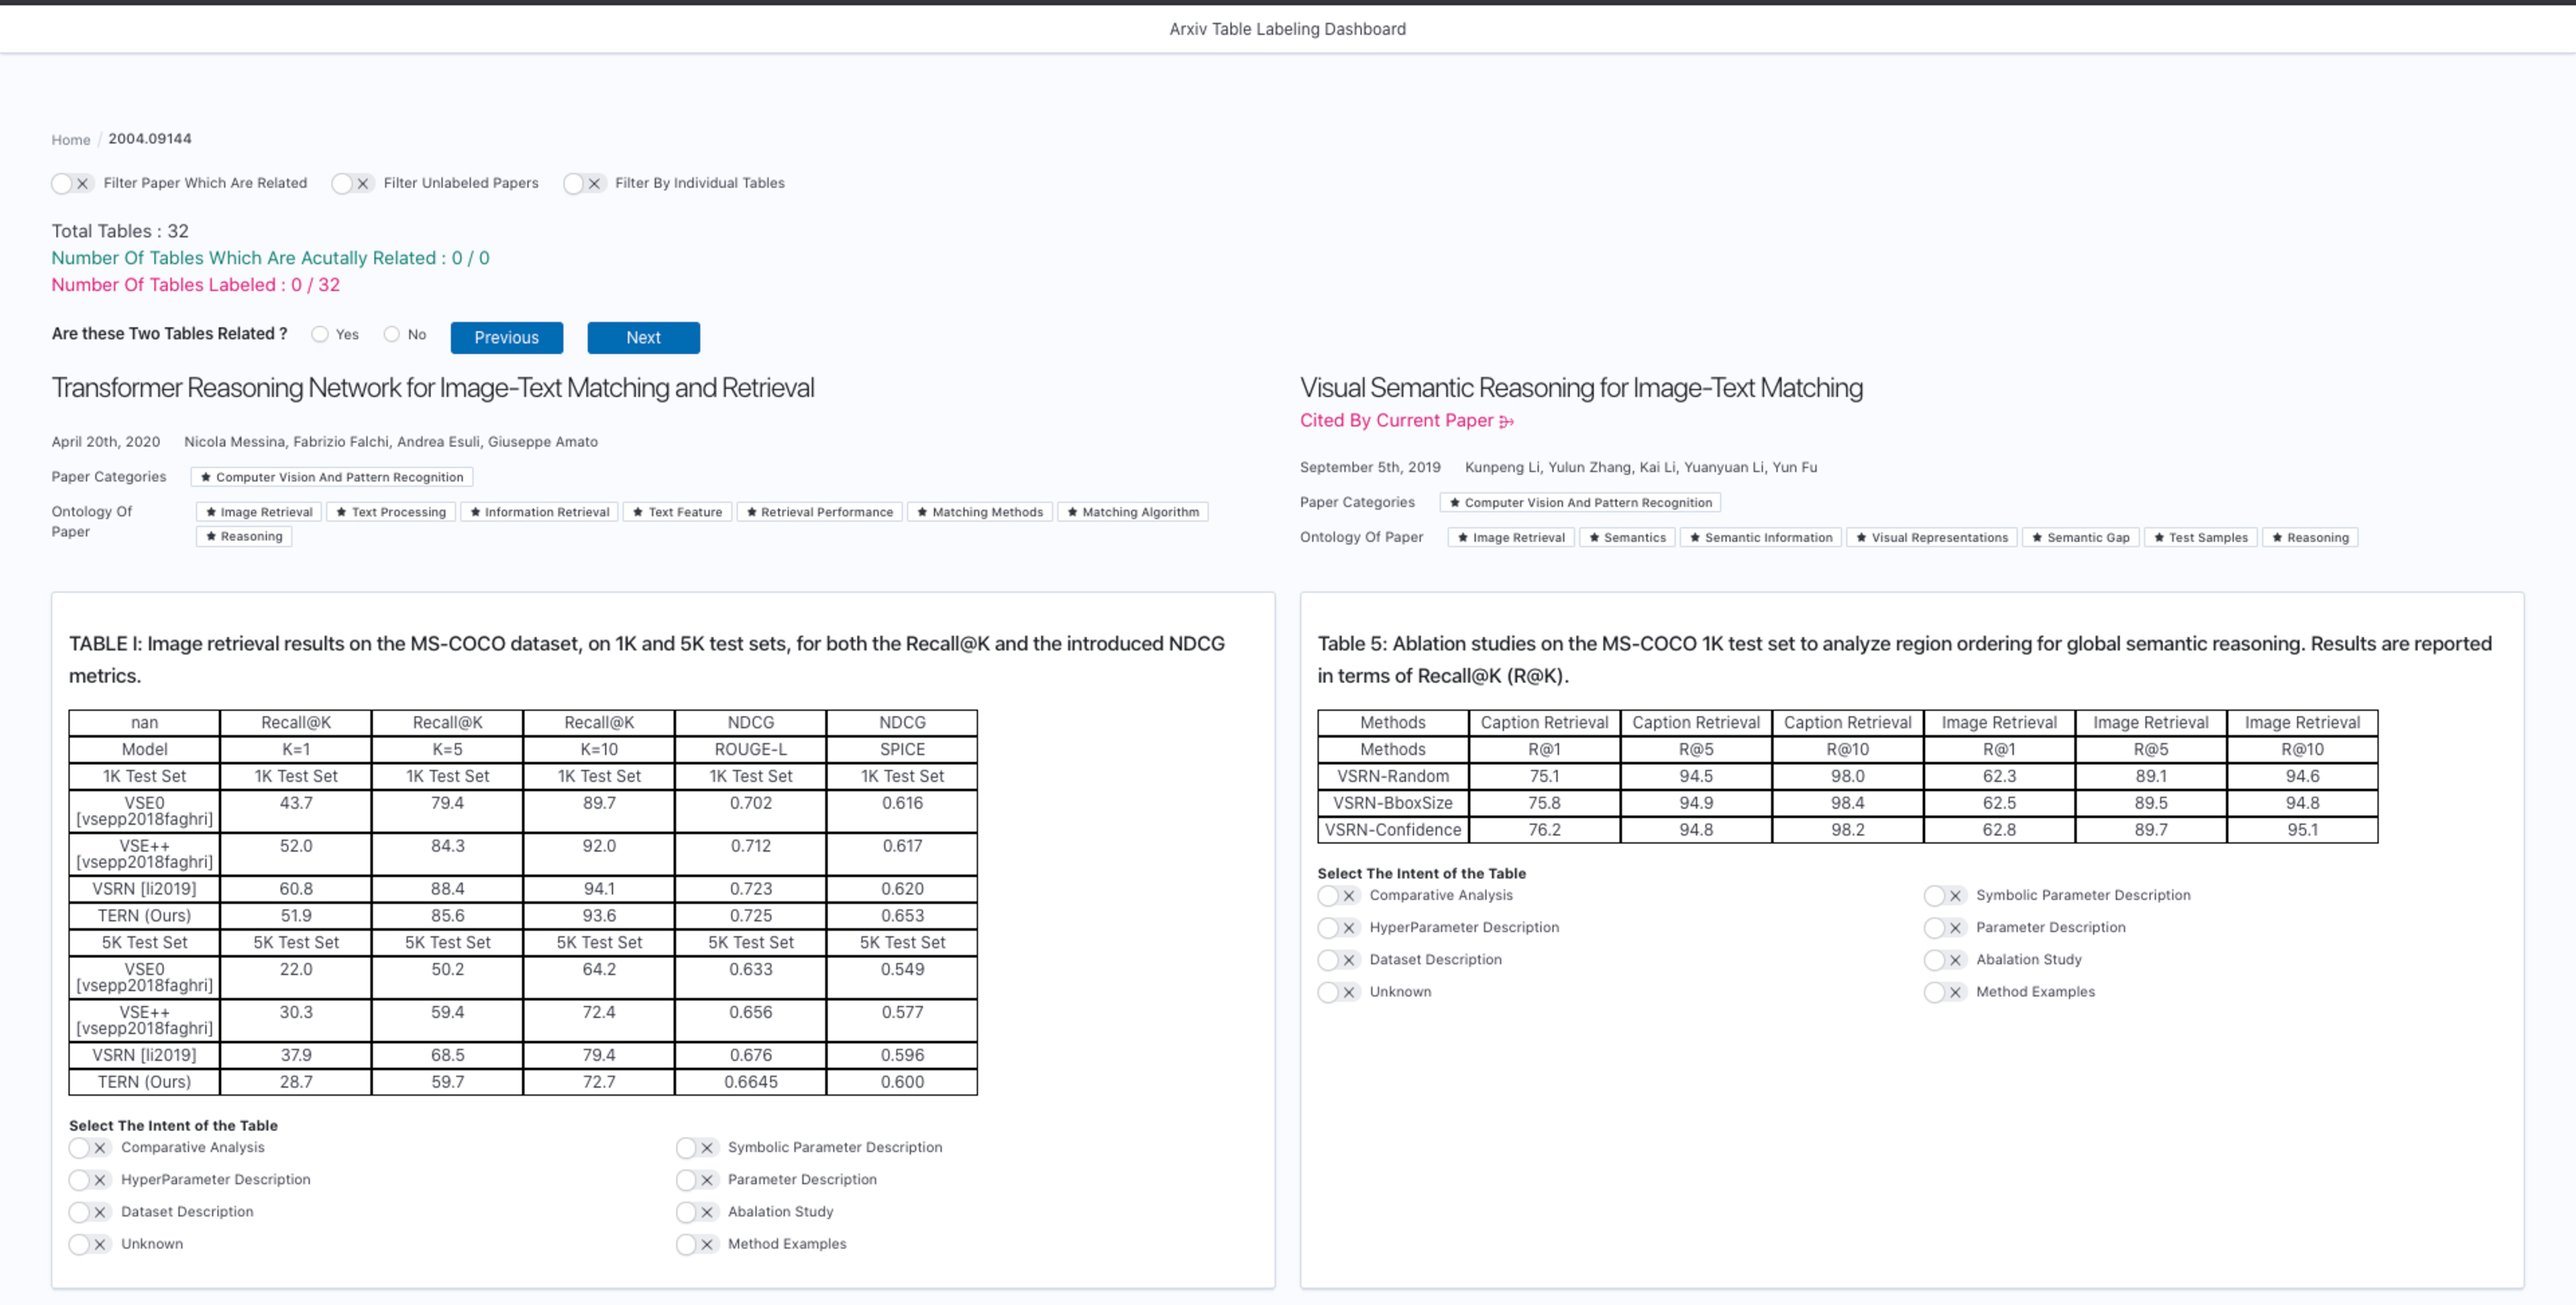
\includegraphics[width=\maxwidth{\textwidth}]{src/images/table-lable-exp.pdf}
    \caption{Table Labeling Interface For Table Relation and Intent Annotation}
    \label{figure\arabic{figurecounter}}
\end{figure}
\refstepcounter{figurecounter}

As Sci-Genie consists of a Data Layer (Chapter \ref{sci-genie-core:data-layer}) that contains the tables from the research papers, A labeling interface(Figure \ref{figure16}) is designed to annotate tables from 240 research papers. 820 tables are annotated out of which 574 tables are describing a comparison and 246 are not. The labeling interface supports labeling types to tables described by \cite{kim2012scientific} and few more based on the observations from current CS research. More details regarding this subject are discussed in Chapter \ref{conclusion:future-scope:type-class}. 

\section{Experiment Results}
\label{table_classification:experiement-result}
\begin{figure}[h]
    \centering
    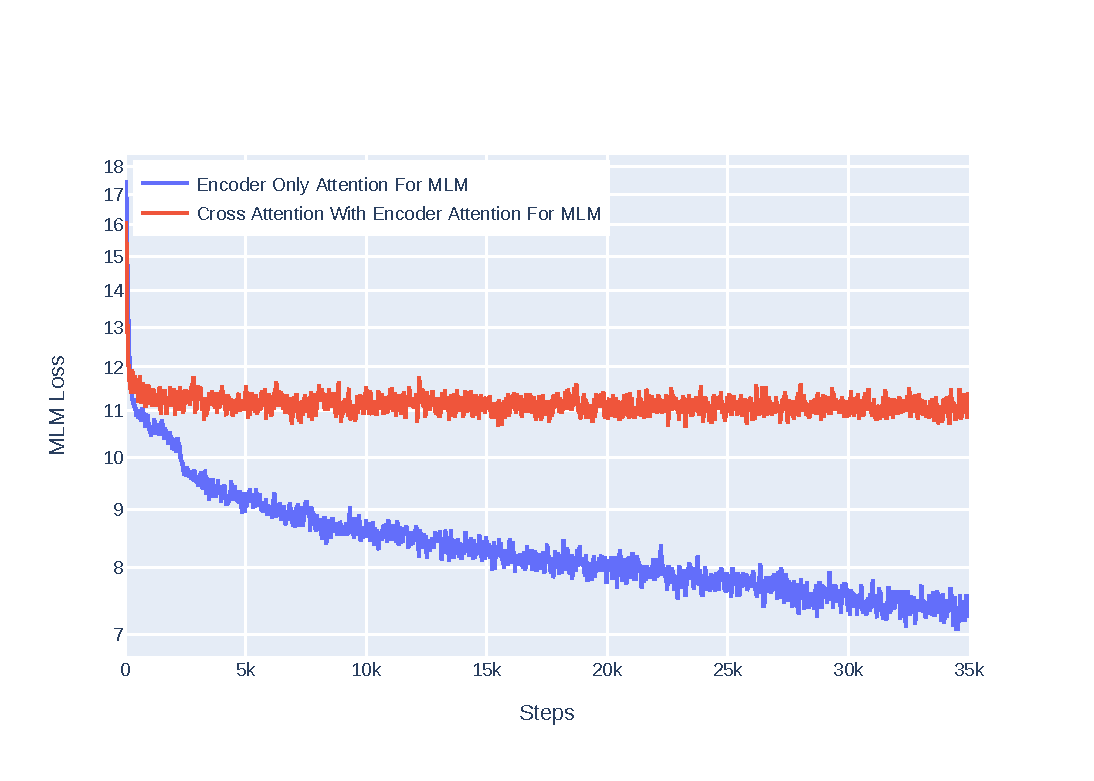
\includegraphics[width=\maxwidth{\textwidth}]{src/images/mlm-loss-comparison.pdf}
    \caption{Masked Language Modeling(MLM) Loss For Encoder Style Attention VS Cross Attention. The MLM losses for $T$ and $C$ are summed}
    \label{figure\arabic{figurecounter}}
\end{figure}
\refstepcounter{figurecounter}

\begin{table}[h]
    \label{table\arabic{tablecounter}}
    \centering
    \begin{tabular}{|p{4cm}|p{3cm}|p{3cm}|p{3cm}|}
    \hline
        \textbf{Model} & \textbf{Accuracy} (\%) & \textbf{F1 Score}  & \textbf{Loss} \\ \hline
        Naive Bayes & 71.6 & 0.825 & - \\ \hline
        SVM  & 78.39 & 0.85477 & - \\ \hline
        Cross Channel Transformer From Scratch (31M) & $73.95 \pm 10.5 $ & $0.739 \pm 0.107$ & $0.53 \pm 0.08$ \\ \hline
        Encoder Only Multi-Channel Pretained (25M) & $88.33 \pm 0.29$ & $0.8883 \pm 0.002$ & $0.423 \pm 0.007$ \\ \hline
        Cross Channel Transformer Pretained (31M) & $87.5 \pm 1.8$ & $0.875 \pm 0.018$ & $0.34 \pm 0.016$ \\ \hline
        SciBert Finetuned (112M) & $92.23 \pm 1.60$ & $0.923 \pm 0.016$ & $0.21 \pm 0.04$ \\ \hline
    \end{tabular}
    \caption{\label{tablecounter} Test set results of the table classification models using SOTA Transformer and baselines. Average Results from 4 Training runs is reported}
\end{table}
\refstepcounter{tablecounter}
The following are the experiment and their conditions for ML model training:
\begin{itemize}
    \item Cross Channel Transformer: Pretrained with 70K Tables and finetuned on the classification task
    \item Cross Channel Transformer: Directly trained from scratch on the classification task 
    \item Encoder Only Multi-Channel Transformer : Pretrained with 70K Tables and finetuned on the classification task
    \item SciBert: Finetuned on the classification task.
    \item Naive Bayes \& SVM
\end{itemize}
More details on the hyperparameters for the experiments are found in the Appendix \ref{appendix:toc}. All experiments are conducted on the same frozen test set with evenly balanced samples. Numbers are reported after averaging 4 training runs.

All experiments are conducted using Google Colab Notebooks on NVIDIA P100 GPUs. Table \ref{table5} describes the results of the experiments. 

The pretrained models perform substantially better than the baselines. The Cross-Channel Tranformer when pretrained from scratch performs substantially better than the model trained from scratch. The Encoder Only Multi-Channel Transformer performs the best among all the models pretrained on ArXiv Tables. SciBert outperforms all models. The reason for Sci-Bert's better performance can be inferred based on the study by \cite{hernandez2021scaling}. As SciBert is a much bigger model, trained on a very large corpus consisting of data from a similar distribution, its performance would be better than the baseline and the developed models. It can also be seen from Table \ref{table5} that pretraining has a direct influence on a better model compared to training the model from scratch. 
\chapter{Conclusion and Future Scope}
\label{conclusion}

\section{Sci-Genie: Technical Debts and Shortcomings}
Although Sci-Genie provides a more context rich access to research, the components that help enrich context during search and parsing/indexing can be further improved. This section details the limitations of some components. Based on some of these limitations, future works is described in Section \ref{conclusion:future-scope}

\subsection{Heuristic Parsing}
\begin{figure}[h]
    \centering
    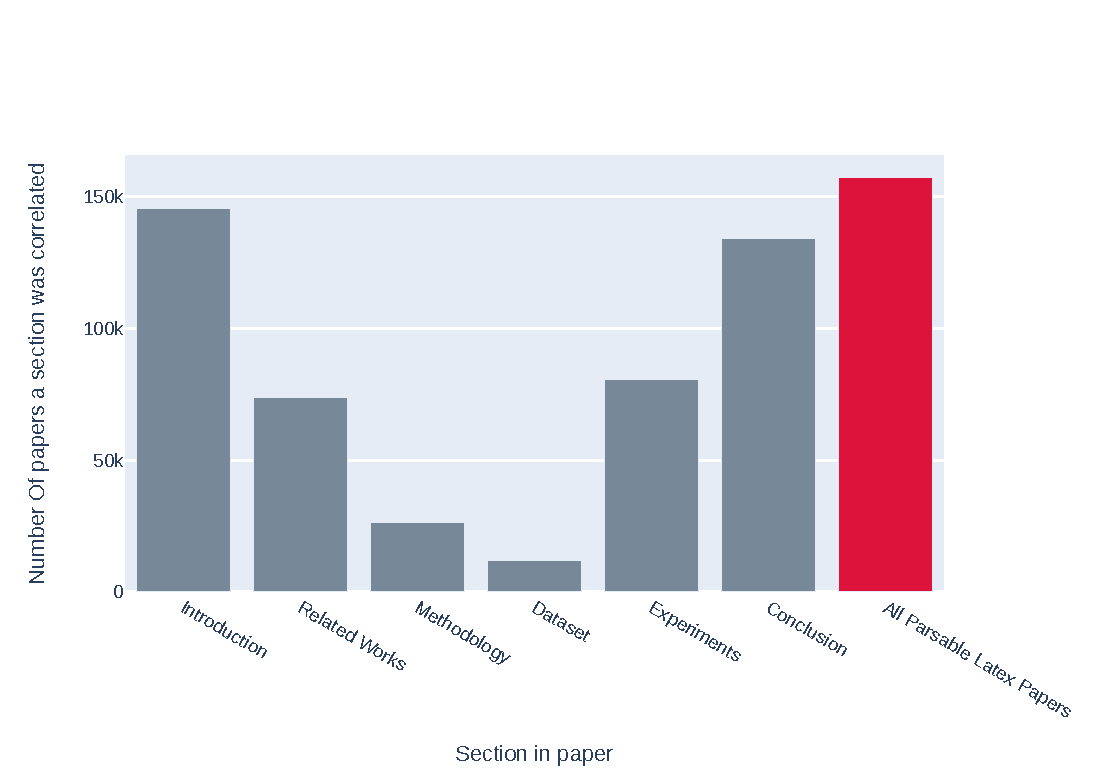
\includegraphics[width=\maxwidth{\textwidth}]{src/images/parsing-stats.pdf}
    \caption{ A bar plot of number of documents where a section got parsed by the heuristic parser from 158K papers}
    \label{figure\arabic{figurecounter}}
\end{figure}
\refstepcounter{figurecounter}
As Sci-Genie uses a heuristic parser for parsing research documents. The heuristic parser correlates the Fragment object to the appropriate keys in the \nameref{sci-genie-core:data-layer:researchobj}. Figure \ref{figure18} shows the statistics of parsing using the heuristic parser from a total corpus of 158K papers. As the parser misses out many sections it can be further improved using better methods. The parser also considers the sections based on ones observed in CS papers. Future research directions can include identifying common patterns in the structure of research documents for fields outside CS; the identified structure can be used for providing additional context to search results. 


\subsection{LaTeX only Parsing}
Sci-Genie doesn't parse PDF and uses Latex instead. A lot of research in other fields is present in PDF and Sci-Genie doesn't have PDF mining capabilities. 

\subsection{CS ArXiv Only Access}
While ArXiv can be a source of freely availability well cited research, it also remains a preprint server where all documents are not gauranteed to be cited. Sci-Genie only supports CS ArXiv articles and its ontology is specialized for CS research. Future versions can extend the search engine to support more fields of research and use ontology for those fields. 

\section{Future Research Scope}
\label{conclusion:future-scope}
\subsection{Grannular Table Type Classification}
\label{conclusion:future-scope:type-class}

The table types defined by \cite{kim2012scientific} are general purpose descriptions which can apply to various domains. Although they are quite useful, tables in recent CS literature have more grannular sub-classifications. For example a "Statistics Table" could be describing a Dataset for Machine Learning experiments. The tables which may seem as Experiments Results can also be describing an Ablation Study conducted on a ML model. Due to a very nuanced distinction between a lot of these tables, The task of machine learning to classify table types needs more grannular sub-types within the classes defined by \cite{kim2012scientific}. 

Multiple grannular table types such as Ablation Study, Dataset Descriptions, can also be further described based on the field of research the tables belong to. The interface shown in Figure \ref{figure17}, was developed to annotated tables from scientific research. This interface can be extended for many fields outside CS for the effort of curation and benchmarking of ML models for indentification of various types of tables from different avenues of research. 

\subsection{Discovering Related Tables}
\begin{figure}[h]
    \centering
    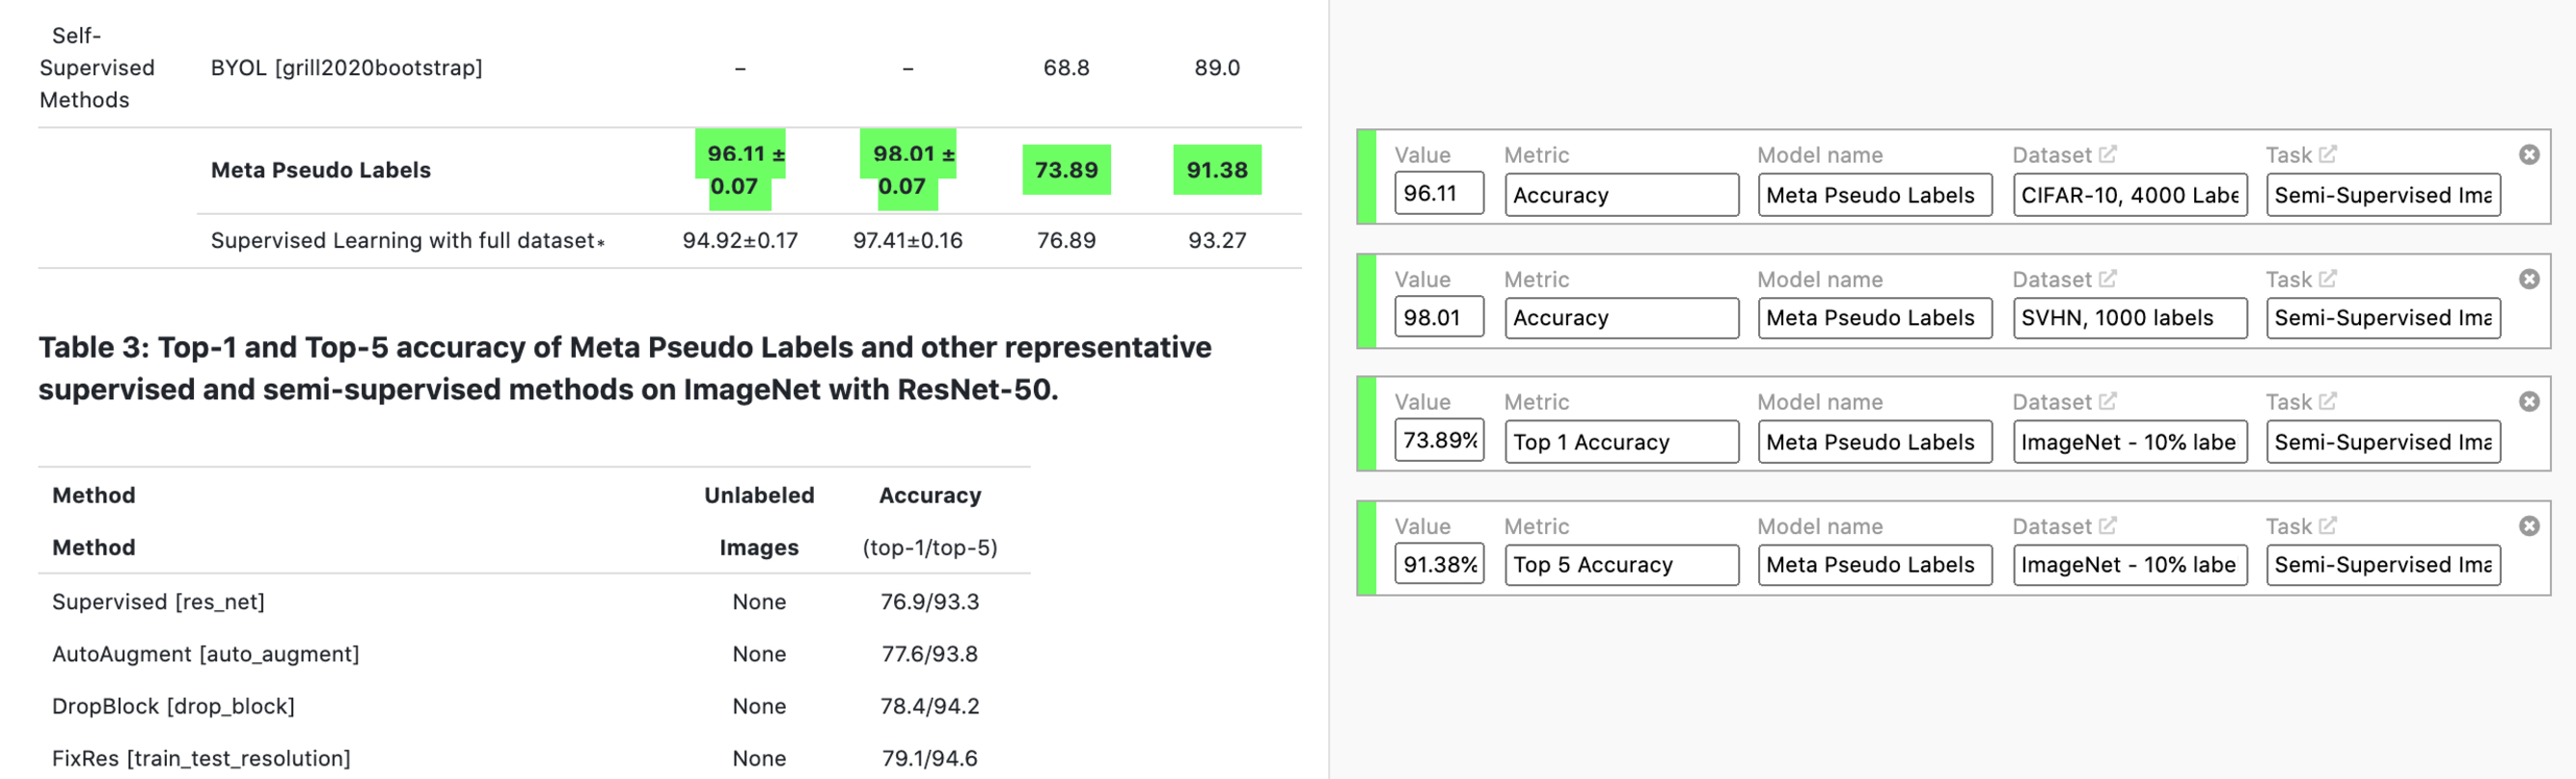
\includegraphics[width=\maxwidth{\textwidth}]{src/images/pwc-table-exp.pdf}
    \caption{ Viewing Tables From SOTA benchmarks }
    \label{figure\arabic{figurecounter}}
\end{figure}
\refstepcounter{figurecounter}
Organisations such as PapersWithCode(PwC) have developed tools to collate information about SOTA ML methods from papers on ArXiv. PwC after parsing these tables either correlate some metrics manually and some intelligently via the use of libraries like Axcell\footnote{https://github.com/paperswithcode/axcell}. This task can become more intelligent and automated where ML models can be developed to correlated tables from research documents from diverse domains outside CS. Discovering related tables using a citation graph and machine learning techniques can be a great direction for future research. 

\subsection{Scientific Research Document Parsing For Search Context}
Google search pivoted to ranking results for search using BERT.\footnote{https://blog.google/products/search/search-language-understanding-bert/} since 2019. This trend of using language models to help rank search results has lead to creation of opensource tools\footnote{https://github.com/deepset-ai/haystack} over off the shelf search engines like Elasticsearch. Although the models help improve search ranking, more nuanced search context result information is yet not accessible via academic research search engines. 

Intelligent parsing maybe one part of the solution. Sci-Genie are uses domain sepecific content parser which is heuristically derived (Chapter \ref{sci-genie-core:scraping:frag-to-rs}) to help bring context relevant information in search results. This parser may not be extensible to various other domains or document types.

\cite{kashyap2020sciwing}, introduced deep learning based techniques for scientific document parsing. But parsing can also be posed a domain specific problem where each domain generally follows a different parse structure. For example, recent papers in Machine Learning explicitly discuss datasets as a section in the paper.

Every domain's specific nuances requires more intelligent systems that can learn to identify such traits on their own. Intelligent techniques of parsing and indexing data to provide sufficient context to the users seems a rich direction of research in the future.

\section{Conclusion}
The fast rate of growth in technological progress will dramatically increase the growth in the volume of research in the future. Figure \ref{figure1}, is the best proof of that insight. The growing volume of research would also require more nuanced search tools which can help surface enough context around search terms and futher aid the researcher when reading research. This dissertation described a search engine and browser app based prototype solution to help remediate this problem. This dissertation covered the formulation of different aspects of the search engine and the ML models powering its table of comparison filtering algorithm. 

In summary, the proposed solutions in this dissertation try to remediate the problem of growth in the volume of research by aiding the researcher with more context based information when searching for research and reading research.

%\include{chapter2}                     %   \include rather than \input for chapters
%\include{chapter3}% etc.
                                        % Heading commands (in descending order):
                                        % \chapter
                                        % \section
                                        % \subsection
                                        % \subsubsection
                                        % \paragraph
                                        % \subparagraph

%%%%%%%%%%%%%%%%%%%%%%%%%%%%%%%%%%%%%%%
% Back matter
%%%%%%%%%%%%%%%%%%%%%%%%%%%%%%%%%%%%%%%
\SingleSpacing                          % Back matter should be single spaced
\AfterEndEnvironment{table}{\SingleSpacing} % Reset these environments
\AfterEndEnvironment{figure}{\SingleSpacing}
\AfterEndEnvironment{quote}{\SingleSpacing}
\AfterEndEnvironment{quotation}{\SingleSpacing}

\edef\defaulttolerance{\the\tolerance}
\tolerance 500                          % Increase tolerance to prevent material extending into margins
\hbadness 500

\iftoggle{useendnotes}{%                % If you're using endnotes, output them here
  \setsecnumdepth{none}                 % No section numbering in end notes
  \bookmarksetup{startatroot}           % Make Notes appear at root level of PDF bookmarks
  \phantomsection%                      % Need for hyperref
  \addcontentsline{toc}{chapter}{%      % Add a chapter-level heading for
    \hspace{-\cftchapterindent}%        %  Notes to the ToC
    \notesname%
  }%
  \renewcommand*{\notedivision}{%
    \chapter*{\notesname}%
  }
  \printpagenotes                       % Output the notes
  \setsecnumdepth{all}%                 % Turn section numbering back on after printing
}{}

\bookmarksetup{startatroot}
\chapter*{\bibheading}                  % In the running text, use a chapter-level heading
                                        % for the bibliography section
\phantomsection
\addcontentsline{toc}{chapter}{%        % In the TOC, add a custom chapter-level heading
  \hspace{-\cftchapterindent}%          % that will be flush against the left margin
  \bibheading%
}
%\phantomsection
%\addtocontents{toc}%                    % Add this 'mark' to TOC so subsequent pages use
%  {\protect\markboth{\bibheading}{Page}}%   the bibliography heading (unlikely since
%                                        %   the appendices follow quickly)
\iftoggle{usebiblatex}{%                % Output the bibliography
  \printbibliography[heading=none]      % Using a 'biblatex' package; do not let
                                        %   'biblatex' output a heading
}{%
  \renewcommand\bibsection{}            % Do not let 'natbib' output a heading
  \bibliographystyle{\natbibstyle}      % Using 'natbib' to print bibliography
  \bibliography{\bibfilename}
}

\appendix                               % Indicate start of appendices
                                        % Appendices are considered 'mainmatter' in this
                                        %   documentclass
\tolerance \defaulttolerance            % Set tolerance back to default
\hbadness \defaulttolerance

\addtocontents{toc}{\protect%           % Only include appendix title in table of contents
  \setcounter{tocdepth}{0}}%            %   and omit sub-headings
\renewcommand*{\chapnamefont}%          % Reset font for 'Appendix' in chapter titles
    {\normalfont\MakeTextUppercase}
\makeatletter                           % Clear page after printing appendix title
  \renewcommand{\memendofchapterhook}%
  {%
    \clearpage
    \m@mindentafterchapter
    \@afterheading
  }
\makeatother

\phantomsection                         % Need '\phantomsection' to place hyperref
                                        %   bookmark more accurately
\addcontentsline{toc}{part}{Appendix}   %~Add "Appendix" to TOC here; comment out this
                                        %   line if you're not including appendices

\phantomsection                        %!This is the one part of the template that I
\addtocontents{toc}%                   %   could not get to work properly. After you
 {\protect\markboth{APPENDIX}{Page}}  %   start listing appendices in the TOC,
                                        %   subsequent TOC pages should use "APPENDIX in
                                        %   the header instead of "CHAPTER"; however,
                                        %   this code will make "APPENDIX" appear on the
                                        %   the same page that the *first* appendix
                                        %   appears on. This problem won't affect most
                                        %   people, but if it affects you, uncomment
                                        %   these lines and move them below where
                                        %   the appendices are listed. Keep moving these
                                        %   lines down and checking the output until
                                        %   the TOC headers appear correctly

%\include{appendix1}                     %~Insert your appendices here; I recommend to use
%\include{appendix2}                     %   \include rather than \input for appendices.
%\include{appendix3}% etc.               %   All heading commands are the same as above,
                                         %   e.g., \chapter, \section, etc.

% \chapter{Appendix}
\chapter{Elasticsearch Related Information}
\section{Arxiv Parsed Research Index Example}

\begin{verbatim}
 {
    "identity": {
      "identity": "2104.00682",
      "url": "http://arxiv.org/abs/2104.00682v1",
      "title": "",
      "abstract": "",
      "categories": [
        "cs.CV",
        "cs.AI",
        "cs.LG"
      ],
      "published": "2021-04-01T17:59:48Z",
      "updated": "2021-04-01T17:59:48Z",
      "authors": [
        "Bo Xiong",
        "Haoqi Fan",
        "Kristen Grauman",
        "Christoph Feichtenhofer"
      ],
      "affiliation": [],
      "version": 1,
      "journal_reference": null,
      "created_on": "2021-04-02T04:20:33.981856"
    },
    "research_object": {
      "introduction": {
        "name": "Introduction",
        "subsections": [],
        "text": "",
        "matched": true
      },
      "related_works": {
        "name": "RelatedWorks",
        "subsections": [],
        "text": "",
        "matched": true
      },
      "methodology": {
        "name": "Methodology",
        "subsections": [],
        "text": "",
        "matched": false
      },
      "experiments": {
        "name": "Experiments",
        "subsections": [],
        "text": "",
        "matched": true
      },
      "results": {
        "name": "Results",
        "subsections": [],
        "text": "",
        "matched": false
      },
      "dataset": {
        "name": "Dataset",
        "subsections": [],
        "text": "",
        "matched": false
      },
      "conclusion": {
        "name": "Conclusion",
        "subsections": [],
        "text": "",
        "matched": true
      },
      "limitations": {
        "name": "Limitations",
        "subsections": [],
        "text": "",
        "matched": false
      },
      "unknown_sections": [
        {
          "name": "",
          "subsections": [
            {
              "name": "",
              "subsections": [],
              "text": ""
            }
          ],
          "text": ""
        }
      ]
    },
    "parsing_stats": {
      "active": true,
      "section_matches": [
        "Introduction",
        "RelatedWorks",
        "Experiments",
        "Conclusion"
      ],
      "num_un_matched": 2
    },
    "created_on": "2021-04-02T04:20:40.318679",
    "ontology": {
      "syntactic": [
      ],
      "semantic": [
      ],
      "union": [
      ],
      "enhanced": [
      ],
      "mined": true
    }
  }
\end{verbatim}

\section{Content Parsing Code/Algorithm}
\label{appendix:content-parsing-code}
The \textit{ArxivLatexParser} is used to create the parsed content tree from which section based correlation is done. Below is the algorithm and source code in Python programming language.
\begin{lstlisting}
  
import os 
from subprocess import Popen, PIPE
from tex2py import tex2py 
from typing import List
import json


def get_tex_tree(tex_path):
    with open(tex_path,'r') as f:
        data = f.read()
    tex_root_node = tex2py(data)
    return tex_root_node

class Section():
    """Section 
    Section will contain subsections which are of type Section
    """
    def __init__(self,name=None):
        # Core Attributes
        self.name = self.__class__.__name__ if name is None else name
        self.subsections = [] # List[Sections]
        self.text = ''
    
    def to_markdown(self,tab_counter=0):
        SPACE= ' '
        HEADING='#'
        tab_counter+=1
        heading_val = HEADING*tab_counter if tab_counter <=3 else HEADING*3
        hierarchy = [heading_val+SPACE+self.name+"("+str(len(self.text))+")"]+[self._clean_text(self.text)] if len(self.text) > 0 else []
        for subsection in self.subsections:
            hierarchy.append(subsection.to_markdown(tab_counter=tab_counter))
        return '\n'.join(hierarchy)
    
    def to_quoted_tags(self):
        SPACE= ' '
        QUOTE_SECTION='<SECTION>'
        UNQUOTE_SECTION = '</SECTION>'
        QUOTE_CONTENT='\n<CONTENT>\n'
        UNQUOTE_CONTENT = '\n</CONTENT>\n'
        # tab_counter+=1
        # heading_val = HEADING*tab_counter if tab_counter <=3 else HEADING*3
        hierarchy = [
            QUOTE_SECTION+\
                self.name+UNQUOTE_SECTION]+[QUOTE_CONTENT+self._clean_text(self.text)+UNQUOTE_CONTENT] if len(self.text) > 0 else []
        for subsection in self.subsections:
            hierarchy.append(subsection.to_quoted_tags())
        return '\n'.join(hierarchy)

    @staticmethod
    def _clean_text(text):
        return text.replace('\\n','\n').replace('\t','').replace('\r','')
    
    def hierarchy_string(self,tab_counter=0):
        TAB = '\t'
        tab_counter+=1
        hierarchy = [TAB*tab_counter+self.name+"("+str(len(self.text.split(' ')))+")"]
        for subsection in self.subsections:
            hierarchy.append(subsection.hierarchy_string(tab_counter=tab_counter))
        return '\n'.join(hierarchy)
    
    def to_json(self):
        serialized_object = {
            'name' : self.name,
            'subsections': [],
            'text': self.text
        }
        for ss in self.subsections:
            serialized_object['subsections'].append(ss.to_json())
        return serialized_object

    @classmethod
    def from_json(cls,json_object):
        if 'name' not in json_object:
            raise SectionSerialisationException('"name" Attribute missing in object')
        generated_obj = cls(name=json_object['name'])
        generated_obj.text = json_object['text']
        for val in json_object['subsections']:
            generated_obj.subsections.append(cls.from_json(val))
        return generated_obj
    
    def save_to_file(self,file_path):
        with open(file_path,'w') as f:
            json.dump(self.to_json(),f)

    def _get_hierarchy(self):
        hierarchy = []
        for subsection in self.subsections:
            hierarchy.append(subsection._get_hierarchy())
        return {self.name:hierarchy}
        
    def __str__(self):
        return self.hierarchy_string()
    
    def flattened_sections(self):
        flattened_arr = []
        curr_sec = Section(name=self.name)
        curr_sec.text=self.text
        flattened_arr.append(curr_sec)
        for subsection in self.subsections:
            flattened_arr.extend(subsection.flattened_sections())
        return flattened_arr


class LatexParserException(Exception):
    headline = 'Latex Parsing failed'
    def __init__(self, msg='', lineno=None):
        self.message = msg
        self.line_no = lineno
        super(LatexParserException, self).__init__()

    def __str__(self):
        prefix = 'line %d: ' % self.line_no if self.line_no else ''
        return '%s%s' % (prefix, self.message)

class SectionSerialisationException(LatexParserException):
     def __init__(self,ms):
        msg = "Serialisation of Section Object Requires %s"%ms
        super(SectionSerialisationException, self).__init__(msg)

class LatexToTextException(LatexParserException):
    def __init__(self):
        msg = "Exception Raised From Text extraction at Detex"
        super(LatexToTextException, self).__init__(msg)


class DetexBinaryAbsent(LatexParserException):
    def __init__(self):
        msg = "Exception Raised Because Of No Detex Binary"
        super(DetexBinaryAbsent, self).__init__(msg)

class MaxSectionSizeException(LatexParserException):
    def __init__(self,avail,limit):
        msg = "Number of Sections %d are Larger than Maximum allowed (%d) for a Parsed Document"%(avail,limit)
        super(MaxSectionSizeException, self).__init__(msg)



class LatexToText():
    """LatexToText 
    This class will manage the conversion of the latex document into text. 
    It uses `detex` to extract the text from tex Files. 
    """
    detex_path = os.path.join(os.path.abspath(os.path.dirname(__file__)),'detex')

    def __init__(self,detex_path=None):
        # check binary existance. 
        if not self.binary_exists(self.detex_path):
            if detex_path is None:
                raise DetexBinaryAbsent()
            elif not self.binary_exists(detex_path):
                raise DetexBinaryAbsent()
            else:
                self.detex_path = detex_path
        
    @staticmethod
    def binary_exists(detex_path):
        try:
            os.stat(detex_path)
        except:
            return False
        return True
    
    def __call__(self,latex_document_path):
        try:
            process = Popen([self.detex_path, latex_document_path], stdout=PIPE)
            (output, err) = process.communicate()
            exit_code = process.wait()
            return output
        except Exception as e:
            print(e)
            raise LatexToTextException()

def split_match(split_value:str,splitting_string:str,split_upto=0.5,split_bins=10):
    """split_match 
    Splits a Keep Splitting a `splitting_string` based on the value of `split_value`.
    It does so by removing `split_upto`% of the string until there is a match. or return no match. 
    
    `split_upto` specifies the size after which it will stop splitting. 

    :param split_value: [String]
    :param splitting_string: [description]
    :param split_upto: [float], defaults to 0.5 
    :param split_bins: [int] the number bins inside which each `split_value` will fall under. 
                                eg. 
                                    split_value = "Deep Learning Techniques for ASD Diagnosis and Rehabilitation'"
                                    split_bins=3,
                                    split_upto=0.5
                                    then the text will be checked for matches against : 
                                        - ['Deep Learning Techniques for','Deep Learning Techniques for ASD','Deep Learning Techniques for ASD Diagnosis','Deep Learning Techniques for ASD Diagnosis and' ....]
                                        - The purpose of doing this is to ensure a partial match of a string can help extract the split text 
    :returns splitted_text : List[String] : [s1,s2] or []
    """
    split_value = split_value.split(' ') # This make it remove words instead of the characters. 
    sb = [i for i in range(split_bins)]
    split_mul = (1-split_upto)/split_bins
    # Spread the `split_bins` according to the how much the split needs to happen. 
    split_range = [1-float((i)*split_mul) for i in sb]
    # index at which the new `split_value` will be determined. Order is descending to ensure largest match. 
    slice_indices = [int(len(split_value)*split_val) for split_val in split_range] 
    # creates the split strings.     
    split_values_to_checks = [' '.join(split_value[:index]) for index in slice_indices] 
    
    for split_val in split_values_to_checks:
        if split_val == '': # In case of empty seperator leaave it. 
            continue
        current_text_split = splitting_string.split(split_val)
        if len(current_text_split) > 1:
            return current_text_split
    
    return []

class LatexInformationParser(object):
    """LatexInformationParser 

    This is the parent class responsible for extraction of Processed information from 
    Latex Based Documents. Process follows the below steps:

    ## `section_extraction`
    Use the `section_extraction` method to extract the document information
    sections from the single/document Latex setup. This returns a Sequential Tree like structure with sub sequences. 
    This will use `tex2py` like functions to extract the document structure from the tex documents. 
    
    ## `text_extraction`:
    Will extract text from the Latex File. uses `opendetex` to extract the text from latex. 

    ## `collate_sections` : 
    This will collate the information text and sections extracted based on the strategy of the extraction. 

    """
    max_section_limit = 30 # Maximum number of sections to allow for extraction
    def __init__(self,max_section_limit=20,detex_path=None):
        self.max_section_limit = max_section_limit
        self.text_extractor = LatexToText(detex_path=detex_path)

    
    def section_extraction(self,tex_file_path) -> List[Section]:
        raise NotImplementedError()
    
    @staticmethod
    def get_subsection_names(tex_node):
        subsections = []
        try:
            subsections = list(tex_node.subsections)
            subsections = [i.string for i in subsections]
        except:
            pass
        return subsections            


    def text_extraction(self):
        raise NotImplementedError()

    def collate_sections(self):
        raise NotImplementedError()

    def from_arxiv_paper(self,tex_files):
        raise NotImplementedError()


class SingleDocumentLatexParser(LatexInformationParser):
    def __init__(self, max_section_limit=20,detex_path=None):
        super().__init__(max_section_limit=max_section_limit,detex_path=detex_path)
    
    def section_extraction(self,tex_file_path) -> List[Section]:
        tex_node = get_tex_tree(tex_file_path)
        if len(tex_node.branches) > self.max_section_limit:
            raise MaxSectionSizeException(len(tex_node.branches),self.max_section_limit)
        
        sequential_sections = []
        for node in tex_node:
            curr_section = Section(str(node))
            subsections = self.get_subsection_names(node)
            curr_section.subsections = [Section(ss) for ss in subsections]
            sequential_sections.append(curr_section)

        return sequential_sections
    
    def text_extraction(self,latex_path):
        return self.text_extractor(latex_path)

            
    @staticmethod
    def split_and_find_section(curr_text,curr_sec_name,prev_section,split_upto=0.2,split_bins=10):
        """split_and_find_section 
        Helps Recurrsively/iteratively split a Latex document for the Section list found from 
        `section_extraction`. Splits a text string based on `curr_sec_name` and then allocates the 
        split[0] to the `prev_section` object. 
        
        :type curr_text: [String]
        :type curr_sec_name: [String]
        :type prev_section: [Section]
        :type split_upto : refer `split_match`
        :type split_bins : refer `split_match`
        :returns curr_text,Find_status : After removal of redundant section post splitting. 
                                         status points to weather it could set text of the 
                                         `prev_section` object
        """
        current_text_split = split_match(curr_sec_name,curr_text,split_upto=split_upto,split_bins=split_bins)
        # print("Found Splits,",curr_sec_name,len(current_text_split))
        if len(current_text_split) == 0: 
            # This means no splits were found 
            return curr_text,False

        portion_before_section = current_text_split[0] 

        if prev_section is not None:
            prev_section.text = portion_before_section
            # print(ss.name,"added To Section ",prev_section.name,len(prev_section.text))
        portion_after_section = current_text_split[1:]
        curr_text = ''.join(portion_after_section)
        return curr_text,True

    
    def collate_sections(self,paper_text,section_list:List[Section],split_upto=0.2,split_bins=10):
        """collate_sections 
        Gets Latex compiled text string and 
        then uses the found section based hierarchy from Latex
        to fill Text content of the `Section` objects which were discovered in 
        `section_extraction`

        :param paper_text: text in string of from text_extraction]
        :type section_list: List[Section]
        :return: List[Section] : filled with text attributed
        """
        current_text_split = []
        prev_section = None
        curr_text = str(paper_text)
        unfound_sections = []
        some_section_not_found = False
        for index,s in enumerate(section_list):
            curr_text,section_status = self.split_and_find_section(curr_text,s.name,prev_section,split_upto=split_upto,split_bins=split_bins)
            if not section_status: # If couldn't match section add it here. 
                some_section_not_found = True
            # print('\n\t'+s.name)                
            prev_section = s 
            for ss in s.subsections:
                curr_text,section_status = self.split_and_find_section(curr_text,ss.name,prev_section,split_upto=split_upto,split_bins=split_bins)
                if not section_status:
                    some_section_not_found = True
                    # print("Cannot Match For :",ss.name)
                prev_section = ss
                # print('\n\t\t'+ss.name)
            if index == len(section_list)-1:
                s.text = curr_text
        return section_list,some_section_not_found
    
    def from_arxiv_paper(self,tex_files:List[str],lowest_section_match_percent=0.2,number_to_tries=10):
        """from_arxiv_paper 
        Extract Parsable section array from Arxiv Latex Paper which only have one paper will all the sections in it. 
        :param lowest_section_match_percent [float]: % of the section heading that mimimum matches to create the split in text for parsing. 
        :param paper: [ArxivPaper]
        :param number_to_tries: [float], number of different matches to make with mimimum match strings
        :return: Tuple (
            found_sections:List[Section],
            some_section_not_found:bool,
            latex_files_status_dict:dict
        ) 
        """
        largest_file = None
        max_size = 0
        file_results = {}
        for file_path in tex_files:
            if os.path.getsize(file_path) > max_size:
                largest_file = file_path
        latex_path = largest_file
        sections = self.section_extraction(latex_path)
        tex_in_text = self.text_extraction(latex_path)
        sections,some_section_not_found = self.collate_sections(tex_in_text,sections,split_upto=lowest_section_match_percent,split_bins=number_to_tries)
        file_results[latex_path] = some_section_not_found
        return sections,some_section_not_found,file_results

class MultiDocumentLatexParser(SingleDocumentLatexParser):
    def __init__(self, max_section_limit=20, detex_path=None):
        super().__init__(max_section_limit=max_section_limit, detex_path=detex_path)
    

    def from_arxiv_paper(self,tex_files:List[str],lowest_section_match_percent=0.2,number_to_tries=10):
        """from_arxiv_paper 
        Extract Parsable section array from Arxiv Latex Paper which only have one paper will all the sections in it. 
        :param tex_files: [path to files]
        :param lowest_section_match_percent [float]: % of the section heading that mimimum matches to create the split in text for parsing. 
        :param number_to_tries: [float], number of different matches to make with mimimum match strings
        :return: Tuple (
            found_sections:List[Section],
            some_section_not_found:bool,
            latex_files_status_dict:dict
        ) 
        """
        collected_sections = []
        snf = False
        file_results = {}
        for latex_path in tex_files:
            try:
                sections = self.section_extraction(latex_path)
                tex_in_text = self.text_extraction(latex_path)
                sections,some_section_not_found = self.collate_sections(tex_in_text,sections,split_upto=lowest_section_match_percent,split_bins=number_to_tries)
                file_results[latex_path] = True
                if some_section_not_found:
                    snf = some_section_not_found
                collected_sections+=sections
            except:
                file_results[latex_path] = False
        return collected_sections,snf,file_results

class ArxivLatexParser():
    """
    Parses Arxiv Latex Documents with `LatexInformationParser` according 
        - Based on Number of latex Pages (Chooses `SingleDocumentLatexParser` | `MultiDocumentLatexParser`)
            - Parsing is Ment to create Tree Like `Section` Datastructures.  
    
    :return: tuple(
        collected_sections:List[Section],
        some_sections_failed:bool,
        file_results:dict
    )
    """
    parsing_result_name = 'Symantic Parsing Result'

    def __init__(self,max_section_limit=20, detex_path=None):
        self.single_doc_parser = SingleDocumentLatexParser(max_section_limit=max_section_limit, detex_path=detex_path)
        self.multi_doc_parser = MultiDocumentLatexParser(max_section_limit=max_section_limit, detex_path=detex_path)
    
    def __call__(self,tex_files:List[str],lowest_section_match_percent=0.2,number_to_tries=10):
        selected_parser = None
        if len(tex_files) == 0 : 
           return None
        
        # Selected Parser for Latex based On Size.            
        if len(tex_files) >=4:
            selected_parser = self.multi_doc_parser
        elif len(tex_files) >=1:
            selected_parser = self.single_doc_parser
        
        # Run the parser and see the results. 
        try:
            collected_sections,some_sections_failed,file_results = selected_parser.from_arxiv_paper(tex_files,lowest_section_match_percent=lowest_section_match_percent,number_to_tries=number_to_tries)
            return collected_sections,some_sections_failed,file_results
        except Exception as e:
            return None
        
      

\end{lstlisting}

\section{Heuristic Mapping Values For Serialisation of Research Object}
\label{appendix:mapping-heuristic}
\begin{lstlisting}
  INTRODUCTION_SEARCH_CONSTS = [
    "introduction",
    "preliminaries",
    
]
RELATED_WORKS_SEARCH_CONSTS = [
    "problem statement",
    "background",
    "related work",
    "problem definition",
    "literature review",

]
METHODOLOGY_SEARCH_CONST = [
    "methodology",
    "method",
    "problem formulation",
    "approach",
    "proposed method"
    "implementation",
    "our approach",
    "proposed algorithm",
    "system design",
    "architecture",

]
DATA_SEARCH_CONST = [
    "dataset",
    "data"
]

EXPERIMENTS_SEARCH_CONSTS = [
    "evaluation",
    "experiment",
]
RESULTS_SEARCH_CONSTS = [
    'result',
    "analysis"
]

CONCLUSION_SEARCH_CONSTS = [
    "discussion",
    "conclusion",
    "future work",
    "concluding remarks"
]

LIMITATIONS_SEARCH_CONSTS = [
    "limitations",
    "ablation study",

]

STRICT_CHECK_CONSTS = [
    "data", # These key words need strict "==" checking to ensure the match name
    "method",
    "approach"
]
\end{lstlisting}

\chapter{Table Of Comparison Classification}
\label{appendix:toc}

\subsection{Hyper Parameters For ML Training}
\begin{table}[h]
  \label{table\arabic{tablecounter}}
  \centering
  \begin{tabular}{|p{1.25cm}|p{1.25cm}|p{1.75cm}|p{1.5cm}|p{1.5cm}|p{1.5cm}|p{1cm}|p{1cm}|}
  \hline
      Model Name & Number Of Layers &  Embedding Size & Batchsize & Learning Rate & Number Of Parameters & Size In MB & \# Epoch\\ \hline
      Table Cross Channel Transformer (31M) & 6 Layers Per Cross Channel, 6 Layers Per Vanilla Encoder & 256 & 8 & 2e-05 & 31M & 140 & 20\\ \hline
      Table Encoder Style Transformer (25M) & 8 Vanilla Encoder & 256 & 8 & 2e-05 & 25M & 100 & 20\\ \hline
      SciBert Finetuned & 12 Vanilla Encoder Layers & 768 & 8 & 2e-05 & 109 M & 440 & 6 \\ \hline
  \end{tabular}
  \caption{\label{tablecounter} Hyper Parameters For Training Table Classification Models. All Learning rates are scheduled using a cosine learning rate scheduler with a warm up of 20 epochs. }
\end{table}
\refstepcounter{tablecounter}%

\backmatter                             % Start back matter according to documentclass
\makeatletter                           % Do not clear page after printing title for
  \renewcommand{\memendofchapterhook}%  %   biographical sketch
  {%
    \m@mindentafterchapter
    \@afterheading
  }
\makeatother

%\biographicalsketch{%                  %~Biographical Sketch is optional
%  \input{biography}%                   %<Enter the name of the .tex file containing your
%}%                                     %   biography or omit this line and type in
                                        %   your biography here (1 paragraph)
\end{document}
